\documentclass[final,10pt,letterpaper,twocolumn,openany]{book}
%\usepackage[top=2cm,bottom=2cm,left=1cm,right=1cm,headsep=1.4em]{geometry}
\usepackage[top=2cm,bottom=2cm,outer=4cm,inner=3cm]{geometry}
\setlength{\columnsep}{.5cm}

\usepackage[english]{babel}

\usepackage{amsmath}
\usepackage{ebgaramond}
\usepackage{AlegreyaSans}
\usepackage{inconsolata}
\usepackage[
final,
tracking=smallcaps,
expansion=alltext,
protrusion=true
]{microtype}
\SetTracking{encoding=*,shape=sc}{40}

\usepackage{titlesec,fancyhdr,adforn,cuted,pgfornament,lettrine,float,multicol}
\RequirePackage[skip=.4\baselineskip]{parskip}

\usepackage{nameref}
\makeatletter
\newcommand*{\currentname}{\@currentlabelname}
\makeatother

\pagestyle{fancy}
\fancyhf{}
\renewcommand{\headrulewidth}{0pt}
\lhead{G.K. Chesterton}
%\chead{What's wrong with the world}
\rhead{\itshape\currentname}
\rfoot{\thepage} 
\setlength{\headheight}{14pt}

	\fancypagestyle{plain}{
	\fancyhf{}
%	\lhead{\large\sffamily  #1 }
%	\rhead{\sffamily #2}
	\rfoot{ \small\thepage }
	\cfoot{ \small}
%	\lfoot{\itshape\small #3}
}

\titleformat{\section}
{\raggedright\large\scshape}
{}
{0em}
{}
\titlespacing*{\section}
{0em}
{2\parskip}
{2\parskip}
\titleformat{\chapter}[display]
{\centering\huge}
{\normalfont\scshape \Large part \thechapter}
{0em}
{}
[]
\titlespacing*{\chapter}
{0em}
{0em}
{1.5em}

\input Romantik.fd
\newcommand*\initfamily{\usefont{U}{Romantik}{xl}{n}}
\renewcommand{\LettrineFontHook}{\initfamily}

\newcommand{\dcap}[2]{
	 \lettrine[nindent=0em,findent=2pt,lines=3,loversize=.15,lraise=0]{#1}{#2}
 }
\begin{document}
\begin{titlepage}

	\begin{center}
		\Large \textsc{g.k. chesterton} \\[.5em]
		\huge \pgfornament[width=.6cm,ydelta=-7pt]{19}\hspace{.2em} What's Wrong with the World \hspace{.2em}\pgfornament[width=.6cm,ydelta=-7pt,symmetry=v]{19}
	\end{center}
%\vfill
\begin{center}
		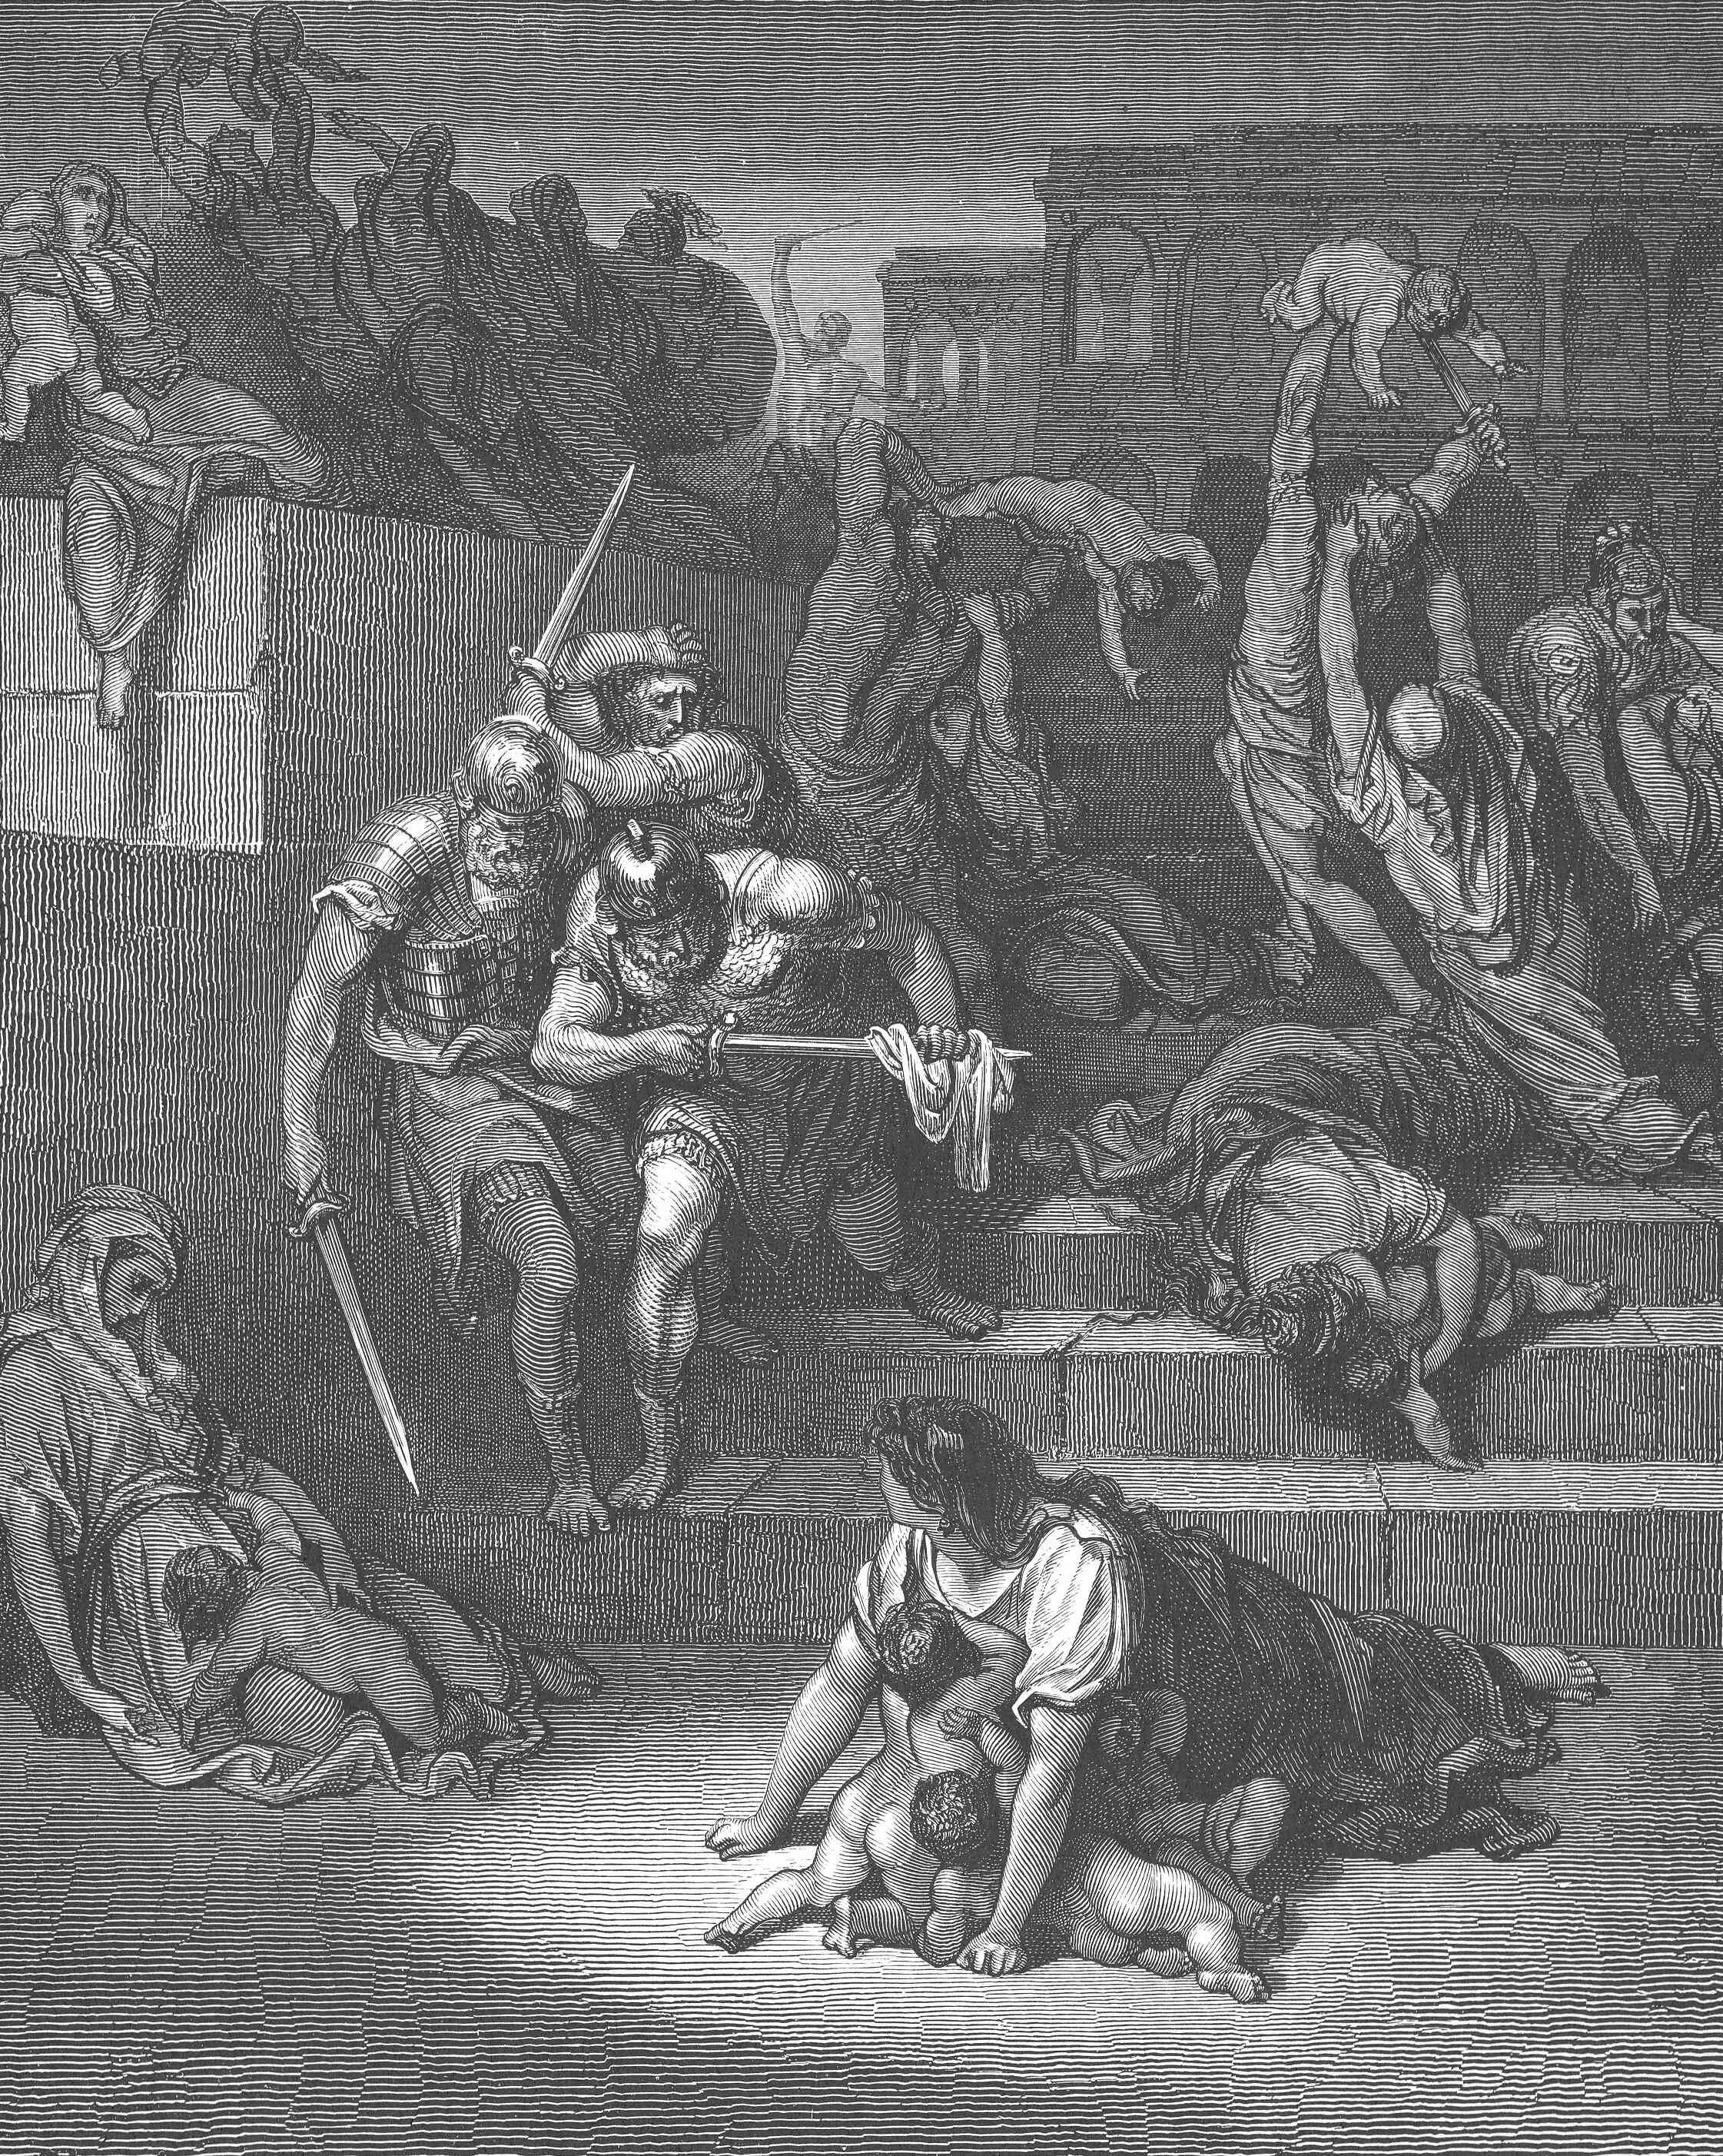
\includegraphics[width=.5\linewidth]{pics/E2C} \\[-.25em]
%		\pgfornament[width=.5\linewidth]{86}\\[.5em]
		\textsc{ the massacre of the innocents} \\[.5em]
		\begin{minipage}{.5\linewidth}\centering\small\itshape
			Then Herod (\ldots) was exceding worth (\ldots) and slew all the children that were in Bethlehem, and in all the coasts thereof, from two years old and under.\\ \normalfont
			(Matthew 2:16)
		\end{minipage}\vspace*{.25em}
			
\end{center}
%\vfill
%\begin{center}

%\end{center}

%\thispagestyle{plain}
\begin{multicols}{2}
\section{dedication}
\begin{flushright}
	\itshape To C. F G. Masterman, M. P.
\end{flushright}
My Dear Charles,\\ 
I originally called this book ``What is Wrong", and it would have
satisfied your sardonic temper to note the number of social
misunderstandings that arose from the use of the title. Many a mild lady
visitor opened her eyes when I remarked casually, ``I have been doing
`What is Wrong' all this morning". And one minister of religion moved
quite sharply in his chair when I told him (as he understood it) that I had to
run upstairs and do what was wrong, but should be down again in a minute.
Exactly of what occult vice they silently accused me I cannot conjecture,
but I know of what I accuse myself; and that is, of having written a very
shapeless and inadequate book, and one quite unworthy to be dedicated to
you. As far as literature goes, this book is what is wrong and no mistake.

It may seem a refinement of insolence to present so wild a
composition to one who has recorded two or three of the really impressive
visions of the moving millions of England. You are the only man alive
who can make the map of England crawl with life; a most creepy and
enviable accomplishment. Why then should I trouble you with a book
which, even if it achieves its object (which is monstrously unlikely) can
only be a thundering gallop of theory?

Well, I do it partly because I think you politicians are none the worse
for a few inconvenient ideals; but more because you will recognise the
many arguments we have had, those arguments which the most wonderful
ladies in the world can never endure for very long. And, perhaps, you will
agree with me that the thread of comradeship and conversation must be
protected because it is so frivolous. It must be held sacred, it must not be
snapped, because it is not worth tying together again. It is exactly because
argument is idle that men (I mean males) must take it seriously; for when
(we feel), until the crack of doom, shall we have so delightful a difference
again? But most of all I offer it to you because there exists not only
comradeship, but a very different thing, called friendship; an agreement
under all the arguments and a thread which, please God, will never break. Yours always,
\begin{flushright}
	G. K. Chesterton.
\end{flushright}
\end{multicols}
\end{titlepage}


%\vfill
\chapter{\adforn{69} The homelesness \textit{of} man \adforn{41}}
\section{the medical mistake}
     \dcap{A}{book of modern}social inquiry has a shape that is somewhat sharply
defined. It begins as a rule with an analysis, with statistics, tables of
population, decrease of crime among Congregationalists, growth of
hysteria among policemen, and similar ascertained facts; it ends with a
chapter that is generally called ``The Remedy". It is almost wholly due to
this careful, solid, and scientific method that ``The Remedy" is never found.
For this scheme of medical question and answer is a blunder; the first
great blunder of sociology. It is always called stating the disease before we
find the cure. But it is the whole definition and dignity of man that in
social matters we must actually find the cure before we find the disease.

The fallacy is one of the fifty fallacies that come from the modern
madness for biological or bodily metaphors. It is convenient to speak of
the Social Organism, just as it is convenient to speak of the British Lion.
But Britain is no more an organism than Britain is a lion. The moment we
begin to give a nation the unity and simplicity of an animal, we begin to
think wildly. 

Because every man is a biped, fifty men are not a centipede.
This has produced, for instance, the gaping absurdity of perpetually
talking about ``young nations" and ``dying nations", as if a nation had a
fixed and physical span of life. Thus people will say that Spain has entered
a final senility; they might as well say that Spain is losing all her teeth. Or
people will say that Canada should soon produce a literature; which is like
saying that Canada must soon grow a new moustache. Nations consist of
people; the first generation may be decrepit, or the ten thousandth may be
vigorous.

 Similar applications of the fallacy are made by those who see in
the increasing size of national possessions, a simple increase in wisdom
and stature, and in favor with God and man. These people, indeed, even
fall short in subtlety of the parallel of a human body. They do not even ask
whether an empire is growing taller in its youth, or only growing fatter in
its old age. But of all the instances of error arising from this physical fancy,
the worst is that we have before us: the habit of exhaustively describing a
social sickness, and then propounding a social drug.

Now we do talk first about the disease in cases of bodily breakdown;
and that for an excellent reason. Because, though there may be doubt
about the way in which the body broke down, there is no doubt at all about
the shape in which it should be built up again. No doctor proposes to
produce a new kind of man, with a new arrangement of eyes or limbs. The
hospital, by necessity, may send a man home with one leg less: but it will
not (in a creative rapture) send him home with one leg extra. Medical
science is content with the normal human body, and only seeks to restore
it.

But social science is by no means always content with the normal
human soul; it has all sorts of fancy souls for sale. Man as a social idealist
will say ``I am tired of being a Puritan; I want to be a Pagan", or ``Beyond
this dark probation of Individualism I see the shining paradise of
Collectivism".

 Now in bodily ills there is none of this difference about the
ultimate ideal. The patient may or may not want quinine; but he certainly
wants health No one says ``I am tired of this headache; I want some
toothache", or ``The only thing for this Russian influenza is a few German
measles", or ``Through this dark probation of catarrh I see the shining
paradise of rheumatism". 

But exactly the whole difficulty in our public
problems is that some men are aiming at cures which other men would
regard as worse maladies; are offering ultimate conditions as states of
health which others would uncompromisingly call states of disease. Mr.
Belloc once said that he would no more part with the idea of property than
with his teeth; yet to Mr. Bernard Shaw property is not a tooth, but a
toothache. Lord Milner has sincerely attempted to introduce German
efficiency; and many of us would as soon welcome German measles. Dr.
Saleeby would honestly like to have Eugenics; but I would rather have
rheumatics.

This is the arresting and dominant fact about modern social discussion;
that the quarrel is not merely about the difficulties, but about the aim. 

We agree about the evil; it is about the good that we should tear each other's
eyes cut. We all admit that a lazy aristocracy is a bad thing. We should not
by any means all admit that an active aristocracy would be a good thing.
We all feel angry with an irreligious priesthood; but some of us would go
mad with disgust at a really religious one. Everyone is indignant if our
army is weak, including the people who would be even more indignant if
it were strong. 

The social case is exactly the opposite of the medical case.
We do not disagree, like doctors, about the precise nature of the illness,
while agreeing about the nature of health. On the contrary, we all agree
that England is unhealthy, but half of us would not look at her in what the
other half would call blooming health . Public abuses are so prominent and
pestilent that they sweep all generous people into a sort of fictitious
unanimity. We forget that, while we agree about the abuses of things, we
should differ very much about the uses of them. Mr. Cadbury and I would
agree about the bad public house. It would be precisely in front of the
good public-house that our painful personal fracas would occur.

I maintain, therefore, that the common sociological method is quite
useless: that of first dissecting abject poverty or cataloguing prostitution.
We all dislike abject poverty; but it might be another business if we began
to discuss independent and dignified poverty. We all disapprove of
prostitution; but we do not all approve of purity. The only way to discuss
the social evil is to get at once to the social ideal. We can all see the
national madness; but what is national sanity? I have called this book
``What Is Wrong with the World?" and the upshot of the title can be easily
and clearly stated. What is wrong is that we do not ask what is right.

\section{wanted, an unpractical man}

There is a popular philosophical joke intended to typify the endless
and useless arguments of philosophers; I mean the joke about which came
first, the chicken or the egg? I am not sure that properly understood, it is
so futile an inquiry after all. 

I am not concerned here to enter on those
deep metaphysical and theological differences of which the chicken and
egg debate is a frivolous, but a very felicitous, type. The evolutionary
materialists are appropriately enough represented in the vision of all things
coming from an egg, a dim and monstrous oval germ that had laid itself by
accident. That other supernatural school of thought (to which I personally
adhere) would be not unworthily typified in the fancy that this round
world of ours is but an egg brooded upon by a sacred unbegotten bird; the
mystic dove of the prophets. But it is to much humbler functions that I
here call the awful power of such a distinction. Whether or no the living
bird is at the beginning of our mental chain, it is absolutely necessary that
it should be at the end of our mental chain. The bird is the thing to be
aimed at--not with a gun, but a life-bestowing wand. 

What is essential to
our right thinking is this: that the egg and the bird must not be thought of
as equal cosmic occurrences recurring alternatively forever. They must not
become a mere egg and bird pattern, like the egg and dart pattern. One is a
means and the other an end; they are in different mental worlds. Leaving
the complications of the human breakfast-table out of account, in an
elemental sense, the egg only exists to produce the chicken. But the
chicken does not exist only in order to produce another egg. He may also
exist to amuse himself, to praise God, and even to suggest ideas to a
French dramatist. Being a conscious life, he is, or may be, valuable in
himself. Now our modern politics are full of a noisy forgetfulness;
forgetfulness that the production of this happy and conscious life is after
all the aim of all complexities and compromises. 

We talk of nothing but
useful men and working institutions; that is, we only think of the chickens
as things that will lay more eggs. Instead of seeking to breed our ideal bird,
the eagle of Zeus or the Swan of Avon, or whatever we happen to want,
we talk entirely in terms of the process and the embryo. The process itself,
divorced from its divine object, becomes doubtful and even morbid;
poison enters the embryo of everything; and our politics are rotten eggs.

     Idealism is only considering everything in its practical essence.
Idealism only means that we should consider a poker in reference to
poking before we discuss its suitability for wife-beating; that we should
ask if an egg is good enough for practical poultry-rearing before we decide
that the egg is bad enough for practical politics. But I know that this
primary pursuit of the theory (which is but pursuit of the aim) exposes one
to the cheap charge of fiddling while Rome is burning. A school, of which
Lord Rosebery is representative, has endeavored to substitute for the
moral or social ideals which have hitherto been the motive of politics a
general coherency or completeness in the social system which has gained
the nick-name of ``efficiency". I am not very certain of the secret doctrine
of this sect in the matter. 

But, as far as I can make out, ``efficiency" means
that we ought to discover everything about a machine except what it is for.
There has arisen in our time a most singular fancy: the fancy that when
things go very wrong we need a practical man. It would be far truer to say,
that when things go very wrong we need an unpractical man. Certainly, at
least, we need a theorist. A practical man means a man accustomed to
mere daily practice, to the way things commonly work. When things will
not work, you must have the thinker, the man who has some doctrine
about why they work at all. It is wrong to fiddle while Rome is burning;
but it is quite right to study the theory of hydraulics while Rome is
burning.

It is then necessary to drop one's daily agnosticism and attempt rerum
cognoscere causas. If your aeroplane has a slight indisposition, a handy
man may mend it. But, if it is seriously ill, it is all the more likely that
some absent-minded old professor with wild white hair will have to be
dragged out of a college or laboratory to analyze the evil. The more
complicated the smash, the whiter-haired and more absent-minded will be
the theorist who is needed to deal with it; and in some extreme cases, no
one but the man (probably insane) who invented your flying-ship could
possibly say what was the matter with it.

``Efficiency", of course, is futile for the same reason that strong men,
will-power and the superman are futile. That is, it is futile because it only
deals with actions after they have been performed. It has no philosophy for
incidents before they happen; therefore it has no power of choice. An act
can only be successful or unsuccessful when it is over; if it is to begin, it
must be, in the abstract, right or wrong. 

There is no such thing as backing
a winner; for he cannot be a winner when he is backed. There is no such
thing as fighting on the winning side; one fights to find out which is the
winning side. If any operation has occurred, that operation was efficient. If
a man is murdered, the murder was efficient. A tropical sun is as efficient
in making people lazy as a Lancashire foreman bully in making them
energetic. Maeterlinck is as efficient in filling a man with strange spiritual
tremors as Messrs. Crosse and Blackwell are in filling a man with jam.
But it all depends on what you want to be filled with. 

Lord Rosebery,
being a modern skeptic, probably prefers the spiritual tremors. I, being an
orthodox Christian, prefer the jam. But both are efficient when they have
been effected; and inefficient until they are effected. A man who thinks
much about success must be the drowsiest sentimentalist; for he must be
always looking back. If he only likes victory he must always come late for
the battle. For the man of action there is nothing but idealism.

This definite ideal is a far more urgent and practical matter in our
existing English trouble than any immediate plans or proposals. For the
present chaos is due to a sort of general oblivion of all that men were
originally aiming at. No man demands what he desires; each man demands
what he fancies he can get. Soon people forget what the man really wanted
first; and after a successful and vigorous political life, he forgets it himself.
The whole is an extravagant riot of second bests, a pandemonium of pis-
aller. 

Now this sort of pliability does not merely prevent any heroic
consistency, it also prevents any really practical compromise. One can
only find the middle distance between two points if the two points will
stand still. We may make an arrangement between two litigants who
cannot both get what they want; but not if they will not even tell us what
they want. The keeper of a restaurant would much prefer that each
customer should give his order smartly, though it were for stewed ibis or
boiled elephant, rather than that each customer should sit holding his head
in his hands, plunged in arithmetical calculations about how much food
there can be on the premises. 

Most of us have suffered from a certain sort
of ladies who, by their perverse unselfishness, give more trouble than the
selfish; who almost clamor for the unpopular dish and scramble for the
worst seat. Most of us have known parties or expeditions full of this
seething fuss of self-effacement. From much meaner motives than those of
such admirable women, our practical politicians keep things in the same
confusion through the same doubt about their real demands. There is
nothing that so much prevents a settlement as a tangle of small surrenders.
We are bewildered on every side by politicians who are in favor of secular
education, but think it hopeless to work for it; who desire total prohibition,
but are certain they should not demand it; who regret compulsory
education, but resignedly continue it; or who want peasant proprietorship
and therefore vote for something else. 

It is this dazed and floundering
opportunism that gets in the way of everything. If our statesmen were
visionaries something practical might be done. If we ask for something in
the abstract we might get something in the concrete. As it is, it is not only
impossible to get what one wants, but it is impossible to get any part of it,
because nobody can mark it out plainly like a map. That clear and even
hard quality that there was in the old bargaining has wholly vanished. We
forget that the word ``compromise" contains, among other things, the rigid
and ringing word ``promise". Moderation is not vague; it is as definite as
perfection. The middle point is as fixed as the extreme point.

If I am made to walk the plank by a pirate, it is vain for me to offer, as
a common-sense compromise, to walk along the plank for a reasonable
distance. It is exactly about the reasonable distance that the pirate and I
differ. There is an exquisite mathematical split second at which the plank
tips up. My common-sense ends just before that instant; the pirate's
common-sense begins just beyond it. But the point itself is as hard as any
geometrical diagram; as abstract as any theological dogma.

\section{the new hypocrite}
But this new cloudy political cowardice has rendered useless the old
English compromise. People have begun to be terrified of an improvement
merely because it is complete. They call it utopian and revolutionary that
anyone should really have his own way, or anything be really done, and
done with. Compromise used to mean that half a loaf was better than no
bread. Among modern statesmen it really seems to mean that half a loaf is
better than a whole loaf.

    As an instance to sharpen the argument, I take the one case of our
everlasting education bills. We have actually contrived to invent a new
kind of hypocrite. The old hypocrite, Tartuffe or Pecksniff, was a man
whose aims were really worldly and practical, while he pretended that they
were religious. The new hypocrite is one whose aims are really religious,
while he pretends that they are worldly and practical. 

The Rev. Brown, the
Wesleyan minister, sturdily declares that he cares nothing for creeds, but
only for education; meanwhile, in truth, the wildest Wesleyanism is
tearing his soul. The Rev. Smith, of the Church of England, explains
gracefully, with the Oxford manner, that the only question for him is the
prosperity and efficiency of the schools; while in truth all the evil passions
of a curate are roaring within him. It is a fight of creeds masquerading as
policies. I think these reverend gentlemen do themselves wrong; I think
they are more pious than they will admit. Theology is not (as some
suppose) expunged as an error. It is merely concealed, like a sin. Dr.
Clifford really wants a theological atmosphere as much as Lord Halifax;
only it is a different one. If Dr. Clifford would ask plainly for Puritanism
and Lord Halifax ask plainly for Catholicism, something might be done
for them. We are all, one hopes, imaginative enough to recognize the
dignity and distinctness of another religion, like Islam or the cult of Apollo.

I am quite ready to respect another man's faith; but it is too much to ask
that I should respect his doubt, his worldly hesitations and fictions, his
political bargain and make-believe. Most Nonconformists with an instinct
for English history could see something poetic and national about the
Archbishop of Canterbury as an Archbishop of Canterbury. It is when he
does the rational British statesman that they very justifiably get annoyed.
Most Anglicans with an eye for pluck and simplicity could admire Dr.
Clifford as a Baptist minister. It is when he says that he is simply a citizen
that nobody can possibly believe him.

But indeed the case is yet more curious than this. The one argument
that used to be urged for our creedless vagueness was that at least it saved
us from fanaticism. But it does not even do that. On the contrary, it creates
and renews fanaticism with a force quite peculiar to itself. This is at once
so strange and so true that I will ask the reader's attention to it with a little more precision.

Some people do not like the word ``dogma". Fortunately they are free,
and there is an alternative for them. There are two things, and two things
only, for the human mind, a dogma and a prejudice. The Middle Ages
were a rational epoch, an age of doctrine. Our age is, at its best, a poetical
epoch, an age of prejudice. A doctrine is a definite point; a prejudice is a
direction. That an ox may be eaten, while a man should not be eaten, is a
doctrine. That as little as possible of anything should be eaten is a
prejudice; which is also sometimes called an ideal. Now a direction is
always far more fantastic than a plan. 

I would rather have the most archaic
map of the road to Brighton than a general recommendation to turn to the
left. Straight lines that are not parallel must meet at last; but curves may
recoil forever. A pair of lovers might walk along the frontier of France and
Germany, one on the one side and one on the other, so long as they were
not vaguely told to keep away from each other. And this is a strictly true
parable of the effect of our modern vagueness in losing and separating
men as in a mist.

It is not merely true that a creed unites men. Nay, a difference of creed
unites men--so long as it is a clear difference. A boundary unites. Many a
magnanimous Moslem and chivalrous Crusader must have been nearer to
each other, because they were both dogmatists, than any two homeless
agnostics in a pew of Mr. Campbell's chapel. ``I say God is One", and ``I
say God is One but also Three", that is the beginning of a good
quarrelsome, manly friendship. 

But our age would turn these creeds into
tendencies. It would tell the Trinitarian to follow multiplicity as such
(because it was his ``temperament"), and he would turn up later with three
hundred and thirty-three persons in the Trinity. Meanwhile, it would turn
the Moslem into a Monist: a frightful intellectual fall. It would force that
previously healthy person not only to admit that there was one God, but to
admit that there was nobody else. When each had, for a long enough
period, followed the gleam of his own nose (like the Dong) they would
appear again; the Christian a Polytheist, and the Moslem a Panegoist, both
quite mad, and far more unfit to understand each other than before.

It is exactly the same with politics. Our political vagueness divides
men, it does not fuse them. Men will walk along the edge of a chasm in
clear weather, but they will edge miles away from it in a fog. So a Tory
can walk up to the very edge of Socialism, if he knows what is Socialism.
But if he is told that Socialism is a spirit, a sublime atmosphere, a noble,
indefinable tendency, why, then he keeps out of its way; and quite right
too. One can meet an assertion with argument; but healthy bigotry is the
only way in which one can meet a tendency. I am told that the Japanese
method of wrestling consists not of suddenly pressing, but of suddenly
giving way. This is one of my many reasons for disliking the Japanese
civilization. To use surrender as a weapon is the very worst spirit of the
East. 

But certainly there is no force so hard to fight as the force which it is
easy to conquer; the force that always yields and then returns. Such is the
force of a great impersonal prejudice, such as possesses the modern world
on so many points. Against this there is no weapon at all except a rigid and
steely sanity, a resolution not to listen to fads, and not to be infected by
diseases.

In short, the rational human faith must armor itself with prejudice in an
age of prejudices, just as it armoured itself with logic in an age of logic.
But the difference between the two mental methods is marked and
unmistakable. The essential of the difference is this: that prejudices are
divergent, whereas creeds are always in collision. Believers bump into
each other; whereas bigots keep out of each other's way. A creed is a
collective thing, and even its sins are sociable. A prejudice is a private
thing, and even its tolerance is misanthropic. 

So it is with our existing
divisions. They keep out of each other's way; the Tory paper and the
Radical paper do not answer each other; they ignore each other. Genuine
controversy, fair cut and thrust before a common audience, has become in
our special epoch very rare. For the sincere controversialist is above all
things a good listener. The really burning enthusiast never interrupts; he
listens to the enemy's arguments as eagerly as a spy would listen to the
enemy's arrangements. But if you attempt an actual argument with a
modern paper of opposite politics, you will find that no medium is
admitted between violence and evasion. You will have no answer except
slanging or silence. A modern editor must not have that eager ear that goes
with the honest tongue. He may be deaf and silent; and that is called
dignity. Or he may be deaf and noisy; and that is called slashing
journalism. In neither case is there any controversy; for the whole object
of modern party combatants is to charge out of earshot.

The only logical cure for all this is the assertion of a human ideal. In
dealing with this, I will try to be as little transcendental as is consistent
with reason; it is enough to say that unless we have some doctrine of a
divine man, all abuses may be excused, since evolution may turn them into
uses. It will be easy for the scientific plutocrat to maintain that humanity
will adapt itself to any conditions which we now consider evil. The old
tyrants invoked the past; the new tyrants will invoke the future evolution
has produced the snail and the owl; evolution can produce a workman who
wants no more space than a snail, and no more light than an owl. 

The
employer need not mind sending a Kaffir to work underground; he will
soon become an underground animal, like a mole. He need not mind
sending a diver to hold his breath in the deep seas; he will soon be a deep-
sea animal. Men need not trouble to alter conditions, conditions will so
soon alter men. The head can be beaten small enough to fit the hat. Do not
knock the fetters off the slave; knock the slave until he forgets the fetters.
To all this plausible modem argument for oppression, the only adequate
answer is, that there is a permanent human ideal that must not be either
confused or destroyed. The most important man on earth is the perfect
man who is not there. The Christian religion has specially uttered the
ultimate sanity of Man, says Scripture, who shall judge the incarnate and
human truth. Our lives and laws are not judged by divine superiority, but
simply by human perfection. It is man, says Aristotle, who is the measure.
It is the Son of Man, says Scripture, who shall judge the quick and the
dead.

Doctrine, therefore, does not cause dissensions; rather a doctrine alone
can cure our dissensions. It is necessary to ask, however, roughly, what
abstract and ideal shape in state or family would fulfil the human hunger;
and this apart from whether we can completely obtain it or not. But when
we come to ask what is the need of normal men, what is the desire of all
nations, what is the ideal house, or road, or rule, or republic, or king, or
priesthood, then we are confronted with a strange and irritating difficulty
peculiar to the present time; and we must call a temporary halt and
examine that obstacle.

\section{the fear of the past}

The last few decades have been marked by a special cultivation of the
romance of the future. We seem to have made up our minds to
misunderstand what has happened; and we turn, with a sort of relief, to
stating what will happen--which is (apparently) much easier.

 The modern
man no longer presents the memoirs of his great grandfather; but is
engaged in writing a detailed and authoritative biography of his great-
grandson. Instead of trembling before the specters of the dead, we shudder
abjectly under the shadow of the babe unborn. This spirit is apparent
everywhere, even to the creation of a form of futurist romance. Sir Walter
Scott stands at the dawn of the nineteenth century for the novel of the past;
Mr. H. G. Wells stands at the dawn of the twentieth century for the novel
of the future. The old story, we know, was supposed to begin: 
\begin{quotation}\noindent
	``Late on a
	winter's evening two horsemen might have been seen--".
\end{quotation}
The new story has to begin: 
\begin{quotation}\noindent
	``Late on a winter's evening two aviators will be seen--".
\end{quotation}
The
movement is not without its elements of charm; there is something spirited,
if eccentric, in the sight of so many people fighting over again the fights
that have not yet happened; of people still glowing with the memory of
tomorrow morning. A man in advance of the age is a familiar phrase
enough. An age in advance of the age is really rather odd.

But when full allowance has been made for this harmless element of
poetry and pretty human perversity in the thing, I shall not hesitate to
maintain here that this cult of the future is not only a weakness but a
cowardice of the age. It is the peculiar evil of this epoch that even its
pugnacity is fundamentally frightened; and the Jingo is contemptible not
because he is impudent, but because he is timid.

 The reason why modern
armaments do not inflame the imagination like the arms and
emblazonments of the Crusades is a reason quite apart from optical
ugliness or beauty. Some battleships are as beautiful as the sea; and many
Norman nosepieces were as ugly as Norman noses. The atmospheric
ugliness that surrounds our scientific war is an emanation from that evil
panic which is at the heart of it.

 The charge of the Crusades was a charge;
it was charging towards God, the wild consolation of the braver. The
charge of the modern armaments is not a charge at all. It is a rout, a retreat,
a flight from the devil, who will catch the hindmost. It is impossible to
imagine a mediaeval knight talking of longer and longer French lances,
with precisely the quivering employed about larger and larger German
ships The man who called the Blue Water School the ``Blue Funk School"
uttered a psychological truth which that school itself would scarcely
essentially deny. Even the two-power standard, if it be a necessity, is in a
sense a degrading necessity. Nothing has more alienated many
magnanimous minds from Imperial enterprises than the fact that they are
always exhibited as stealthy or sudden defenses against a world of cold
rapacity and fear. 

The Boer War, for instance, was colored not so much by
the creed that we were doing something right, as by the creed that Boers
and Germans were probably doing something wrong; driving us (as it was
said) to the sea. Mr. Chamberlain, I think, said that the war was a feather
in his cap and so it was: a white feather.

Now this same primary panic that I feel in our rush towards patriotic
armaments I feel also in our rush towards future visions of society. The
modern mind is forced towards the future by a certain sense of fatigue, not
unmixed with terror, with which it regards the past. It is propelled towards
the coming time; it is, in the exact words of the popular phrase, knocked
into the middle of next week. 

And the goad which drives it on thus eagerly
is not an affectation for futurity Futurity does not exist, because it is still
future. Rather it is a fear of the past; a fear not merely of the evil in the
past, but of the good in the past also. The brain breaks down under the
unbearable virtue of mankind. There have been so many flaming faiths
that we cannot hold; so many harsh heroisms that we cannot imitate; so
many great efforts of monumental building or of military glory which
seem to us at once sublime and pathetic. 

The future is a refuge from the
fierce competition of our forefathers. The older generation, not the
younger, is knocking at our door. It is agreeable to escape, as Henley said,
into the Street of By-and-Bye, where stands the Hostelry of Never. It is
pleasant to play with children, especially unborn children. The future is a
blank wall on which every man can write his own name as large as he
likes; the past I find already covered with illegible scribbles, such as Plato,
Isaiah, Shakespeare, Michael Angelo, Napoleon.

 I can make the future as
narrow as myself; the past is obliged to be as broad and turbulent as
humanity. And the upshot of this modern attitude is really this: that men
invent new ideals because they dare not attempt old ideals. They look
forward with enthusiasm, because they are afraid to look back.

Now in history there is no Revolution that is not a Restoration. Among
the many things that Leave me doubtful about the modern habit of fixing
eyes on the future, none is stronger than this: that all the men in history
who have really done anything with the future have had their eyes fixed
upon the past. 

I need not mention the Renaissance, the very word proves
my case. The originality of Michael Angelo and Shakespeare began with
the digging up of old vases and manuscripts. The mildness of poets
absolutely arose out of the mildness of antiquaries. So the great mediaeval
revival was a memory of the Roman Empire. So the Reformation looked
back to the Bible and Bible times. 

So the modern Catholic movement has
looked back to patristic times. But that modern movement which many
would count the most anarchic of all is in this sense the most conservative
of all. Never was the past more venerated by men than it was by the
French Revolutionists. They invoked the little republics of antiquity with
the complete confidence of one who invokes the gods. The Sans-culottes
believed (as their name might imply) in a return to simplicity. They
believed most piously in a remote past; some might call it a mythical past.
For some strange reason man must always thus plant his fruit trees in a
graveyard. 

Man can only find life among the dead. Man is a misshapen
monster, with his feet set forward and his face turned back. He can make
the future luxuriant and gigantic, so long as he is thinking about the past.
When he tries to think about the future itself, his mind diminishes to a pin
point with imbecility, which some call Nirvana. To-morrow is the Gorgon;
a man must only see it mirrored in the shining shield of yesterday. If he
sees it directly he is turned to stone. This has been the fate of all those who
have really seen fate and futurity as clear and inevitable. The Calvinists,
with their perfect creed of predestination, were turned to stone. 

The
modern sociological scientists (with their excruciating Eugenics) are
turned to stone. The only difference is that the Puritans make dignified,
and the Eugenists somewhat amusing, statues.

But there is one feature in the past which more than all the rest defies
and depresses the moderns and drives them towards this featureless future.
I mean the presence in the past of huge ideals, unfulfilled and sometimes
abandoned. The sight of these splendid failures is melancholy to a restless
and rather morbid generation; and they maintain a strange silence about
them--sometimes amounting to an unscrupulous silence. They keep them
entirely out of their newspapers and almost entirely out of their history
books. For example, they will often tell you (in their praises of the coming
age) that we are moving on towards a United States of Europe. But they
carefully omit to tell you that we are moving away from a United States of
Europe, that such a thing existed literally in Roman and essentially in
mediaeval times. They never admit that the international hatreds (which
they call barbaric) are really very recent, the mere breakdown of the ideal
of the Holy Roman Empire. Or again, they will tell you that there is going
to be a social revolution, a great rising of the poor against the rich; but
they never rub it in that France made that magnificent attempt, unaided,
and that we and all the world allowed it to be trampled out and forgotten. I
say decisively that nothing is so marked in modern writing as the
prediction of such ideals in the future combined with the ignoring of them
in the past. Anyone can test this for himself. Read any thirty or forty pages
of pamphlets advocating peace in Europe and see how many of them
praise the old Popes or Emperors for keeping the peace in Europe. Read
any armful of essays and poems in praise of social democracy, and see
how many of them praise the old Jacobins who created democracy and
died for it. These colossal ruins are to the modern only enormous eyesores.
He looks back along the valley of the past and sees a perspective of
splendid but unfinished cities. They are unfinished, not always through
enmity or accident, but often through fickleness, mental fatigue, and the
lust for alien philosophies. We have not only left undone those things that
we ought to have done, but we have even left undone those things that we
wanted to do.

It is very currently suggested that the modern man is the heir of all the
ages, that he has got the good out of these successive human experiments.
I know not what to say in answer to this, except to ask the reader to look at
the modern man, as I have just looked at the modern man-- in the looking-
glass. Is it really true that you and I are two starry towers built up of all the
most towering visions of the past? Have we really fulfilled all the great
historic ideals one after the other, from our naked ancestor who was brave
enough to till a mammoth with a stone knife, through the Greek citizen
and the Christian saint to our own grandfather or great-grandfather, who
may have been sabred by the Manchester Yeomanry or shot in the '48? Are
we still strong enough to spear mammoths, but now tender enough to
spare them? Does the cosmos contain any mammoth that we have either
speared or spared? When we decline (in a marked manner) to fly the red
flag and fire across a barricade like our grandfathers, are we really
declining in deference to sociologists--or to soldiers? Have we indeed
outstripped the warrior and passed the ascetical saint? I fear we only
outstrip the warrior in the sense that we should probably run away from
him. And if we have passed the saint, I fear we have passed him without
bowing.

This is, first and foremost, what I mean by the narrowness of the new
ideas, the limiting effect of the future. Our modern prophetic idealism is
narrow because it has undergone a persistent process of elimination. We
must ask for new things because we are not allowed to ask for old things.
The whole position is based on this idea that we have got all the good that
can be got out of the ideas of the past. But we have not got all the good out
of them, perhaps at this moment not any of the good out of them. And the
need here is a need of complete freedom for restoration as well as
revolution.

We often read nowadays of the valor or audacity with which some
rebel attacks a hoary tyranny or an antiquated superstition. There is not
really any courage at all in attacking hoary or antiquated things, any more
than in offering to fight one's grandmother. The really courageous man is
he who defies tyrannies young as the morning and superstitions fresh as
the first flowers. The only true free-thinker is he whose intellect is as
much free from the future as from the past. He cares as little for what will
be as for what has been; he cares only for what ought to be. And for my
present purpose I specially insist on this abstract independence. If I am to
discuss what is wrong, one of the first things that are wrong is this: the
deep and silent modern assumption that past things have become
impossible. There is one metaphor of which the moderns are very fond;
they are always saying, ``You can't put the clock back". The simple and
obvious answer is ``You can". A clock, being a piece of human
construction, can be restored by the human finger to any figure or hour. In
the same way society, being a piece of human construction, can be
reconstructed upon any plan that has ever existed.

There is another proverb,
\begin{quotation}\noindent
	``As you have made your bed, so you must
	lie on it";
\end{quotation}
 which again is simply a lie. If I have made my bed
uncomfortable, please God I will make it again. We could restore the
Heptarchy or the stage coaches if we chose. It might take some time to do,
and it might be very inadvisable to do it; but certainly it is not impossible
as bringing back last Friday is impossible. This is, as I say, the first
freedom that I claim: the freedom to restore. I claim a right to propose as a
solution the old patriarchal system of a Highland clan, if that should seem
to eliminate the largest number of evils. It certainly would eliminate some
evils; for instance, the unnatural sense of obeying cold and harsh strangers,
mere bureaucrats and policemen. I claim the right to propose the complete
independence of the small Greek or Italian towns, a sovereign city of
Brixton or Brompton, if that seems the best way out of our troubles. It
would be a way out of some of our troubles; we could not have in a small
state, for instance, those enormous illusions about men or measures which
are nourished by the great national or international newspapers. You could
not persuade a city state that Mr. Beit was an Englishman, or Mr. Dillon a
desperado, any more than you could persuade a Hampshire Village that the
village drunkard was a teetotaller or the village idiot a statesman.
Nevertheless, I do not as a fact propose that the Browns and the Smiths
should be collected under separate tartans. Nor do I even propose that
Clapham should declare its independence. I merely declare my
independence. I merely claim my choice of all the tools in the universe;
and I shall not admit that any of them are blunted merely because they
have been used.

\section{the unfinished temple}

    The task of modern idealists indeed is made much too easy for them
by the fact that they are always taught that if a thing has been defeated it
has been disproved. Logically, the case is quite clearly the other way. The
lost causes are exactly those which might have saved the world. If a man
says that the Young Pretender would have made England happy, it is hard
to answer him. If anyone says that the Georges made England happy, I
hope we all know what to answer. That which was prevented is always
impregnable; and the only perfect King of England was he who was
smothered. Exactly be cause Jacobitism failed we cannot call it a failure.
Precisely because the Commune collapsed as a rebellion we cannot say
that it collapsed as a system. But such outbursts were brief or incidental.
Few people realize how many of the largest efforts, the facts that will fill
history, were frustrated in their full design and come down to us as
gigantic cripples. I have only space to allude to the two largest facts of
modern history: the Catholic Church and that modern growth rooted in the
French Revolution.

When four knights scattered the blood and brains of St. Thomas of
Canterbury, it was not only a sign of anger but of a sort of black
admiration. They wished for his blood, but they wished even more for his
brains. Such a blow will remain forever unintelligible unless we realise
what the brains of St. Thomas were thinking about just before they were
distributed over the floor. They were thinking about the great mediaeval
conception that the church is the judge of the world. Becket objected to a
priest being tried even by the Lord Chief Justice. And his reason was
simple: because the Lord Chief Justice was being tried by the priest. The
judiciary was itself sub judice. The kings were themselves in the dock.
The idea was to create an invisible kingdom, without armies or prisons,
but with complete freedom to condemn publicly all the kingdoms of the
earth. Whether such a supreme church would have cured society we
cannot affirm definitely; because the church never was a supreme church.
We only know that in England at any rate the princes conquered the saints.
What the world wanted we see before us; and some of us call it a failure.
But we cannot call what the church wanted a failure, simply because the
church failed. Tracy struck a little too soon. England had not yet made the
great Protestant discovery that the king can do no wrong. The king was
whipped in the cathedral; a performance which I recommend to those who
regret the unpopularity of church-going. But the discovery was made; and
Henry \textsc{viii} scattered Becket's bones as easily as Tracy had scattered his
brains.

Of course, I mean that Catholicism was not tried; plenty of Catholics
were tried, and found guilty. My point is that the world did not tire of the
church's ideal, but of its reality. Monasteries were impugned not for the
chastity of monks, but for the unchastity of monks. Christianity was
unpopular not because of the humility, but of the arrogance of Christians.
Certainly, if the church failed it was largely through the churchmen. But at
the same time hostile elements had certainly begun to end it long before it
could have done its work. In the nature of things it needed a common
scheme of life and thought in Europe. Yet the mediaeval system began to
be broken to pieces intellectually, long before it showed the slightest hint
of falling to pieces morally. The huge early heresies, like the Albigenses,
had not the faintest excuse in moral superiority. And it is actually true that
the Reformation began to tear Europe apart before the Catholic Church
had had time to pull it together. The Prussians, for instance, were not
converted to Christianity at all until quite close to the Reformation. The
poor creatures hardly had time to become Catholics before they were told
to become Protestants. This explains a great deal of their subsequent
conduct. But I have only taken this as the first and most evident case of the
general truth: that the great ideals of the past failed not by being outlived
(which must mean over-lived), but by not being lived enough. Mankind
has not passed through the Middle Ages. Rather mankind has retreated
from the Middle Ages in reaction and rout. The Christian ideal has not
been tried and found wanting. It has been found difficult; and left untried.

It is, of course, the same in the case of the French Revolution. A great
part of our present perplexity arises from the fact that the French
Revolution has half succeeded and half failed. In one sense, Valmy was
the decisive battle of the West, and in another Trafalgar. We have, indeed,
destroyed the largest territorial tyrannies, and created a free peasantry in
almost all Christian countries except England; of which we shall say more
anon. But representative government, the one universal relic, is a very
poor fragment of the full republican idea. 

The theory of the French
Revolution presupposed two things in government, things which it
achieved at the time, but which it has certainly not bequeathed to its
imitators in England, Germany, and America. The first of these was the
idea of honorable poverty; that a statesman must be something of a stoic;
the second was the idea of extreme publicity. Many imaginative English
writers, including Carlyle, seem quite unable to imagine how it was that
men like Robespierre and Marat were ardently admired. The best answer
is that they were admired for being poor-- poor when they might have
been rich.

No one will pretend that this ideal exists at all in the haute politique of
this country. Our national claim to political incorruptibility is actually
based on exactly the opposite argument; it is based on the theory that
wealthy men in assured positions will have no temptation to financial
trickery. Whether the history of the English aristocracy, from the
spoliation of the monasteries to the annexation of the mines, entirely
supports this theory I am not now inquiring; but certainly it is our theory,
that wealth will be a protection against political corruption. The English
statesman is bribed not to be bribed. He is born with a silver spoon in his
mouth, so that he may never afterwards be found with the silver spoons in
his pocket. 

So strong is our faith in this protection by plutocracy, that we
are more and more trusting our empire in the hands of families which
inherit wealth without either blood or manners. Some of our political
houses are parvenue by pedigree; they hand on vulgarity like a coat of-
arms. In the case of many a modern statesman to say that he is born with a
silver spoon in his mouth, is at once inadequate and excessive. He is born
with a silver knife in his mouth. But all this only illustrates the English
theory that poverty is perilous for a politician.

It will be the same if we compare the conditions that have come about
with the Revolution legend touching publicity. The old democratic
doctrine was that the more light that was let in to all departments of State,
the easier it was for a righteous indignation to move promptly against
wrong. In other words, monarchs were to live in glass houses, that mobs
might throw stones. 

Again, no admirer of existing English politics (if there
is any admirer of existing English politics) will really pretend that this
ideal of publicity is exhausted, or even attempted. Obviously public life
grows more private every day. The French have, indeed, continued the
tradition of revealing secrets and making scandals; hence they are more
flagrant and palpable than we, not in sin but in the confession of sin. The
first trial of Dreyfus might have happened in England; it is exactly the
second trial that would have been legally impossible. But, indeed, if we
wish to realise how far we fall short of the original republican outline, the
sharpest way to test it is to note how far we fall short even of the
republican element in the older regime. Not only are we less democratic
than Danton and Condorcet, but we are in many ways less democratic than
Choiseul and Marie Antoinette. 

The richest nobles before the revolt were
needy middle-class people compared with our Rothschilds and Roseberys.
And in the matter of publicity the old French monarchy was infinitely
more democratic than any of the monarchies of today. Practically anybody
who chose could walk into the palace and see the king playing with his
children, or paring his nails. The people possessed the monarch,, as the
people possess Primrose Hill; that is, they cannot move it, but they can
sprawl all over it. The old French monarchy was founded on the excellent
principle that a cat may look at a king. But nowadays a cat may not look at
a king; unless it is a very tame cat. Even where the press is free for
criticism it is only used for adulation. The substantial difference comes to
something uncommonly like this: Eighteenth century tyranny meant that
you could say ``The K\underline{\hspace{.2cm}} of Br\underline{\hspace{.2cm}}rd is a profligate". Twentieth century
liberty really means that you are allowed to say ``The King of Brentford is
a model family man".

But we have delayed the main argument too long for the parenthetical
purpose of showing that the great democratic dream, like the great
mediaeval dream, has in a strict and practical sense been a dream
unfulfilled. Whatever is the matter with modern England it is not that we
have carried out too literally, or achieved with disappointing completeness,
either the Catholicism of Becket or the equality of Marat. Now I have
taken these two cases merely because they are typical of ten thousand
other cases; the world is full of these unfulfilled ideas, these uncompleted
temples. History does not consist of completed and crumbling ruins; rather
it consists of half-built villas abandoned by a bankrupt-builder. This world
is more like an unfinished suburb than a deserted cemetery.

\section{the enemies of property}

    But it is for this especial reason that such an explanation is necessary
on the very threshold of the definition of ideals. For owing to that historic
fallacy with which I have just dealt, numbers of readers will expect me,
when I propound an ideal, to propound a new ideal. Now I have no notion
at all of propounding a new ideal. There is no new ideal imaginable by the
madness of modern sophists, which will be anything like so startling as
fulfilling any one of the old ones. On the day that any copybook maxim is
carried out there will be something like an earthquake on the earth. There
is only one thing new that can be done under the sun; and that is to look at
the sun. If you attempt it on a blue day in June, you will know why men
do not look straight at their ideals. There is only one really startling thing
to be done with the ideal, and that is to do it. It is to face the flaming
logical fact, and its frightful consequences. Christ knew that it would be a
more stunning thunderbolt to fulfil the law than to destroy it. It is true of
both the cases I have quoted, and of every case. The pagans had always
adored purity: Athena, Artemis, Vesta. It was when the virgin martyrs
began defiantly to practice purity that they rent them with wild beasts, and
rolled them on red-hot coals. The world had always loved the notion of the
poor man uppermost; it can be proved by every legend from Cinderella to
Whittington, by every poem from the Magnificat to the Marseillaise. The
kings went mad against France not because she idealized this ideal, but
because she realized it. Joseph of Austria and Catherine of Russia quite
agreed that the people should rule; what horrified them was that the people
did. The French Revolution, therefore, is the type of all true revolutions,
because its ideal is as old as the Old Adam, but its fulfilment almost as
fresh, as miraculous, and as new as the New Jerusalem.

But in the modern world we are primarily confronted with the
extraordinary spectacle of people turning to new ideals because they have
not tried the old. Men have not got tired of Christianity; they have never
found enough Christianity to get tired of. Men have never wearied of
political justice; they have wearied of waiting for it.

Now, for the purpose of this book, I propose to take only one of these
old ideals; but one that is perhaps the oldest. I take the principle of
domesticity: the ideal house; the happy family, the holy family of history.
For the moment it is only necessary to remark that it is like the church and
like the republic, now chiefly assailed by those who have never known it,
or by those who have failed to fulfil it. Numberless modern women have
rebelled against domesticity in theory because they have never known it in
practice. Hosts of the poor are driven to the workhouse without ever
having known the house. Generally speaking, the cultured class is
shrieking to be let out of the decent home, just as the working class is
shouting to be let into it.

Now if we take this house or home as a test, we may very generally
lay the simple spiritual foundations or the idea. God is that which can
make something out of nothing. Man (it may truly be said) is that which
can make something out of anything. In other words, while the joy of God
be unlimited creation, the special joy of man is limited creation, the
combination of creation with limits. Man's pleasure, therefore, is to
possess conditions, but also to be partly possessed by them; to be half-
controlled by the flute he plays or by the field he digs. The excitement is
to get the utmost out of given conditions; the conditions will stretch, but
not indefinitely. A man can write an immortal sonnet on an old envelope,
or hack a hero out of a lump of rock. But hacking a sonnet out of a rock
would be a laborious business, and making a hero out of an envelope is
almost out of the sphere of practical politics. This fruitful strife with
limitations, when it concerns some airy entertainment of an educated class,
goes by the name of Art. But the mass of men have neither time nor
aptitude for the invention of invisible or abstract beauty. For the mass of
men the idea of artistic creation can only be expressed by an idea
unpopular in present discussions--the idea of property. The average man
cannot cut clay into the shape of a man; but he can cut earth into the shape
of a garden; and though he arranges it with red geraniums and blue
potatoes in alternate straight lines, he is still an artist; because he has
chosen. The average man cannot paint the sunset whose colors be admires;
but he can paint his own house with what color he chooses, and though he
paints it pea green with pink spots, he is still an artist; because that is his
choice. Property is merely the art of the democracy. It means that every
man should have something that he can shape in his own image, as he is
shaped in the image of heaven. But because he is not God, but only a
graven image of God, his self-expression must deal with limits; properly
with limits that are strict and even small.

I am well aware that the word ``property" has been defied in our time
by the corruption of the great capitalists. One would think, to hear people
talk, that the Rothchilds and the Rockefellers were on the side of property.
But obviously they are the enemies of property; because they are enemies
of their own limitations. They do not want their own land; but other
people's. When they remove their neighbor's landmark, they also remove
their own. A man who loves a little triangular field ought to love it because
it is triangular; anyone who destroys the shape, by giving him more land,
is a thief who has stolen a triangle. A man with the true poetry of
possession wishes to see the wall where his garden meets Smith's garden;
the hedge where his farm touches Brown's. He cannot see the shape of his
own land unless he sees the edges of his neighbor's. It is the negation of
property that the Duke of Sutherland should have all the farms in one
estate; just as it would be the negation of marriage if he had all our wives
in one harem.

\section{the free family}

     As I have said, I propose to take only one central instance; I will take
the institution called the private house or home; the shell and organ of the
family. We will consider cosmic and political tendencies simply as they
strike that ancient and unique roof. Very few words will suffice for all I
have to say about the family itself. I leave alone the speculations about its
animal origin and the details of its social reconstruction; I am concerned
only with its palpable omnipresence. It is a necessity far mankind; it is (if
you like to put it so) a trap for mankind. Only by the hypocritical ignoring
of a huge fact can any one contrive to talk of ``free love"; as if love were
an episode like lighting a cigarette, or whistling a tune. Suppose whenever
a man lit a cigarette, a towering genie arose from the rings of smoke and
followed him everywhere as a huge slave. 

Suppose whenever a man
whistled a tune he ``drew an angel down" and had to walk about forever
with a seraph on a string. These catastrophic images are but faint parallels
to the earthquake consequences that Nature has attached to sex; and it is
perfectly plain at the beginning that a man cannot be a free lover; he is
either a traitor or a tied man. The second element that creates the family is
that its consequences, though colossal, are gradual; the cigarette produces
a baby giant, the song only an infant seraph. Thence arises the necessity
for some prolonged system of co-operation; and thence arises the family in
its full educational sense.

It may be said that this institution of the home is the one anarchist
institution. That is to say, it is older than law, and stands outside the State.
By its nature it is refreshed or corrupted by indefinable forces of custom or
kinship. This is not to be understood as meaning that the State has no
authority over families; that State authority is invoked and ought to be
invoked in many abnormal cases. But in most normal cases of family joys
and sorrows, the State has no mode of entry. 

It is not so much that the law
should not interfere, as that the law cannot. Just as there are fields too far
off for law, so there are fields too near; as a man may see the North Pole
before he sees his own backbone. Small and near matters escape control at
least as much as vast and remote ones; and the real pains and pleasures of
the family form a strong instance of this. If a baby cries for the moon, the
policeman cannot procure the moon--but neither can he stop the baby.
Creatures so close to each other as husband and wife, or a mother and
children, have powers of making each other happy or miserable with
which no public coercion can deal. If a marriage could be dissolved every
morning it would not give back his night's rest to a man kept awake by a
curtain lecture; and what is the good of giving a man a lot of power where
he only wants a little peace? The child must depend on the most imperfect
mother; the mother may be devoted to the most unworthy children; in such
relations legal revenges are vain. 

Even in the abnormal cases where the
law may operate, this difficulty is constantly found; as many a bewildered
magistrate knows. He has to save children from starvation by taking away
their breadwinner. And he often has to break a wife's heart because her
husband has already broken her head. The State has no tool delicate
enough to deracinate the rooted habits and tangled affections of the family;
the two sexes, whether happy or unhappy, are glued together too tightly
for us to get the blade of a legal penknife in between them. The man and
the woman are one flesh--yes, even when they are not one spirit. Man is a
quadruped. Upon this ancient and anarchic intimacy, types of government
have little or no effect; it is happy or unhappy, by its own sexual
wholesomeness and genial habit, under the republic of Switzerland or the
despotism of Siam. Even a republic in Siam would not have done much
towards freeing the Siamese Twins.

The problem is not in marriage, but in sex; and would be felt under the
freest concubinage. Nevertheless, the overwhelming mass of mankind has
not believed in freedom in this matter, but rather in a more or less lasting
tie. Tribes and civilizations differ about the occasions on which we may
loosen the bond, but they all agree that there is a bond to be loosened, not
a mere universal detachment. For the purposes of this book I am not
concerned to discuss that mystical view of marriage in which I myself
believe: the great European tradition which has made marriage a
sacrament. It is enough to say here that heathen and Christian alike have
regarded marriage as a tie; a thing not normally to be sundered. Briefly,
this human belief in a sexual bond rests on a principle of which the
modern mind has made a very inadequate study. It is, perhaps, most nearly
paralleled by the principle of the second wind in walking.

The principle is this: that in everything worth having, even in every
pleasure, there is a point of pain or tedium that must be survived, so that
the pleasure may revive and endure. The joy of battle comes after the first
fear of death; the joy of reading Virgil comes after the bore of learning
him; the glow of the sea-bather comes after the icy shock of the sea bath;
and the success of the marriage comes after the failure of the honeymoon.
All human vows, laws, and contracts are so many ways of surviving with
success this breaking point, this instant of potential surrender.

In everything on this earth that is worth doing, there is a stage when no
one would do it, except for necessity or honor. It is then that the Institution
upholds a man and helps him on to the firmer ground ahead. Whether this
solid fact of human nature is sufficient to justify the sublime dedication of
Christian marriage is quite an other matter, it is amply sufficient to justify
the general human feeling of marriage as a fixed thing, dissolution of
which is a fault or, at least, an ignominy. The essential element is not so
much duration as security. Two people must be tied together in order to do
themselves justice; for twenty minutes at a dance, or for twenty years in a
marriage In both cases the point is, that if a man is bored in the first five
minutes he must go on and force himself to be happy. Coercion is a kind
of encouragement; and anarchy (or what some call liberty) is essentially
oppressive, because it is essentially discouraging. If we all floated in the
air like bubbles, free to drift anywhere at any instant, the practical result
would be that no one would have the courage to begin a conversation. It
would be so embarrassing to start a sentence in a friendly whisper, and
then have to shout the last half of it because the other party was floating
away into the free and formless ether The two must hold each other to do
justice to each other. If Americans can be divorced for ``incompatibility of
temper" I cannot conceive why they are not all divorced. I have known
many happy marriages, but never a compatible one. The whole aim of
marriage is to fight through and survive the instant when incompatibility
becomes unquestionable. For a man and a woman, as such, are
incompatible.

\section{the wildness of domesticity}

    In the course of this crude study we shall have to touch on what is
called the problem of poverty, especially the dehumanized poverty of
modern industrialism. But in this primary matter of the ideal the difficulty
is not the problem of poverty, but the problem of wealth. It is the special
psychology of leisure and luxury that falsifies life. Some experience of
modern movements of the sort called ``advanced" has led me to the
conviction that they generally repose upon some experience peculiar to the
rich. It is so with that fallacy of free love of which I have already spoken;
the idea of sexuality as a string of episodes. That implies a long holiday in
which to get tired of one woman, and a motor car in which to wander
looking for others; it also implies money for maintenances. An omnibus
conductor has hardly time to love his own wife, let alone other people's.
And the success with which nuptial estrangements are depicted in modern
``problem plays" is due to the fact that there is only one thing that a drama
cannot depict--that is a hard day's work. I could give many other instances
of this plutocratic assumption behind progressive fads. For instance, there
is a plutocratic assumption behind the phrase ``Why should woman be
economically dependent upon man?" The answer is that among poor and
practical people she isn't; except in the sense in which he is dependent
upon her. A hunter has to tear his clothes; there must be somebody to
mend them. A fisher has to catch fish; there must be somebody to cook
them. It is surely quite clear that this modern notion that woman is a mere
``pretty clinging parasite", ``a plaything", etc., arose through the somber
contemplation of some rich banking family, in which the banker, at least,
went to the city and pretended to do something, while the banker's wife
went to the Park and did not pretend to do anything at all. A poor man and
his wife are a business partnership. If one partner in a firm of publishers
interviews the authors while the other interviews the clerks, is one of them
economically dependent? Was Hodder a pretty parasite clinging to
Stoughton? Was Marshall a mere plaything for Snelgrove?

But of all the modern notions generated by mere wealth the worst is
this: the notion that domesticity is dull and tame. Inside the home (they
say) is dead decorum and routine; outside is adventure and variety. This is
indeed a rich man's opinion. The rich man knows that his own house
moves on vast and soundless wheels of wealth, is run by regiments of
servants, by a swift and silent ritual. On the other hand, every sort of
vagabondage of romance is open to him in the streets outside. He has
plenty of money and can afford to be a tramp. His wildest adventure will
end in a restaurant, while the yokel's tamest adventure may end in a
police-court. If he smashes a window he can pay for it; if he smashes a
man he can pension him. He can (like the millionaire in the story) buy an
hotel to get a glass of gin. And because he, the luxurious man, dictates the
	tone of nearly all ``advanced" and ``progressive" thought, we have almost
forgotten what a home really means to the overwhelming millions of
mankind.

For the truth is, that to the moderately poor the home is the only place
of liberty. Nay, it is the only place of anarchy. It is the only spot on the
earth where a man can alter arrangements suddenly, make an experiment
or indulge in a whim. Everywhere else he goes he must accept the strict
rules of the shop, inn, club, or museum that he happens to enter. He can
eat his meals on the floor in his own house if he likes. I often do it myself;
it gives a curious, childish, poetic, picnic feeling. There would be
considerable trouble if I tried to do it in an \textsc{a.b.c.} tea-shop. A man can
wear a dressing gown and slippers in his house; while I am sure that this
would not be permitted at the Savoy, though I never actually tested the
point. If you go to a restaurant you must drink some of the wines on the
wine list, all of them if you insist, but certainly some of them. But if you
have a house and garden you can try to make hollyhock tea or convolvulus
wine if you like. For a plain, hard-working man the home is not the one
tame place in the world of adventure. It is the one wild place in the world
of rules and set tasks. The home is the one place where he can put the
carpet on the ceiling or the slates on the floor if he wants to. When a man
spends every night staggering from bar to bar or from music-hall to music-
hall, we say that he is living an irregular life. But he is not; he is living a
highly regular life, under the dull, and often oppressive, laws of such
places. Some times he is not allowed even to sit down in the bars; and
frequently he is not allowed to sing in the music-halls. Hotels may be
defined as places where you are forced to dress; and theaters may be
defined as places where you are forbidden to smoke. A man can only
picnic at home.

Now I take, as I have said, this small human omnipotence, this
possession of a definite cell or chamber of liberty, as the working model
for the present inquiry. Whether we can give every English man a free
home of his own or not, at least we should desire it; and he desires it. For
the moment we speak of what he wants, not of what he expects to get. He
wants, far instance, a separate house; he does not want a semi-detached
house. He may be forced in the commercial race to share one wall with
another man. Similarly he might be forced in a three-legged race to share
one leg with another man; but it is not so that he pictures himself in his
dreams of elegance and liberty. Again, he does not desire a flat. He can eat
and sleep and praise God in a flat; he can eat and sleep and praise God in a
railway train. But a railway train is not a house, because it is a house on
wheels. And a flat is not a house, because it is a house on stilts. An idea of
earthy contact and foundation, as well as an idea of separation and
independence, is a part of this instructive human picture.

I take, then, this one institution as a test. As every normal man desires
a woman, and children born of a woman, every normal man desires a
house of his own to put them into. He does not merely want a roof above
him and a chair below him; he wants an objective and visible kingdom; a
fire at which he can cook what food he likes, a door he can open to what
friends he chooses. This is the normal appetite of men; I do not say there
are not exceptions. There may be saints above the need and philanthropists
below it. Opalstein, now he is a duke, may have got used to more than this;
and when he was a convict may have got used to less. But the normality of
the thing is enormous. To give nearly everybody ordinary houses would
please nearly everybody; that is what I assert without apology. Now in
modern England (as you eagerly point out) it is very difficult to give
nearly everybody houses. Quite so; I merely set up the desideratum; and
ask the reader to leave it standing there while he turns with me to a
consideration of what really happens in the social wars of our time.

\section{history of hudge and gudge}

     There is, let us say, a certain filthy rookery in Hoxton, dripping with
disease and honeycombed with crime and promiscuity. There are, let us
say, two noble and courageous young men, of pure intentions and (if you
prefer it) noble birth; let us call them Hudge and Gudge. Hudge, let us say,
is of a bustling sort; he points out that the people must at all costs be got
out of this den; he subscribes and collects money, but he finds (despite the
large financial interests of the Hudges) that the thing will have to be done
on the cheap if it is to be done on the spot. Her therefore, runs up a row of
tall bare tenements like beehives; and soon has all the poor people bundled
into their little brick cells, which are certainly better than their old quarters,
in so far as they are weather proof, well ventilated and supplied with clean
water. But Gudge has a more delicate nature. He feels a nameless
something lacking in the little brick boxes; he raises numberless objections;
he even assails the celebrated Hudge Report, with the Gudge Minority
Report; and by the end of a year or so has come to telling Hudge heatedly
that the people were much happier where they were before. As the people
preserve in both places precisely the same air of dazed amiability, it is
very difficult to find out which is right. But at least one might safely say
that no people ever liked stench or starvation as such, but only some
peculiar pleasures en tangled with them. Not so feels the sensitive Gudge.
Long before the final quarrel (Hudge v. Gudge and Another), Gudge has
succeeded in persuading himself that slums and stinks are really very nice
things; that the habit of sleeping fourteen in a room is what has made our
England great; and that the smell of open drains is absolutely essential to
the rearing of a viking breed.

But, meanwhile, has there been no degeneration in Hudge? Alas, I fear
there has. Those maniacally ugly buildings which he originally put up as
unpretentious sheds barely to shelter human life, grow every day more and
more lovely to his deluded eye. Things he would never have dreamed of
defending, except as crude necessities, things like common kitchens or
infamous asbestos stoves, begin to shine quite sacredly before him, merely
because they reflect the wrath of Gudge. He maintains, with the aid of
eager little books by Socialists, that man is really happier in a hive than in
a house. The practical difficulty of keeping total strangers out of your
bedroom he describes as Brotherhood; and the necessity for climbing
twenty-three flights of cold stone stairs, I dare say he calls Effort. The net
result of their philanthropic adventure is this: that one has come to
defending indefensible slums and still more indefensible slum-landlords,
while the other has come to treating as divine the sheds and pipes which
he only meant as desperate. Gudge is now a corrupt and apoplectic old
Tory in the Carlton Club; if you mention poverty to him he roars at you in
a thick, hoarse voice something that is conjectured to be ``Do 'em good!"
Nor is Hudge more happy; for he is a lean vegetarian with a gray, pointed
beard and an unnaturally easy smile, who goes about telling everybody
that at last we shall all sleep in one universal bedroom; and he lives in a
Garden City, like one forgotten of God.

Such is the lamentable history of Hudge and Gudge; which I merely
introduce as a type of an endless and exasperating misunderstanding
which is always occurring in modern England. To get men out of a
rookery men are put into a tenement; and at the beginning the healthy
human soul loathes them both. A man's first desire is to get away as far as
possible from the rookery, even should his mad course lead him to a model
dwelling. The second desire is, naturally, to get away from the model
dwelling, even if it should lead a man back to the rookery. But I am
neither a Hudgian nor a Gudgian; and I think the mistakes of these two
famous and fascinating persons arose from one simple fact. They arose
from the fact that neither Hudge nor Gudge had ever thought for an instant
what sort of house a man might probably like for himself. In short, they
did not begin with the ideal; and, therefore, were not practical politicians.

We may now return to the purpose of our awkward parenthesis about
the praise of the future and the failures of the past. A house of his own
being the obvious ideal for every man, we may now ask (taking this need
as typical of all such needs) why he hasn't got it; and whether it is in any
philosophical sense his own fault. Now, I think that in some philosophical
sense it is his own fault, I think in a yet more philosophical sense it is the
fault of his philosophy. And this is what I have now to attempt to explain.

Burke, a fine rhetorician, who rarely faced realities, said, I think, that
an Englishman's house is his castle. This is honestly entertaining; for as it
happens the Englishman is almost the only man in Europe whose house is
not his castle. Nearly everywhere else exists the assumption of peasant
proprietorship; that a poor man may be a landlord, though he is only lord
of his own land. Making the landlord and the tenant the same person has
certain trivial advantages, as that the tenant pays no rent, while the
landlord does a little work. But I am not concerned with the defense of
small proprietorship, but merely with the fact that it exists almost
everywhere except in England. It is also true, however, that this estate of
small possession is attacked everywhere today; it has never existed among
ourselves, and it may be destroyed among our neighbors. We have,
therefore, to ask ourselves what it is in human affairs generally, and in this
domestic ideal in particular, that has really ruined the natural human
creation, especially in this country.

Man has always lost his way. He has been a tramp ever since Eden; but
he always knew, or thought he knew, what he was looking for. Every man
has a house somewhere in the elaborate cosmos; his house waits for him
waist deep in slow Norfolk rivers or sunning itself upon Sussex downs.
Man has always been looking for that home which is the subject matter of
this book. But in the bleak and blinding hail of skepticism to which he has
been now so long subjected, he has begun for the first time to be chilled,
not merely in his hopes, but in his desires. For the first time in history he
begins really to doubt the object of his wanderings on the earth. He has
always lost his way; but now he has lost his address.

Under the pressure of certain upper-class philosophies (or in other
words, under the pressure of Hudge and Gudge) the average man has
really become bewildered about the goal of his efforts; and his efforts,
therefore, grow feebler and feebler. His simple notion of having a home of
his own is derided as bourgeois, as sentimental, or as despicably Christian.
Under various verbal forms he is recommended to go on to the streets--
which is called Individualism; or to the work-house--which is called
Collectivism. We shall consider this process somewhat more carefully in a
moment. But it may be said here that Hudge and Gudge, or the governing
class generally, will never fail for lack of some modern phrase to cover
their ancient predominance. The great lords will refuse the English peasant
his three acres and a cow on advanced grounds, if they cannot refuse it
longer on reactionary grounds. They will deny him the three acres on
grounds of State Ownership. They will forbid him the cow on grounds of
humanitarianism.

And this brings us to the ultimate analysis of this singular influence
that has prevented doctrinal demands by the English people. There are, I
believe, some who still deny that England is governed by an oligarchy. It
is quite enough for me to know that a man might have gone to sleep some
thirty years ago over the day's newspaper and woke up last week over the
later newspaper, and fancied he was reading about the same people. In one
paper he would have found a Lord Robert Cecil, a Mr. Gladstone, a Mr.
Lyttleton, a Churchill, a Chamberlain, a Trevelyan, an Acland. In the other
paper he would find a Lord Robert Cecil, a Mr. Gladstone, a Mr. Lyttleton,
a Churchill, a Chamberlain, a Trevelyan, an Acland. If this is not being
governed by families I cannot imagine what it is. I suppose it is being
governed by extraordinary democratic coincidences.

\section{oppression by optimism}

    But we are not here concerned with the nature and existence of the
aristocracy, but with the origin of its peculiar power, why is it the last of
the true oligarchies of Europe; and why does there seem no very
immediate prospect of our seeing the end of it? The explanation is simple
though it remains strangely unnoticed. The friends of aristocracy often
praise it for preserving ancient and gracious traditions. The enemies of
aristocracy often blame it for clinging to cruel or antiquated customs. Both
its enemies and its friends are wrong. Generally speaking the aristocracy
does not preserve either good or bad traditions; it does not preserve
anything except game. Who would dream of looking among aristocrats
anywhere for an old custom? One might as well look for an old costume!
The god of the aristocrats is not tradition, but fashion, which is the
opposite of tradition. If you wanted to find an old-world Norwegian head-
dress, would you look for it in the Scandinavian Smart Set? No; the
aristocrats never have customs; at the best they have habits, like the
animals. Only the mob has customs.

The real power of the English aristocrats has lain in exactly the
opposite of tradition. The simple key to the power of our upper classes is
this: that they have always kept carefully on the side of what is called
Progress. They have always been up to date, and this comes quite easy to
an aristocracy. For the aristocracy are the supreme instances of that frame
of mind of which we spoke just now. Novelty is to them a luxury verging
on a necessity. They, above all, are so bored with the past and with the
present, that they gape, with a horrible hunger, for the future.

But whatever else the great lords forgot they never forgot that it was
their business to stand for the new things, for whatever was being most
talked about among university dons or fussy financiers. Thus they were on
the side of the Reformation against the Church, of the Whigs against the
Stuarts, of the Baconian science against the old philosophy, of the
manufacturing system against the operatives, and (to-day) of the increased
power of the State against the old-fashioned individualists. In short, the
rich are always modern; it is their business. But the immediate effect of
this fact upon the question we are studying is somewhat singular.

In each of the separate holes or quandaries in which the ordinary
Englishman has been placed, he has been told that his situation is, for
some particular reason, all for the best. He woke up one fine morning and
discovered that the public things, which for eight hundred years he had
used at once as inns and sanctuaries, had all been suddenly and savagely
abolished, to increase the private wealth of about six or seven men. One
would think he might have been annoyed at that; in many places he was,
and was put down by the soldiery. But it was not merely the army that kelp
him quiet. He was kept quiet by the sages as well as the soldiers; the six or
seven men who took away the inns of the poor told him that they were not
doing it for themselves, but for the religion of the future, the great dawn of
Protestantism and truth. So whenever a seventeenth century noble was
caught pulling down a peasant's fence and stealing his field, the noble
pointed excitedly at the face of Charles \textsc{i} or James \textsc{ii} (which at that
moment, perhaps, wore a cross expression) and thus diverted the simple
peasant's attention. The great Puritan lords created the Commonwealth,
and destroyed the common land. They saved their poorer countrymen
from the disgrace of paying Ship Money, by taking from them the plow
money and spade money which they were doubtless too weak to guard. A
fine old English rhyme has immortalized this easy aristocratic habit.

You prosecute the man or woman Who steals the goose from off the
common, But leave the larger felon loose Who steals the common from
the goose.

But here, as in the case of the monasteries, we confront the strange
problem of submission. If they stole the common from the goose, one can
only say that he was a great goose to stand it. The truth is that they
reasoned with the goose; they explained to him that all this was needed to
get the Stuart fox over seas. So in the nineteenth century the great nobles
who became mine-owners and railway directors earnestly assured
everybody that they did not do this from preference, but owing to a newly
discovered Economic Law. So the prosperous politicians of our own
generation introduce bills to prevent poor mothers from going about with
their own babies; or they calmly forbid their tenants to drink beer in public
inns. But this insolence is not (as you would suppose) howled at by
everybody as outrageous feudalism. It is gently rebuked as Socialism. For
an aristocracy is always progressive; it is a form of going the pace. Their
parties grow later and later at night; for they are trying to live to-morrow.

\section{the homelessness of jones}

    Thus the Future of which we spoke at the beginning has (in England at
least) always been the ally of tyranny. The ordinary Englishman has been
duped out of his old possessions, such as they were, and always in the
name of progress. The destroyers of the abbeys took away his bread and
gave him a stone, assuring him that it was a precious stone, the white
pebble of the Lord's elect. They took away his maypole and his original
rural life and promised him instead the Golden Age of Peace and
Commerce inaugurated at the Crystal Palace. And now they are taking
away the little that remains of his dignity as a householder and the head of
a family, promising him instead Utopias which are called (appropriately
enough) ``Anticipations" or ``News from Nowhere". We come back, in fact,
to the main feature which has already been mentioned. The past is
communal: the future must be individualist. In the past are all the evils of
democracy, variety and violence and doubt, but the future is pure
despotism, for the future is pure caprice. Yesterday, I know I was a human
fool, but to-morrow I can easily be the Superman.

The modern Englishman, however, is like a man who should be
perpetually kept out, for one reason after another, from the house in which
he had meant his married life to begin. This man (Jones let us call him)
has always desired the divinely ordinary things; he has married for love,
he has chosen or built a small house that fits like a coat; he is ready to be a
great grandfather and a local god. And just as he is moving in, something
goes wrong. Some tyranny, personal or political, suddenly debars him
from the home; and he has to take his meals in the front garden. A passing
philosopher (who is also, by a mere coincidence, the man who turned him
out) pauses, and leaning elegantly on the railings, explains to him that he
is now living that bold life upon the bounty of nature which will be the life
of the sublime future. He finds life in the front garden more bold than
bountiful, and has to move into mean lodgings in the next spring. The
philosopher (who turned him out), happening to call at these lodgings,
with the probable intention of raising the rent, stops to explain to him that
he is now in the real life of mercantile endeavor; the economic struggle
between him and the landlady is the only thing out of which, in the
sublime future, the wealth of nations can come. He is defeated in the
economic struggle, and goes to the workhouse. The philosopher who
turned him out (happening at that very moment to be inspecting the
workhouse) assures him that he is now at last in that golden republic
which is the goal of mankind; he is in an equal, scientific, Socialistic
commonwealth, owned by the State and ruled by public officers; in fact,
the commonwealth of the sublime future.

Nevertheless, there are signs that the irrational Jones still dreams at
night of this old idea of having an ordinary home. He asked for so little,
and he has been offered so much. He has been offered bribes of worlds
and systems; he has been offered Eden and Utopia and the New Jerusalem,
and he only wanted a house; and that has been refused him.

Such an apologue is literally no exaggeration of the facts of English
history. The rich did literally turn the poor out of the old guest house on to
the road, briefly telling them that it was the road of progress. They did
literally force them into factories and the modern wage-slavery, assuring
them all the time that this was the only way to wealth and civilization. Just
as they had dragged the rustic from the convent food and ale by saying
that the streets of heaven were paved with gold, so now they dragged him
from the village food and ale by telling him that the streets of London
were paved with gold. As he entered the gloomy porch of Puritanism, so
he entered the gloomy porch of Industrialism, being told that each of them
was the gate of the future. Hitherto he has only gone from prison to prison,
nay, into darkening prisons, for Calvinism opened one small window upon
heaven. And now he is asked, in the same educated and authoritative tones,
to enter another dark porch, at which he has to surrender, into unseen
hands, his children, his small possessions and all the habits of his fathers.
Whether this last opening be in truth any more inviting than the old
openings of Puritanism and Industrialism can be discussed later. But there
can be little doubt, I think, that if some form of Collectivism is imposed
upon England it will be imposed, as everything else has been, by an
instructed political class upon a people partly apathetic and partly
hypnotized. The aristocracy will be as ready to ``administer" Collectivism
as they were to administer Puritanism or Manchesterism; in some ways
such a centralized political power is necessarily attractive to them. It will
not be so hard as some innocent Socialists seem to suppose to induce the
Honorable Tomnoddy to take over the milk supply as well as the stamp
supply--at an increased salary. Mr. Bernard Shaw has remarked that rich
men are better than poor men on parish councils because they are free
from ``financial timidity". Now, the English ruling class is quite free from
financial timidity. The Duke of Sussex will be quite ready to be
Administrator of Sussex at the same screw. Sir William Harcourt, that
typical aristocrat, put it quite correctly. ``We" (that is, the aristocracy) ``are
all Socialists now".

But this is not the essential note on which I desire to end. My main
contention is that, whether necessary or not, both Industrialism and
Collectivism have been accepted as necessities-- not as naked ideals or
desires. Nobody liked the Manchester School; it was endured as the only
way of producing wealth. Nobody likes the Marxian school; it is endured
as the only way of preventing poverty. Nobody's real heart is in the idea of
preventing a free man from owning his own farm, or an old woman from
cultivating her own garden, any more than anybody's real heart was in the
heartless battle of the machines. The purpose of this chapter is sufficiently
served in indicating that this proposal also is a pis aller, a desperate second
best-- like teetotalism. I do not propose to prove here that Socialism is a
poison; it is enough if I maintain that it is a medicine and not a wine.

The idea of private property universal but private, the idea of families
free but still families, of domesticity democratic but still domestic, of one
man one house--this remains the real vision and magnet of mankind. The
world may accept something more official and general, less human and
intimate. But the world will be like a broken-hearted woman who makes a
humdrum marriage because she may not make a happy one; Socialism
may be the world's deliverance. but it is not the world's desire.

\chapter{\adforn{69} Imperialism \textit{or} the Mistake about Men \adforn{41}}
\section{the charm of jingoism}
    \dcap{I}{have cast about} widely to find a title for this section; and I confess
that the word ``Imperialism" is a clumsy version of my meaning. But no
other word came nearer; ``Militarism" would have been even more
misleading, and ``The Superman" makes nonsense of any discussion that
he enters. Perhaps, upon the whole, the word ``Caesarism" would have
been better; but I desire a popular word; and Imperialism (as the reader
will perceive) does cover for the most part the men and theories that I
mean to discuss.

This small confusion is increased, however, by the fact that I do also
disbelieve in Imperialism in its popular sense, as a mode or theory of the
patriotic sentiment of this country. But popular Imperialism in England
has very little to do with the sort of Caesarean Imperialism I wish to
sketch. I differ from the Colonial idealism of Rhodes' and Kipling; but I do
not think, as some of its opponents do, that it is an insolent creation of
English harshness and rapacity. Imperialism, I think, is a fiction created,
not by English hardness, but by English softness; nay, in a sense, even by
English kindness.

The reasons for believing in Australia are mostly as sentimental as the
most sentimental reasons for believing in heaven. New South Wales is
quite literally regarded as a place where the wicked cease from troubling
and the weary are at rest; that is, a paradise for uncles who have turned
dishonest and for nephews who are born tired. British Columbia is in strict
sense a fairyland, it is a world where a magic and irrational luck is
supposed to attend the youngest sons. This strange optimism about the
ends of the earth is an English weakness; but to show that it is not a
coldness or a harshness it is quite sufficient to say that no one shared it
more than that gigantic English sentimentalist--the great Charles Dickens.
The end of ``David Copperfield" is unreal not merely because it is an
optimistic ending, but because it is an Imperialistic ending. The decorous
British happiness planned out for David Copperfield and Agnes would be
embarrassed by the perpetual presence of the hopeless tragedy of Emily, or
the more hopeless farce of Micawber. Therefore, both Emily and
Micawber are shipped off to a vague colony where changes come over
them with no conceivable cause, except the climate. The tragic woman
becomes contented and the comic man becomes responsible, solely as the
result of a sea voyage and the first sight of a kangaroo.

To Imperialism in the light political sense, therefore, my only
objection is that it is an illusion of comfort; that an Empire whose heart is
failing should be specially proud of the extremities, is to me no more
sublime a fact than that an old dandy whose brain is gone should still be
proud of his legs. It consoles men for the evident ugliness and apathy of
England with legends of fair youth and heroic strenuousness in distant
continents and islands. A man can sit amid the squalor of Seven Dials and
feel that life is innocent and godlike in the bush or on the veldt. Just so a
man might sit in the squalor of Seven Dials and feel that life was innocent
and godlike in Brixton and Surbiton. Brixton and Surbiton are ``new"; they
are expanding; they are ``nearer to nature", in the sense that they have
eaten up nature mile by mile. The only objection is the objection of fact.

The young men of Brixton are not young giants. The lovers of Surbiton
are not all pagan poets, singing with the sweet energy of the spring. Nor
are the people of the Colonies when you meet them young giants or pagan
poets. They are mostly Cockneys who have lost their last music of real
things by getting out of the sound of Bow Bells. Mr. Rudyard Kipling, a
man of real though decadent genius, threw a theoretic glamour over them
which is already fading. Mr. Kipling is, in a precise and rather startling
sense, the exception that proves the rule. For he has imagination, of an
oriental and cruel kind, but he has it, not because he grew up in a new
country, but precisely because he grew up in the oldest country upon earth.
He is rooted in a past-- an Asiatic past. He might never have written
``Kabul River" if he had been born in Melbourne.

I say frankly, therefore (lest there should be any air of evasion), that
Imperialism in its common patriotic pretensions appears to me both weak
and perilous. It is the attempt of a European country to create a kind of
sham Europe which it can dominate, instead of the real Europe, which it
can only share. It is a love of living with one's inferiors. The notion of
restoring the Roman Empire by oneself and for oneself is a dream that has
haunted every Christian nation in a different shape and in almost every
shape as a snare.

 The Spanish are a consistent and conservative people;
therefore they embodied that attempt at Empire in long and lingering
dynasties. The French are a violent people, and therefore they twice
conquered that Empire by violence of arms. The English are above all a
poetical and optimistic people; and therefore their Empire is something
vague and yet sympathetic, something distant and yet dear. But this dream
of theirs of being powerful in the uttermost places, though a native
weakness, is still a weakness in them; much more of a weakness than gold
was to Spain or glory to Napoleon. If ever we were in collision with our
real brothers and rivals we should leave all this fancy out of account. We
should no more dream of pitting Australian armies against German than of
pitting Tasmanian sculpture against French. 

I have thus explained, lest
anyone should accuse me of concealing an unpopular attitude, why I do
not believe in Imperialism as commonly understood. I think it not merely
an occasional wrong to other peoples, but a continuous feebleness, a
running sore, in my own. But it is also true that I have dwelt on this
Imperialism that is an amiable delusion partly in order to show how
different it is from the deeper, more sinister and yet more persuasive thing
that I have been forced to call Imperialism for the convenience of this
chapter. In order to get to the root of this evil and quite un-English
Imperialism we must cast back and begin anew with a more general
discussion of the first needs of human intercourse.

\section{wisdom and the weather}

     It is admitted, one may hope, that common things are never
commonplace. Birth is covered with curtains precisely because it is a
staggering and monstrous prodigy. Death and first love, though they
happen to everybody, can stop one's heart with the very thought of them.
But while this is granted, something further may be claimed. It is not
merely true that these universal things are strange; it is moreover true that
they are subtle. In the last analysis most common things will be found to
be highly complicated. Some men of science do indeed get over the
difficulty by dealing only with the easy part of it: thus, they will call first
love the instinct of sex, and the awe of death the instinct of self-
preservation. But this is only getting over the difficulty of describing
peacock green by calling it blue. There is blue in it. That there is a strong
physical element in both romance and the Memento Mori makes them if
possible more baffling than if they had been wholly intellectual. No man
could say exactly how much his sexuality was colored by a clean love of
beauty, or by the mere boyish itch for irrevocable adventures, like running
away to sea. No man could say how far his animal dread of the end was
mixed up with mystical traditions touching morals and religion. It is
exactly because these things are animal, but not quite animal, that the
dance of all the difficulties begins. The materialists analyze the easy part,
deny the hard part and go home to their tea.

It is complete error to suppose that because a thing is vulgar therefore
it is not refined; that is, subtle and hard to define. A drawing-room song of
my youth which began 
\begin{quotation}\noindent
	``In the gloaming, O, my darling",
\end{quotation}
 was vulgar
enough as a song; but the connection between human passion and the
twilight is none the less an exquisite and even inscrutable thing. Or to take
another obvious instance: the jokes about a mother-in-law are scarcely
delicate, but the problem of a mother-in-law is extremely delicate. A
mother-in-law is subtle because she is a thing like the twilight. She is a
mystical blend of two inconsistent things-- law and a mother. The
caricatures misrepresent her; but they arise out of a real human enigma.
``Comic Cuts" deals with the difficulty wrongly, but it would need George
Meredith at his best to deal with the difficulty rightly. The nearest
statement of the problem perhaps is this: it is not that a mother-in-law
must be nasty, but that she must be very nice.

But it is best perhaps to take in illustration some daily custom we have
all heard despised as vulgar or trite. Take, for the sake of argument, the
custom of talking about the weather. Stevenson calls it 

\begin{quotation}\noindent
	``the very nadir and
	scoff of good conversationalists".
\end{quotation}

 Now there are very deep reasons for
talking about the weather, reasons that are delicate as well as deep; they lie
in layer upon layer of stratified sagacity. First of all it is a gesture of
primeval worship. The sky must be invoked; and to begin everything with
the weather is a sort of pagan way of beginning everything with prayer.
Jones and Brown talk about the weather: but so do Milton and Shelley.
Then it is an expression of that elementary idea in politeness--equality. For
the very word politeness is only the Greek for citizenship. The word
politeness is akin to the word policeman: a charming thought. Properly
understood, the citizen should be more polite than the gentleman; perhaps
the policeman should be the most courtly and elegant of the three. But all
good manners must obviously begin with the sharing of something in a
simple style. Two men should share an umbrella; if they have not got an
umbrella, they should at least share the rain, with all its rich potentialities
of wit and philosophy. ``For He maketh His sun to shine...." This is the
second element in the weather; its recognition of human equality in that
we all have our hats under the dark blue spangled umbrella of the universe.
Arising out of this is the third wholesome strain in the custom; I mean that
it begins with the body and with our inevitable bodily brotherhood. All
true friendliness begins with fire and food and drink and the recognition of
rain or frost. Those who will not begin at the bodily end of things are
already prigs and may soon be Christian Scientists. Each human soul has
in a sense to enact for itself the gigantic humility of the Incarnation. Every
man must descend into the flesh to meet mankind.

Briefly, in the mere observation ``a fine day" there is the whole great
human idea of comradeship. Now, pure comradeship is another of those
broad and yet bewildering things. We all enjoy it; yet when we come to
talk about it we almost always talk nonsense, chiefly because we suppose
it to be a simpler affair than it is. It is simple to conduct; but it is by no
means simple to analyze. Comradeship is at the most only one half of
human life; the other half is Love, a thing so different that one might fancy
it had been made for another universe. And I do not mean mere sex love;
any kind of concentrated passion, maternal love, or even the fiercer kinds
of friendship are in their nature alien to pure comradeship. Both sides are
essential to life; and both are known in differing degrees to everybody of
every age or sex. 

But very broadly speaking it may still be said that
women stand for the dignity of love and men for the dignity of
comradeship. I mean that the institution would hardly be expected if the
males of the tribe did not mount guard over it. The affections in which
women excel have so much more authority and intensity that pure
comradeship would be washed away if it were not rallied and guarded in
clubs, corps, colleges, banquets and regiments. Most of us have heard the
voice in which the hostess tells her husband not to sit too long over the
cigars. It is the dreadful voice of Love, seeking to destroy Comradeship.

All true comradeship has in it those three elements which I have
remarked in the ordinary exclamation about the weather. First, it has a sort
of broad philosophy like the common sky, emphasizing that we are all
under the same cosmic conditions. We are all in the same boat, the
``winged rock" of Mr. Herbert Trench. Secondly, it recognizes this bond as
the essential one; for comradeship is simply humanity seen in that one
aspect in which men are really equal. The old writers were entirely wise
when they talked of the equality of men; but they were also very wise in
not mentioning women. 

Women are always authoritarian; they are always
above or below; that is why marriage is a sort of poetical see-saw. There
are only three things in the world that women do not understand; and they
are Liberty, Equality, and Fraternity. But men (a class little understood in
the modern world) find these things the breath of their nostrils; and our
most learned ladies will not even begin to understand them until they
make allowance for this kind of cool camaraderie. Lastly, it contains the
third quality of the weather, the insistence upon the body and its
indispensable satisfaction. No one has even begun to understand
comradeship who does not accept with it a certain hearty eagerness in
eating, drinking, or smoking, an uproarious materialism which to many
women appears only hoggish. You may call the thing an orgy or a
sacrament; it is certainly an essential. It is at root a resistance to the
superciliousness of the individual. 

Nay, its very swaggering and howling
are humble. In the heart of its rowdiness there is a sort of mad modesty; a
desire to melt the separate soul into the mass of unpretentious masculinity.
It is a clamorous confession of the weakness of all flesh. No man must be
superior to the things that are common to men. This sort of equality must
be bodily and gross and comic. Not only are we all in the same boat, but
we are all seasick.

The word comradeship just now promises to become as fatuous as the
word ``affinity". There are clubs of a Socialist sort where all the members,
men and women, call each other ``Comrade". I have no serious emotions,
hostile or otherwise, about this particular habit: at the worst it is
conventionality, and at the best flirtation.

 I am convinced here only to
point out a rational principle. If you choose to lump all flowers together,
lilies and dahlias and tulips and chrysanthemums and call them all daisies,
you will find that you have spoiled the very fine word daisy. If you choose
to call every human attachment comradeship, if you include under that
name the respect of a youth for a venerable prophetess, the interest of a
man in a beautiful woman who baffles him, the pleasure of a philosophical
old fogy in a girl who is impudent and innocent, the end of the meanest
quarrel or the beginning of the most mountainous love; if you are going to
call all these comradeship, you will gain nothing, you will only lose a
word. Daisies are obvious and universal and open; but they are only one
kind of flower. 

Comradeship is obvious and universal and open; but it is
only one kind of affection; it has characteristics that would destroy any
other kind. Anyone who has known true comradeship in a club or in a
regiment, knows that it is impersonal. There is a pedantic phrase used in
debating clubs which is strictly true to the masculine emotion; they call it
``speaking to the question". Women speak to each other; men speak to the
subject they are speaking about. Many an honest man has sat in a ring of
his five best friends under heaven and forgotten who was in the room
while he explained some system. This is not peculiar to intellectual men;
men are all theoretical, whether they are talking about God or about golf.
Men are all impersonal; that is to say, republican. No one remembers after
a really good talk who has said the good things. Every man speaks to a
visionary multitude; a mystical cloud, that is called the club.

It is obvious that this cool and careless quality which is essential to the
collective affection of males involves disadvantages and dangers. It leads
to spitting; it leads to coarse speech; it must lead to these things so long as
it is honorable; comradeship must be in some degree ugly. The moment
beauty is mentioned in male friendship, the nostrils are stopped with the
smell of abominable things. Friendship must be physically dirty if it is to
be morally clean. It must be in its shirt sleeves. 

The chaos of habits that
always goes with males when left entirely to themselves has only one
honorable cure; and that is the strict discipline of a monastery. Anyone
who has seen our unhappy young idealists in East End Settlements losing
their collars in the wash and living on tinned salmon will fully understand
why it was decided by the wisdom of St. Bernard or St. Benedict, that if
men were to live without women, they must not live without rules.
Something of the same sort of artificial exactitude, of course, is obtained
in an army; and an army also has to be in many ways monastic; only that it
has celibacy without chastity. But these things do not apply to normal
married men. These have a quite sufficient restraint on their instinctive
anarchy in the savage common-sense of the other sex. There is only one
very timid sort of man that is not afraid of women.

\section{the common vision}

    Now this masculine love of an open and level camaraderie is the life
within all democracies and attempts to govern by debate; without it the
republic would be a dead formula. Even as it is, of course, the spirit of
democracy frequently differs widely from the letter, and a pothouse is
often a better test than a Parliament. Democracy in its human sense is not
arbitrament by the majority; it is not even arbitrament by everybody. It can
be more nearly defined as arbitrament by anybody. I mean that it rests on
that club habit of taking a total stranger for granted, of assuming certain
things to be inevitably common to yourself and him. Only the things that
anybody may be presumed to hold have the full authority of democracy.
Look out of the window and notice the first man who walks by. The
Liberals may have swept England with an over-whelming majority; but
you would not stake a button that the man is a Liberal. The Bible may be
read in all schools and respected in all law courts; but you would not bet a
straw that he believes in the Bible. But you would bet your week's wages,
let us say, that he believes in wearing clothes. You would bet that he
believes that physical courage is a fine thing, or that parents have authority
over children. Of course, he might be the millionth man who does not
believe these things; if it comes to that, he might be the Bearded Lady
dressed up as a man. But these prodigies are quite a different thing from
any mere calculation of numbers. People who hold these views are not a
minority, but a monstrosity. But of these universal dogmas that have full
democratic authority the only test is this test of anybody. What you would
observe before any newcomer in a tavern--that is the real English law. The
first man you see from the window, he is the King of England.

The decay of taverns, which is but a part of the general decay of
democracy, has undoubtedly weakened this masculine spirit of equality. I
remember that a roomful of Socialists literally laughed when I told them
that there were no two nobler words in all poetry than Public House. They
thought it was a joke. Why they should think it a joke, since they want to
make all houses public houses, I cannot imagine. But if anyone wishes to
see the real rowdy egalitarianism which is necessary (to males, at least) he
can find it as well as anywhere in the great old tavern disputes which come
down to us in such books as Boswell's Johnson. It is worth while to
mention that one name especially because the modern world in its
morbidity has done it a strange injustice. The demeanor of Johnson, it is
said, was ``harsh and despotic". It was occasionally harsh, but it was never
despotic. Johnson was not in the least a despot; Johnson was a demagogue,
he shouted against a shouting crowd. The very fact that he wrangled with
other people is proof that other people were allowed to wrangle with him.
His very brutality was based on the idea of an equal scrimmage, like that
of football. It is strictly true that he bawled and banged the table because
he was a modest man. He was honestly afraid of being overwhelmed or
even overlooked. Addison had exquisite manners and was the king of his
company; he was polite to everybody; but superior to everybody; therefore
he has been handed down forever in the immortal insult of Pope:
\begin{quotation}\noindent
	``Like Cato, give his little Senate laws And sit attentive to his own
	applause".
\end{quotation}
Johnson, so far from being king of his company, was a sort of Irish
Member in his own Parliament. Addison was a courteous superior and was
hated. Johnson was an insolent equal and therefore was loved by all who
knew him, and handed down in a marvellous book, which is one of the
mere miracles of love.

This doctrine of equality is essential to conversation; so much may be
admitted by anyone who knows what conversation is. Once arguing at a
table in a tavern the most famous man on earth would wish to be obscure,
so that his brilliant remarks might blaze like the stars on the background of
his obscurity. To anything worth calling a man nothing can be conceived
more cold or cheerless than to be king of your company. But it may be
said that in masculine sports and games, other than the great game of
debate, there is definite emulation and eclipse. There is indeed emulation,
but this is only an ardent sort of equality. Games are competitive, because
that is the only way of making them exciting. But if anyone doubts that
men must forever return to the ideal of equality, it is only necessary to
answer that there is such a thing as a handicap. If men exulted in mere
superiority, they would seek to see how far such superiority could go; they
would be glad when one strong runner came in miles ahead of all the rest.
But what men like is not the triumph of superiors, but the struggle of
equals; and, therefore, they introduce even into their competitive sports an
artificial equality. It is sad to think how few of those who arrange our
sporting handicaps can be supposed with any probability to realize that
they are abstract and even severe republicans.

No; the real objection to equality and self-rule has nothing to do with
any of these free and festive aspects of mankind; all men are democrats
when they are happy. The philosophic opponent of democracy would
substantially sum up his position by saying that it ``will not work". Before
going further, I will register in passing a protest against the assumption
that working is the one test of humanity. Heaven does not work; it plays.
Men are most themselves when they are free; and if I find that men are
snobs in their work but democrats on their holidays, I shall take the liberty
to believe their holidays. But it is this question of work which really
perplexes the question of equality; and it is with that that we must now
deal. Perhaps the truth can be put most pointedly thus: that democracy has
one real enemy, and that is civilization. Those utilitarian miracles which
science has made are anti-democratic, not so much in their perversion, or
even in their practical result, as in their primary shape and purpose. The
Frame-Breaking Rioters were right; not perhaps in thinking that machines
would make fewer men workmen; but certainly in thinking that machines
would make fewer men masters. More wheels do mean fewer handles;
fewer handles do mean fewer hands. The machinery of science must be
individualistic and isolated. A mob can shout round a palace; but a mob
cannot shout down a telephone. The specialist appears and democracy is
half spoiled at a stroke.

\section{the insane necessity}

    The common conception among the dregs of Darwinian culture is that
men have slowly worked their way out of inequality into a state of
comparative equality. The truth is, I fancy, almost exactly the opposite. All
men have normally and naturally begun with the idea of equality; they
have only abandoned it late and reluctantly, and always for some material
reason of detail. They have never naturally felt that one class of men was
superior to another; they have always been driven to assume it through
certain practical limitations of space and time.

For example, there is one element which must always tend to
oligarchy--or rather to despotism; I mean the element of hurry. If the
house has caught fire a man must ring up the fire engines; a committee
cannot ring them up. If a camp is surprised by night somebody must give
the order to fire; there is no time to vote it. It is solely a question of the
physical limitations of time and space; not at all of any mental limitations
in the mass of men commanded. If all the people in the house were men of
destiny it would still be better that they should not all talk into the
telephone at once; nay, it would be better that the silliest man of all should
speak uninterrupted. If an army actually consisted of nothing but Hanibals
and Napoleons, it would still be better in the case of a surprise that they
should not all give orders together. Nay, it would be better if the stupidest
of them all gave the orders. Thus, we see that merely military
subordination, so far from resting on the inequality of men, actually rests
on the equality of men. Discipline does not involve the Carlylean notion
that somebody is always right when everybody is wrong, and that we must
discover and crown that somebody. On the contrary, discipline means that
in certain frightfully rapid circumstances, one can trust anybody so long as
he is not everybody. The military spirit does not mean (as Carlyle fancied)
obeying the strongest and wisest man. On the contrary, the military spirit
means, if anything, obeying the weakest and stupidest man, obeying him
merely because he is a man, and not a thousand men. Submission to a
weak man is discipline. Submission to a strong man is only servility.

Now it can be easily shown that the thing we call aristocracy in Europe
is not in its origin and spirit an aristocracy at all. It is not a system of
spiritual degrees and distinctions like, for example, the caste system of
India, or even like the old Greek distinction between free men and slaves.
It is simply the remains of a military organization, framed partly to sustain
the sinking Roman Empire, partly to break and avenge the awful onslaught
of Islam. The word Duke simply means Colonel, just as the word Emperor
simply means Commander-in-Chief. The whole story is told in the single
title of Counts of the Holy Roman Empire, which merely means officers in
the European army against the contemporary Yellow Peril. Now in an
army nobody ever dreams of supposing that difference of rank represents a
difference of moral reality. Nobody ever says about a regiment, ``Your
Major is very humorous and energetic; your Colonel, of course, must be
even more humorous and yet more energetic" No one ever says, in
reporting a mess-room conversation, ``Lieutenant Jones was very witty, but
was naturally inferior to Captain Smith". The essence of an army is the
idea of official inequality, founded on unofficial equality. The Colonel is
not obeyed because he is the best man, but because he is the Colonel. Such
was probably the spirit of the system of dukes and counts when it first
arose out of the military spirit and military necessities of Rome. With the
decline of those necessities it has gradually ceased to have meaning as a
military organization, and become honeycombed with unclean plutocracy.
Even now it is not a spiritual aristocracy--it is not so bad as all that. It is
simply an army without an enemy--billeted upon the people.

Man, therefore, has a specialist as well as comrade-like aspect; and the
case of militarism is not the only case of such specialist submission. The
tinker and tailor, as well as the soldier and sailor, require a certain rigidity
of rapidity of action: at least, if the tinker is not organized that is largely
why he does not tink on any large scale. The tinker and tailor often
represent the two nomadic races in Europe: the Gipsy and the Jew; but the
Jew alone has influence because he alone accepts some sort of discipline.
Man, we say, has two sides, the specialist side where he must have
subordination, and the social side where he must have equality. There is a
truth in the saying that ten tailors go to make a man; but we must
remember also that ten Poets Laureate or ten Astronomers Royal go to
make a man, too. Ten million tradesmen go to make Man himself; but
humanity consists of tradesmen when they are not talking shop. Now the
peculiar peril of our time, which I call for argument's sake Imperialism or
Caesarism, is the complete eclipse of comradeship and equality by
specialism and domination.

There are only two kinds of social structure conceivable-- personal
government and impersonal government. If my anarchic friends will not
have rules--they will have rulers. Preferring personal government, with its
tact and flexibility, is called Royalism. Preferring impersonal government,
with its dogmas and definitions, is called Republicanism. Objecting
broadmindedly both to kings and creeds is called Bosh; at least, I know no
more philosophic word for it. You can be guided by the shrewdness or
presence of mind of one ruler, or by the equality and ascertained justice of
one rule; but you must have one or the other, or you are not a nation, but a
nasty mess. Now men in their aspect of equality and debate adore the idea
of rules; they develop and complicate them greatly to excess. A man finds
far more regulations and definitions in his club, where there are rules, than
in his home, where there is a ruler. A deliberate assembly, the House of
Commons, for instance, carries this mummery to the point of a methodical
madness. The whole system is stiff with rigid unreason; like the Royal
Court in Lewis Carroll. You would think the Speaker would speak;
therefore he is mostly silent. You would think a man would take off his hat
to stop and put it on to go away; therefore he takes off his hat to walk out
and puts in on to stop in. Names are forbidden, and a man must call his
own father ``my right honorable friend the member for West Birmingham".
These are, perhaps, fantasies of decay: but fundamentally they answer a
masculine appetite. Men feel that rules, even if irrational, are universal;
men feel that law is equal, even when it is not equitable. There is a wild
fairness in the thing--as there is in tossing up.

Again, it is gravely unfortunate that when critics do attack such cases
as the Commons it is always on the points (perhaps the few points) where
the Commons are right. They denounce the House as the Talking-Shop,
and complain that it wastes time in wordy mazes. Now this is just one
respect in which the Commons are actually like the Common People. If
they love leisure and long debate, it is be cause all men love it; that they
really represent England. There the Parliament does approach to the virile
virtues of the pothouse.

The real truth is that adumbrated in the introductory section when we
spoke of the sense of home and property, as now we speak of the sense of
counsel and community. All men do naturally love the idea of leisure,
laughter, loud and equal argument; but there stands a specter in our hall.
We are conscious of the towering modern challenge that is called
specialism or cut-throat competition--Business. Business will have nothing
to do with leisure; business will have no truck with comradeship; business
will pretend to no patience with all the legal fictions and fantastic
handicaps by which comradeship protects its egalitarian ideal. The modern
millionaire, when engaged in the agreeable and typical task of sacking his
own father, will certainly not refer to him as the right honorable clerk from
the Laburnum Road, Brixton. Therefore there has arisen in modern life a
literary fashion devoting itself to the romance of business, to great
demigods of greed and to fairyland of finance. This popular philosophy is
utterly despotic and anti-democratic; this fashion is the flower of that
Caesarism against which I am concerned to protest. The ideal millionaire
is strong in the possession of a brain of steel. The fact that the real
millionaire is rather more often strong in the possession of a head of wood,
does not alter the spirit and trend of the idolatry. The essential argument is
\begin{quotation}\noindent
	``Specialists must be despots; men must be specialists. You cannot have
	equality in a soap factory; so you cannot have it anywhere. You cannot
	have comradeship in a wheat corner; so you cannot hare it at all. We must
	have commercial civilization; therefore we must destroy democracy".
\end{quotation}
I
know that plutocrats hare seldom sufficient fancy to soar to such examples
as soap or wheat. They generally confine themselves, with fine freshness
of mind, to a comparison between the state and a ship. One anti-
democratic writer remarked that he would not like to sail in a vessel in
which the cabin-boy had an equal vote with the captain. It might easily be
urged in answer that many a ship (the Victoria, for instance) was sunk
because an admiral gave an order which a cabin-boy could see was wrong.
But this is a debating reply; the essential fallacy is both deeper and simpler.
The elementary fact is that we were all born in a state; we were not all
born on a ship; like some of our great British bankers. A ship still remains
a specialist experiment, like a diving-bell or a flying ship: in such peculiar
perils the need for promptitude constitutes the need for autocracy. But we
live and die in the vessel of the state; and if we cannot find freedom
camaraderie and the popular element in the state, we cannot find it at all.
And the modern doctrine of commercial despotism means that we shall
not find it at all. Our specialist trades in their highly civilized state cannot
(it says) be run without the whole brutal business of bossing and sacking,
``too old at forty" and all the rest of the filth. And they must be run, and
therefore we call on Caesar. Nobody but the Superman could descend to
do such dirty work.

Now (to reiterate my title) this is what is wrong. This is the huge
modern heresy of altering the human soul to fit its conditions, instead of
altering human conditions to fit the human soul. If soap boiling is really
inconsistent with brotherhood, so much the worst for soap-boiling, not for
brotherhood. If civilization really cannot get on with democracy, so much
the worse for civilization, not for democracy. Certainly, it would be far
better to go back to village communes, if they really are communes.
Certainly, it would be better to do without soap rather than to do without
society. Certainly, we would sacrifice all our wires, wheels, systems,
specialties, physical science and frenzied finance for one half-hour of
happiness such as has often come to us with comrades in a common tavern.
I do not say the sacrifice will be necessary; I only say it will be easy.

\chapter{\adforn{69} Feminism \textit{or} the Mistake about Woman \adforn{41}}

\section{the unmilitary suffragette}

     \dcap{I}{t will be better to} adopt in this chapter the same process that appeared
a piece of mental justice in the last. My general opinions on the feminine
question are such as many suffragists would warmly approve; and it would
be easy to state them without any open reference to the current
controversy. But just as it seemed more decent to say first that I was not in
favor of Imperialism even in its practical and popular sense, so it seems
more decent to say the same of Female Suffrage, in its practical and
popular sense. In other words, it is only fair to state, however hurriedly,
the superficial objection to the Suffragettes before we go on to the really
subtle questions behind the Suffrage.

Well, to get this honest but unpleasant business over, the objection to
the Suffragettes is not that they are Militant Suffragettes. On the contrary,
it is that they are not militant enough. A revolution is a military thing; it
has all the military virtues; one of which is that it comes to an end. Two
parties fight with deadly weapons, but under certain rules of arbitrary
honor; the party that wins becomes the government and proceeds to
govern. The aim of civil war, like the aim of all war, is peace. Now the
Suffragettes cannot raise civil war in this soldierly and decisive sense; first,
because they are women; and, secondly, because they are very few women.
But they can raise something else; which is altogether another pair of
shoes. They do not create revolution; what they do create is anarchy; and
the difference between these is not a question of violence, but a question
of fruitfulness and finality. Revolution of its nature produces government;
anarchy only produces more anarchy. Men may have what opinions they
please about the beheading of King Charles or King Louis, but they cannot
deny that Bradshaw and Cromwell ruled, that Carnot and Napoleon
governed. Someone conquered; something occurred. You can only knock
off the King's head once. But you can knock off the King's hat any number
of times. Destruction is finite, obstruction is infinite: so long as rebellion
takes the form of mere disorder (instead of an attempt to enforce a new
order) there is no logical end to it; it can feed on itself and renew itself
forever. If Napoleon had not wanted to be a Consul, but only wanted to be
a nuisance, he could, possibly, have prevented any government arising
successfully out of the Revolution. But such a proceeding would not have
deserved the dignified name of rebellion.

It is exactly this unmilitant quality in the Suffragettes that makes their
superficial problem. The problem is that their action has none of the
advantages of ultimate violence; it does not afford a test. War is a dreadful
thing; but it does prove two points sharply and unanswerably--numbers,
and an unnatural valor. One does discover the two urgent matters; how
many rebels there are alive, and how many are ready to be dead. But a tiny
minority, even an interested minority, may maintain mere disorder forever.
There is also, of course, in the case of these women, the further falsity that
is introduced by their sex. It is false to state the matter as a mere brutal
question of strength. If his muscles give a man a vote, then his horse ought
to have two votes and his elephant five votes. The truth is more subtle than
that; it is that bodily outbreak is a man's instinctive weapon, like the hoofs
to the horse or the tusks to the elephant. All riot is a threat of war; but the
woman is brandishing a weapon she can never use. There are many
weapons that she could and does use. If (for example) all the women
nagged for a vote they would get it in a month. But there again, one must
remember, it would be necessary to get all the women to nag. And that
brings us to the end of the political surface of the matter. The working
objection to the Suffragette philosophy is simply that overmastering
millions of women do not agree with it. I am aware that some maintain
that women ought to have votes whether the majority wants them or not;
but this is surely a strange and childish case of setting up formal
democracy to the destruction of actual democracy. What should the mass
of women decide if they do not decide their general place in the State?
These people practically say that females may vote about everything
except about Female Suffrage.

But having again cleared my conscience of my merely political and
possibly unpopular opinion, I will again cast back and try to treat the
matter in a slower and more sympathetic style; attempt to trace the real
roots of woman's position in the western state, and the causes of our
existing traditions or perhaps prejudices upon the point. And for this
purpose it is again necessary to travel far from the modern topic, the mere
Suffragette of today, and to go back to subjects which, though much more
old, are, I think, considerably more fresh.

\section{the universal stick}

    Cast your eye round the room in which you sit, and select some three
or four things that have been with man almost since his beginning; which
at least we hear of early in the centuries and often among the tribes. Let
me suppose that you see a knife on the table, a stick in the corner, or a fire
on the hearth. About each of these you will notice one speciality; that not
one of them is special. Each of these ancestral things is a universal thing;
made to supply many different needs; and while tottering pedants nose
about to find the cause and origin of some old custom, the truth is that it
had fifty causes or a hundred origins. The knife is meant to cut wood, to
cut cheese, to cut pencils, to cut throats; for a myriad ingenious or
innocent human objects. The stick is meant partly to hold a man up, partly
to knock a man down; partly to point with like a finger-post, partly to
balance with like a balancing pole, partly to trifle with like a cigarette,
partly to kill with like a club of a giant; it is a crutch and a cudgel; an
elongated finger and an extra leg. The case is the same, of course, with the
fire; about which the strangest modern views have arisen. A queer fancy
seems to be current that a fire exists to warm people. It exists to warm
people, to light their darkness, to raise their spirits, to toast their muffins,
to air their rooms, to cook their chestnuts, to tell stories to their children,
to make checkered shadows on their walls, to boil their hurried kettles, and
to be the red heart of a man's house and that hearth for which, as the great
heathens said, a man should die.

Now it is the great mark of our modernity that people are always
proposing substitutes for these old things; and these substitutes always
answer one purpose where the old thing answered ten. The modern man
will wave a cigarette instead of a stick; he will cut his pencil with a little
screwing pencil-sharpener instead of a knife; and he will even boldly offer
to be warmed by hot water pipes instead of a fire. I have my doubts about
pencil-sharpeners even for sharpening pencils; and about hot water pipes
even for heat. But when we think of all those other requirements that these
institutions answered, there opens before us the whole horrible
harlequinade of our civilization. We see as in a vision a world where a
man tries to cut his throat with a pencil-sharpener; where a man must learn
single-stick with a cigarette; where a man must try to toast muffins at
electric lamps, and see red and golden castles in the surface of hot water
pipes.

The principle of which I speak can be seen everywhere in a
comparison between the ancient and universal things and the modern and
specialist things. The object of a theodolite is to lie level; the object of a
stick is to swing loose at any angle; to whirl like the very wheel of liberty.
The object of a lancet is to lance; when used for slashing, gashing, ripping,
lopping off heads and limbs, it is a disappointing instrument. The object of
an electric light is merely to light (a despicable modesty); and the object of
an asbestos stove \ldots I wonder what is the object of an asbestos stove? If a
man found a coil of rope in a desert he could at least think of all the things
that can be done with a coil of rope; and some of them might even be
practical. He could tow a boat or lasso a horse. He could play cat's-cradle,
or pick oakum. He could construct a rope-ladder for an eloping heiress, or
cord her boxes for a travelling maiden aunt. He could learn to tie a bow, or
he could hang himself. Far otherwise with the unfortunate traveller who
should find a telephone in the desert. You can telephone with a telephone;
you cannot do anything else with it. And though this is one of the wildest
joys of life, it falls by one degree from its full delirium when there is
nobody to answer you. The contention is, in brief, that you must pull up a
hundred roots, and not one, before you uproot any of these hoary and
simple expedients. It is only with great difficulty that a modem scientific
sociologist can be got to see that any old method has a leg to stand on. But
almost every old method has four or five legs to stand on. Almost all the
old institutions are quadrupeds; and some of them are centipedes.

Consider these cases, old and new, and you will observe the operation
of a general tendency. Everywhere there was one big thing that served six
purposes; everywhere now there are six small things; or, rather (and there
is the trouble), there are just five and a half. Nevertheless, we will not say
that this separation and specialism is entirely useless or inexcusable. I
have often thanked God for the telephone; I may any day thank God for
the lancet; and there is none of these brilliant and narrow inventions
(except, of course, the asbestos stove) which might not be at some moment
necessary and lovely. 

But I do not think the most austere upholder of
specialism will deny that there is in these old, many-sided institutions an
element of unity and universality which may well be preserved in its due
proportion and place. Spiritually, at least, it will be admitted that some all-
round balance is needed to equalize the extravagance of experts. It would
not be difficult to carry the parable of the knife and stick into higher
regions. Religion, the immortal maiden, has been a maid-of-all-work as
well as a servant of mankind. She provided men at once with the theoretic
laws of an unalterable cosmos and also with the practical rules of the rapid
and thrilling game of morality. She taught logic to the student and told
fairy tales to the children; it was her business to confront the nameless
gods whose fears are on all flesh, and also to see the streets were spotted
with silver and scarlet, that there was a day for wearing ribbons or an hour
for ringing bells. 

The large uses of religion have been broken up into
lesser specialities, just as the uses of the hearth have been broken up into
hot water pipes and electric bulbs. The romance of ritual and colored
emblem has been taken over by that narrowest of all trades, modem art
(the sort called art for art's sake), and men are in modern practice informed
that they may use all symbols so long as they mean nothing by them. The
romance of conscience has been dried up into the science of ethics; which
may well be called decency for decency's sake, decency unborn of cosmic
energies and barren of artistic flower. The cry to the dim gods, cut off from
ethics and cosmology, has become mere Psychical Research. Everything
has been sundered from everything else, and everything has grown cold.
Soon we shall hear of specialists dividing the tune from the words of a
song, on the ground that they spoil each other; and I did once meet a man
who openly advocated the separation of almonds and raisins. This world is
all one wild divorce court; nevertheless, there are many who still hear in
their souls the thunder of authority of human habit; those whom Man hath
joined let no man sunder.

This book must avoid religion, but there must (I say) be many,
religious and irreligious, who will concede that this power of answering
many purposes was a sort of strength which should not wholly die out of
our lives. As a part of personal character, even the moderns will agree that
many-sidedness is a merit and a merit that may easily be overlooked. This
balance and universality has been the vision of many groups of men in
many ages. It was the Liberal Education of Aristotle; the jack-of-all-trades
artistry of Leonardo da Vinci and his friends; the august amateurishness of
the Cavalier Person of Quality like Sir William Temple or the great Earl of
Dorset. It has appeared in literature in our time in the most erratic and
opposite shapes, set to almost inaudible music by Walter Pater and
enunciated through a foghorn by Walt Whitman. But the great mass of
men have always been unable to achieve this literal universality, because
of the nature of their work in the world. Not, let it be noted, because of the
existence of their work. 

Leonardo da Vinci must have worked pretty hard;
on the other hand, many a government office clerk, village constable or
elusive plumber may do (to all human appearance) no work at all, and yet
show no signs of the Aristotelian universalism. What makes it difficult for
the average man to be a universalist is that the average man has to be a
specialist; he has not only to learn one trade, but to learn it so well as to
uphold him in a more or less ruthless society. This is generally true of
males from the first hunter to the last electrical engineer; each has not
merely to act, but to excel. Nimrod has not only to be a mighty hunter
before the Lord, but also a mighty hunter before the other hunters. The
electrical engineer has to be a very electrical engineer, or he is outstripped
by engineers yet more electrical. Those very miracles of the human mind
on which the modern world prides itself, and rightly in the main, would be
impossible without a certain concentration which disturbs the pure balance
of reason more than does religious bigotry.

 No creed can be so limiting as
that awful adjuration that the cobbler must not go beyond his last. So the
largest and wildest shots of our world are but in one direction and with a
defined trajectory: the gunner cannot go beyond his shot, and his shot so
often falls short; the astronomer cannot go beyond his telescope and his
telescope goes such a little way. All these are like men who have stood on
the high peak of a mountain and seen the horizon like a single ring and
who then descend down different paths towards different towns, traveling
slow or fast. It is right; there must be people traveling to different towns;
there must be specialists; but shall no one behold the horizon? Shall all
mankind be specialist surgeons or peculiar plumbers; shall all humanity be
monomaniac? Tradition has decided that only half of humanity shall be
monomaniac. It has decided that in every home there shall be a tradesman
and a Jack-of all-trades. But it has also decided, among other things, that
the Jack of-all-trades shall be a Gill-of-all-trades. It has decided, rightly or
wrongly, that this specialism and this universalism shall be divided
between the sexes. Cleverness shall be left for men and wisdom for
women. For cleverness kills wisdom; that is one of the few sad and certain
things.

But for women this ideal of comprehensive capacity (or common-
sense) must long ago have been washed away. It must have melted in the
frightful furnaces of ambition and eager technicality. A man must be partly
a one-idead man, because he is a one-weaponed man--and he is flung
naked into the fight. The world's demand comes to him direct; to his wife
indirectly. In short, he must (as the books on Success say) give ``his best";
and what a small part of a man ``his best" is! His second and third best are
often much better. If he is the first violin he must fiddle for life; he must
not remember that he is a fine fourth bagpipe, a fair fifteenth billiard-cue,
a foil, a fountain pen, a hand at whist, a gun, and an image of God.

\section{the emancipation of domesticity}

     And it should be remarked in passing that this force upon a man to
develop one feature has nothing to do with what is commonly called our
competitive system, but would equally exist under any rationally
conceivable kind of Collectivism. Unless the Socialists are frankly ready
for a fall in the standard of violins, telescopes and electric lights, they
must somehow create a moral demand on the individual that he shall keep
up his present concentration on these things. It was only by men being in
some degree specialist that there ever were any telescopes; they must
certainly be in some degree specialist in order to keep them going. It is not
by making a man a State wage-earner that you can prevent him thinking
principally about the very difficult way he earns his wages. There is only
one way to preserve in the world that high levity and that more leisurely
outlook which fulfils the old vision of universalism. That is, to permit the
existence of a partly protected half of humanity; a half which the harassing
industrial demand troubles indeed, but only troubles indirectly. In other
words, there must be in every center of humanity one human being upon a
larger plan; one who does not ``give her best", but gives her all.

Our old analogy of the fire remains the most workable one. The fire
need not blaze like electricity nor boil like boiling water; its point is that it
blazes more than water and warms more than light. The wife is like the
fire, or to put things in their proper proportion, the fire is like the wife.
Like the fire, the woman is expected to cook: not to excel in cooking, but
to cook; to cook better than her husband who is earning the coke by
lecturing on botany or breaking stones. Like the fire, the woman is
expected to tell tales to the children, not original and artistic tales, but
tales-- better tales than would probably be told by a first-class cook. Like
the fire, the woman is expected to illuminate and ventilate, not by the most
startling revelations or the wildest winds of thought, but better than a man
can do it after breaking stones or lecturing. But she cannot be expected to
endure anything like this universal duty if she is also to endure the direct
cruelty of competitive or bureaucratic toil. Woman must be a cook, but not
a competitive cook; a school mistress, but not a competitive
schoolmistress; a house-decorator but not a competitive house-decorator; a
dressmaker, but not a competitive dressmaker. She should have not one
trade but twenty hobbies; she, unlike the man, may develop all her second
bests. This is what has been really aimed at from the first in what is called
the seclusion, or even the oppression, of women. Women were not kept at
home in order to keep them narrow; on the contrary, they were kept at
home in order to keep them broad. The world outside the home was one
mass of narrowness, a maze of cramped paths, a madhouse of
monomaniacs. It was only by partly limiting and protecting the woman
that she was enabled to play at five or six professions and so come almost
as near to God as the child when he plays at a hundred trades. But the
woman's professions, unlike the child's, were all truly and almost terribly
fruitful; so tragically real that nothing but her universality and balance
prevented them being merely morbid. This is the substance of the
contention I offer about the historic female position. I do not deny that
women have been wronged and even tortured; but I doubt if they were
ever tortured so much as they are tortured now by the absurd modern
attempt to make them domestic empresses and competitive clerks at the
same time. I do not deny that even under the old tradition women had a
harder time than men; that is why we take off our hats. I do not deny that
all these various female functions were exasperating; but I say that there
was some aim and meaning in keeping them various. I do not pause even
to deny that woman was a servant; but at least she was a general servant.

The shortest way of summarizing the position is to say that woman
stands for the idea of Sanity; that intellectual home to which the mind
must return after every excursion on extravagance. The mind that finds its
way to wild places is the poet's; but the mind that never finds its way back
is the lunatic's. There must in every machine be a part that moves and a
part that stands still; there must be in everything that changes a part that is
unchangeable. And many of the phenomena which moderns hastily
condemn are really parts of this position of the woman as the center and
pillar of health. Much of what is called her subservience, and even her
pliability, is merely the subservience and pliability of a universal remedy;
she varies as medicines vary, with the disease. She has to be an optimist to
the morbid husband, a salutary pessimist to the happy-go-lucky husband.
She has to prevent the Quixote from being put upon, and the bully from
putting upon others. The French King wrote:
\begin{quotation}\noindent
	``Toujours femme varie Bien fol qui s'y fie",
\end{quotation}
but the truth is that woman always varies, and that is exactly why we
always trust her. To correct every adventure and extravagance with its
antidote in common-sense is not (as the moderns seem to think) to be in
the position of a spy or a slave. It is to be in the position of Aristotle or (at
the lowest) Herbert Spencer, to be a universal morality, a complete system
of thought. The slave flatters; the complete moralist rebukes. It is, in short,
to be a Trimmer in the true sense of that honorable term; which for some
reason or other is always used in a sense exactly opposite to its own. It
seems really to be supposed that a Trimmer means a cowardly person who
always goes over to the stronger side. It really means a highly chivalrous
person who always goes over to the weaker side; like one who trims a boat
by sitting where there are few people seated. Woman is a trimmer; and it is
a generous, dangerous and romantic trade.

The final fact which fixes this is a sufficiently plain one. Supposing it
to be conceded that humanity has acted at least not unnaturally in dividing
itself into two halves, respectively typifying the ideals of special talent and
of general sanity (since they are genuinely difficult to combine completely
in one mind), it is not difficult to see why the line of cleavage has
followed the line of sex, or why the female became the emblem of the
universal and the male of the special and superior. 

Two gigantic facts of
nature fixed it thus: first, that the woman who frequently fulfilled her
functions literally could not be specially prominent in experiment and
adventure; and second, that the same natural operation surrounded her
with very young children, who require to be taught not so much anything
as everything. Babies need not to be taught a trade, but to be introduced to
a world. To put the matter shortly, woman is generally shut up in a house
with a human being at the time when he asks all the questions that there
are, and some that there aren't. 

It would be odd if she retained any of the
narrowness of a specialist. Now if anyone says that this duty of general
enlightenment (even when freed from modern rules and hours, and
exercised more spontaneously by a more protected person) is in itself too
exacting and oppressive, I can understand the view. I can only answer that
our race has thought it worth while to cast this burden on women in order
to keep common-sense in the world. But when people begin to talk about
this domestic duty as not merely difficult but trivial and dreary, I simply
give up the question. For I cannot with the utmost energy of imagination
conceive what they mean. When domesticity, for instance, is called
drudgery, all the difficulty arises from a double meaning in the word. If
drudgery only means dreadfully hard work, I admit the woman drudges in
the home, as a man might drudge at the Cathedral of Amiens or drudge
behind a gun at Trafalgar. But if it means that the hard work is more heavy
because it is trifling, colorless and of small import to the soul, then as I say,
I give it up; I do not know what the words mean. 

To be Queen Elizabeth
within a definite area, deciding sales, banquets, labors and holidays; to be
Whiteley within a certain area, providing toys, boots, sheets cakes. and
books, to be Aristotle within a certain area, teaching morals, manners,
theology, and hygiene; I can understand how this might exhaust the mind,
but I cannot imagine how it could narrow it. How can it be a large career
to tell other people's children about the Rule of Three, and a small career
to tell one's own children about the universe? How can it be broad to be
the same thing to everyone, and narrow to be everything to someone? No;
a woman's function is laborious, but because it is gigantic, not because it is
minute I will pity Mrs. Jones for the hugeness of her task; I will never pity
her for its smallness.

But though the essential of the woman's task is universality, this does
not, of course, prevent her from having one or two severe though largely
wholesome prejudices. She has, on the whole, been more conscious than
man that she is only one half of humanity; but she has expressed it (if one
may say so of a lady) by getting her teeth into the two or three things
which she thinks she stands for. I would observe here in parenthesis that
much of the recent official trouble about women has arisen from the fact
that they transfer to things of doubt and reason that sacred stubbornness
only proper to the primary things which a woman was set to guard. One's
own children, one's own altar, ought to be a matter of principle-- or if you
like, a matter of prejudice. 

On the other hand, who wrote Junius's Letters
ought not to be a principle or a prejudice, it ought to be a matter of free
and almost indifferent inquiry. But take an energetic modern girl secretary
to a league to show that George \textsc{iii} wrote Junius, and in three months she
will believe it, too, out of mere loyalty to her employers. Modern women
defend their office with all the fierceness of domesticity. They fight for
desk and typewriter as for hearth and home, and develop a sort of wolfish
wifehood on behalf of the invisible head of the firm. That is why they do
office work so well; and that is why they ought not to do it.

\section{the romance of thrift}

     The larger part of womankind, however, have had to fight for things
slightly more intoxicating to the eye than the desk or the typewriter; and it
cannot be denied that in defending these, women have developed the
quality called prejudice to a powerful and even menacing degree. But
these prejudices will always be found to fortify the main position of the
woman, that she is to remain a general overseer, an autocrat within small
compass but on all sides. On the one or two points on which she really
misunderstands the man's position, it is almost entirely in order to preserve
her own. The two points on which woman, actually and of herself, is most
tenacious may be roughly summarized as the ideal of thrift and the ideal of
dignity.

Unfortunately for this book it is written by a male, and these two
qualities, if not hateful to a man, are at least hateful in a man. But if we are
to settle the sex question at all fairly, all males must make an imaginative
attempt to enter into the attitude of all good women toward these two
things. The difficulty exists especially, perhaps, in the thing called thrift;
we men have so much encouraged each other in throwing money right and
left, that there has come at last to be a sort of chivalrous and poetical air
about losing sixpence. But on a broader and more candid consideration the
case scarcely stands so.

Thrift is the really romantic thing; economy is more romantic than
extravagance. Heaven knows I for one speak disinterestedly in the matter;
for I cannot clearly remember saving a half-penny ever since I was born.
But the thing is true; economy, properly understood, is the more poetic.
Thrift is poetic because it is creative; waste is unpoetic because it is waste.
It is prosaic to throw money away, because it is prosaic to throw anything
away; it is negative; it is a confession of indifference, that is, it is a
confession of failure. The most prosaic thing about the house is the
dustbin, and the one great objection to the new fastidious and aesthetic
homestead is simply that in such a moral menage the dustbin must be
bigger than the house. If a man could undertake to make use of all things
in his dustbin he would be a broader genius than Shakespeare. When
science began to use by-products; when science found that colors could be
made out of coaltar, she made her greatest and perhaps her only claim on
the real respect of the human soul. Now the aim of the good woman is to
use the by-products, or, in other words, to rummage in the dustbin.

A man can only fully comprehend it if he thinks of some sudden joke
or expedient got up with such materials as may be found in a private house
on a rainy day. A man's definite daily work is generally run with such rigid
convenience of modern science that thrift, the picking up of potential helps
here and there, has almost become unmeaning to him. He comes across it
most (as I say) when he is playing some game within four walls; when in
charades, a hearthrug will just do for a fur coat, or a tea-cozy just do for a
cocked hat; when a toy theater needs timber and cardboard, and the house
has just enough firewood and just enough bandboxes. This is the man's
occasional glimpse and pleasing parody of thrift. But many a good
housekeeper plays the same game every day with ends of cheese and
scraps of silk, not because she is mean, but on the contrary, because she is
magnanimous; because she wishes her creative mercy to be over all her
works, that not one sardine should be destroyed, or cast as rubbish to the
void, when she has made the pile complete.

The modern world must somehow be made to understand (in theology
and other things) that a view may be vast, broad, universal, liberal and yet
come into conflict with another view that is vast, broad, universal and
liberal also. There is never a war between two sects, but only between two
universal Catholic Churches. The only possible collision is the collision of
one cosmos with another. So in a smaller way it must be first made clear
that this female economic ideal is a part of that female variety of outlook
and all-round art of life which we have already attributed to the sex: thrift
is not a small or timid or provincial thing; it is part of that great idea of the
woman watching on all sides out of all the windows of the soul and being
answerable for everything. For in the average human house there is one
hole by which money comes in and a hundred by which it goes out; man
has to do with the one hole, woman with the hundred. But though the very
stinginess of a woman is a part of her spiritual breadth, it is none the less
true that it brings her into conflict with the special kind of spiritual breadth
that belongs to the males of the tribe. It brings her into conflict with that
shapeless cataract of Comradeship, of chaotic feasting and deafening
debate, which we noted in the last section. 

The very touch of the eternal in
the two sexual tastes brings them the more into antagonism; for one stands
for a universal vigilance and the other for an almost infinite output. Partly
through the nature of his moral weakness, and partly through the nature or
his physical strength, the male is normally prone to expand things into a
sort of eternity; he always thinks of a dinner party as lasting all night; and
he always thinks of a night as lasting forever. When the working women in
the poor districts come to the doors of the public houses and try to get
their husbands home, simple minded ``social workers" always imagine that
every husband is a tragic drunkard and every wife a broken-hearted saint.
It never occurs to them that the poor woman is only doing under coarser
conventions exactly what every fashionable hostess does when she tries to
get the men from arguing over the cigars to come and gossip over the
teacups. These women are not exasperated merely at the amount of money
that is wasted in beer; they are exasperated also at the amount of time that
is wasted in talk.

 It is not merely what goeth into the mouth but what
cometh out the mouth that, in their opinion, defileth a man. They will raise
against an argument (like their sisters of all ranks) the ridiculous objection
that nobody is convinced by it; as if a man wanted to make a body-slave of
anybody with whom he had played single-stick. But the real female
prejudice on this point is not without a basis; the real feeling is this, that
the most masculine pleasures have a quality of the ephemeral. A duchess
may ruin a duke for a diamond necklace; but there is the necklace. A
coster may ruin his wife for a pot of beer; and where is the beer? The
duchess quarrels with another duchess in order to crush her, to produce a
result; the coster does not argue with another coster in order to convince
him, but in order to enjoy at once the sound of his own voice, the clearness
of his own opinions and the sense of masculine society. There is this
element of a fine fruitlessness about the male enjoyments; wine is poured
into a bottomless bucket; thought plunges into a bottomless abyss. All this
has set woman against the Public House--that is, against the Parliament
House. She is there to prevent waste; and the ``pub" and the parliament are
the very palaces of waste.

 In the upper classes the ``pub" is called the club,
but that makes no more difference to the reason than it does to the rhyme.
High and low, the woman's objection to the Public House is perfectly
definite and rational, it is that the Public House wastes the energies that
could be used on the private house.

As it is about feminine thrift against masculine waste, so it is about
feminine dignity against masculine rowdiness. The woman has a fixed and
very well-founded idea that if she does not insist on good manners nobody
else will. Babies are not always strong on the point of dignity, and grown-
up men are quite unpresentable. It is true that there are many very polite
men, but none that I ever heard of who were not either fascinating women
or obeying them. But indeed the female ideal of dignity, like the female
ideal of thrift, lies deeper and may easily be misunderstood. It rests
ultimately on a strong idea of spiritual isolation; the same that makes
women religious. They do not like being melted down; they dislike and
avoid the mob That anonymous quality we have remarked in the club
conversation would be common impertinence in a case of ladies. I
remember an artistic and eager lady asking me in her grand green
drawing-room whether I believed in comradeship between the sexes, and
why not. I was driven back on offering the obvious and sincere answer
``Because if I were to treat you for two minutes like a comrade you would
turn me out of the house". The only certain rule on this subject is always to
deal with woman and never with women. ``Women" is a profligate word; I
have used it repeatedly in this chapter; but it always has a blackguard
sound. It smells of oriental cynicism and hedonism. Every woman is a
captive queen. But every crowd of women is only a harem broken loose.

I am not expressing my own views here, but those of nearly all the
women I have known. It is quite unfair to say that a woman hates other
women individually; but I think it would be quite true to say that she
detests them in a confused heap. And this is not because she despises her
own sex, but because she respects it; and respects especially that sanctity
and separation of each item which is represented in manners by the idea of
dignity and in morals by the idea of chastity.

\section{the coldness of chloe}

    We hear much of the human error which accepts what is sham and
what is real. But it is worth while to remember that with unfamiliar things
we often mistake what is real for what is sham. It is true that a very young
man may think the wig of an actress is her hair. But it is equally true that a
child yet younger may call the hair of a negro his wig. Just because the
woolly savage is remote and barbaric he seems to be unnaturally neat and
tidy. Everyone must have noticed the same thing in the fixed and almost
offensive color of all unfamiliar things, tropic birds and tropic blossoms.
Tropic birds look like staring toys out of a toy-shop. Tropic flowers simply
look like artificial flowers, like things cut out of wax. This is a deep matter,
and, I think, not unconnected with divinity; but anyhow it is the truth that
when we see things for the first time we feel instantly that they are fictive
creations; we feel the finger of God. 

It is only when we are thoroughly
used to them and our five wits are wearied, that we see them as wild and
objectless; like the shapeless tree-tops or the shifting cloud. It is the design
in Nature that strikes us first; the sense of the crosses and confusions in
that design only comes afterwards through experience and an almost eerie
monotony. If a man saw the stars abruptly by accident he would think
them as festive and as artificial as a firework. We talk of the folly of
painting the lily; but if we saw the lily without warning we should think
that it was painted. We talk of the devil not being so black as he is painted;
but that very phrase is a testimony to the kinship between what is called
vivid and what is called artificial. If the modern sage had only one glimpse
of grass and sky, he would say that grass was not as green as it was
painted; that sky was not as blue as it was painted. If one could see the
whole universe suddenly, it would look like a bright-colored toy, just as
the South American hornbill looks like a bright-colored toy. And so they
are--both of them, I mean.

But it was not with this aspect of the startling air of artifice about all
strange objects that I meant to deal. I mean merely, as a guide to history,
that we should not be surprised if things wrought in fashions remote from
ours seem artificial; we should convince ourselves that nine times out of
ten these things are nakedly and almost indecently honest. You will hear
men talk of the frosted classicism of Corneille or of the powdered
pomposities of the eighteenth century, but all these phrases are very
superficial. There never was an artificial epoch. There never was an age of
reason. Men were always men and women women: and their two generous
appetites always were the expression of passion and the telling of truth.
We can see something stiff and quaint in their mode of expression, just as
our descendants will see something stiff and quaint in our coarsest slum
sketch or our most naked pathological play. But men have never talked
about anything but important things; and the next force in femininity
which we have to consider can be considered best perhaps in some dusty
old volume of verses by a person of quality.

The eighteenth century is spoken of as the period of artificiality, in
externals at least; but, indeed, there may be two words about that. In
modern speech one uses artificiality as meaning indefinitely a sort of
deceit; and the eighteenth century was far too artificial to deceive. It
cultivated that completest art that does not conceal the art. Its fashions and
costumes positively revealed nature by allowing artifice; as in that obvious
instance of a barbering that frosted every head with the same silver. It
would be fantastic to call this a quaint humility that concealed youth; but,
at least, it was not one with the evil pride that conceals old age. Under the
eighteenth century fashion people did not so much all pretend to be young,
as all agree to be old. The same applies to the most odd and unnatural of
their fashions; they were freakish, but they were not false. A lady may or
may not be as red as she is painted, but plainly she was not so black as she
was patched.

But I only introduce the reader into this atmosphere of the older and
franker fictions that he may be induced to have patience for a moment
with a certain element which is very common in the decoration and
literature of that age and of the two centuries preceding it. It is necessary
to mention it in such a connection because it is exactly one of those things
that look as superficial as powder, and are really as rooted as hair.

In all the old flowery and pastoral love-songs, those of the seventeenth
and eighteenth centuries especially, you will find a perpetual reproach
against woman in the matter of her coldness; ceaseless an stale similes that
compare her eyes to northern stars, her heart to ice, or her bosom to snow.
Now most of us have always supposed these old and iterant phrases to be a
mere pattern of dead words, a thing like a cold wall-paper. Yet I think
those old cavalier poets who wrote about the coldness of Chloe had hold
of a psychological truth missed in nearly all the realistic novels of today.
Our psychological romancers perpetually represent wives as striking terror
into their husbands by rolling on the floor, gnashing their teeth, throwing
about the furniture or poisoning the coffee; all this upon some strange
fixed theory that women are what they call emotional. But in truth the old
and frigid form is much nearer to the vital fact. Most men if they spoke
with any sincerity would agree that the most terrible quality in women,
whether in friendship, courtship or marriage, was not so much being
emotional as being unemotional.

There is an awful armor of ice which may be the legitimate protection
of a more delicate organism; but whatever be the psychological
explanation there can surely be no question of the fact. The instinctive cry
of the female in anger is noli me tangere. I take this as the most obvious
and at the same time the least hackneyed instance of a fundamental quality
in the female tradition, which has tended in our time to be almost
immeasurably misunderstood, both by the cant of moralists and the cant of
immoralists. The proper name for the thing is modesty; but as we live in
an age of prejudice and must not call things by their right names, we will
yield to a more modern nomenclature and call it dignity. Whatever else it
is, it is the thing which a thousand poets and a million lovers have called
the coldness of Chloe. It is akin to the classical, and is at least the opposite
of the grotesque. And since we are talking here chiefly in types and
symbols, perhaps as good an embodiment as any of the idea may be found
in the mere fact of a woman wearing a skirt. 

It is highly typical of the
rabid plagiarism which now passes everywhere for emancipation, that a
little while ago it was common for an ``advanced" woman to claim the
right to wear trousers; a right about as grotesque as the right to wear a
false nose. Whether female liberty is much advanced by the act of wearing
a skirt on each leg I do not know; perhaps Turkish women might offer
some information on the point. But if the western woman walks about (as
it were) trailing the curtains of the harem with her, it is quite certain that
the woven mansion is meant for a perambulating palace, not for a
perambulating prison. It is quite certain that the skirt rneans female dignity,
not female submission; it can be proved by the simplest of all tests. No
ruler would deliberately dress up in the recognized fetters of a slave; no
judge would appear covered with broad arrows. But when men wish to be
safely impressive, as judges, priests or kings, they do wear skirts, the long,
trailing robes of female dignity The whole world is under petticoat
government; for even men wear petticoats when they wish to govern.

\section{the pedant and the savage}

    We say then that the female holds up with two strong arms these two
pillars of civilization; we say also that she could do neither, but for her
position; her curious position of private omnipotence, universality on a
small scale. The first element is thrift; not the destructive thrift of the
miser, but the creative thrift of the peasant; the second element is dignity,
which is but the expression of sacred personality and privacy. Now I know
the question that will be abruptly and automatically asked by all that know
the dull tricks and turns of the modern sexual quarrel. The advanced
person will at once begin to argue about whether these instincts are
inherent and inevitable in woman or whether they are merely prejudices
produced by her history and education. 

Now I do not propose to discuss
whether woman could now be educated out of her habits touching thrift
and dignity; and that for two excellent reasons. First it is a question which
cannot conceivably ever find any answer: that is why modern people are
so fond of it. From the nature of the case it is obviously impossible to
decide whether any of the peculiarities of civilized man have been strictly
necessary to his civilization. It is not self-evident (for instance), that even
the habit of standing upright was the only path of human progress. There
might have been a quadrupedal civilization, in which a city gentleman put
on four boots to go to the city every morning. Or there might have been a
reptilian civilization, in which he rolled up to the office on his stomach; it
is impossible to say that intelligence might not have developed in such
creatures. All we can say is that man as he is walks upright; and that
woman is something almost more upright than uprightness.

And the second point is this: that upon the whole we rather prefer
women (nay, even men) to walk upright; so we do not waste much of our
noble lives in inventing any other way for them to walk. In short, my
second reason for not speculating upon whether woman might get rid of
these peculiarities, is that I do not want her to get rid of them; nor does she.
I will not exhaust my intelligence by inventing ways in which mankind
might unlearn the violin or forget how to ride horses; and the art of
domesticity seems to me as special and as valuable as all the ancient arts
of our race. Nor do I propose to enter at all into those formless and
floundering speculations about how woman was or is regarded in the
primitive times that we cannot remember, or in the savage countries which
we cannot understand. Even if these people segregated their women for
low or barbaric reasons it would not make our reasons barbaric; and I am
haunted with a tenacious suspicion that these people's feelings were really,
under other forms, very much the same as ours. 

Some impatient trader,
some superficial missionary, walks across an island and sees the squaw
digging in the fields while the man is playing a flute; and immediately
says that the man is a mere lord of creation and the woman a mere serf. He
does not remember that he might see the same thing in half the back
gardens in Brixton, merely because women are at once more conscientious
and more impatient, while men are at once more quiescent and more
greedy for pleasure. It may often be in Hawaii simply as it is in Hoxton.
That is, the woman does not work because the man tells her to work and
she obeys. On the contrary, the woman works because she has told the
man to work and he hasn't obeyed. I do not affirm that this is the whole
truth, but I do affirm that we have too little comprehension of the souls of
savages to know how far it is untrue. It is the same with the relations of
our hasty and surface science, with the problem of sexual dignity and
modesty. Professors find all over the world fragmentary ceremonies in
which the bride affects some sort of reluctance, hides from her husband, or
runs away from him. The professor then pompously proclaims that this is
a survival of Marriage by Capture. I wonder he never says that the veil
thrown over the bride is really a net. I gravely doubt whether women ever
were married by capture I think they pretended to be; as they do still.

It is equally obvious that these two necessary sanctities of thrift and
dignity are bound to come into collision with the wordiness, the
wastefulness, and the perpetual pleasure-seeking of masculine
companionship. Wise women allow for the thing; foolish women try to
crush it; but all women try to counteract it, and they do well. In many a
home all round us at this moment, we know that the nursery rhyme is
reversed. The queen is in the counting-house, counting out the money. The
king is in the parlor, eating bread and honey. But it must be strictly
understood that the king has captured the honey in some heroic wars. The
quarrel can be found in moldering Gothic carvings and in crabbed Greek
manuscripts. In every age, in every land, in every tribe and village, has
been waged the great sexual war between the Private House and the Public
House. I have seen a collection of mediaeval English poems, divided into
sections such as ``Religious Carols", ``Drinking Songs", and so on; and the
section headed, ``Poems of Domestic Life" consisted entirely (literally,
entirely) of the complaints of husbands who were bullied by their wives.
Though the English was archaic, the words were in many cases precisely
the same as those which I have heard in the streets and public houses of
Battersea, protests on behalf of an extension of time and talk, protests
against the nervous impatience and the devouring utilitarianism of the
female. Such, I say, is the quarrel; it can never be anything but a quarrel;
but the aim of all morals and all society is to keep it a lovers' quarrel.

\section{the modern surrender of woman}

    But in this corner called England, at this end of the century, there has
happened a strange and startling thing. Openly and to all appearance, this
ancestral conflict has silently and abruptly ended; one of the two sexes has
suddenly surrendered to the other. By the beginning of the twentieth
century, within the last few years, the woman has in public surrendered to
the man. She has seriously and officially owned that the man has been
right all along; that the public house (or Parliament) is really more
important than the private house; that politics are not (as woman had
always maintained) an excuse for pots of beer, but are a sacred solemnity
to which new female worshipers may kneel; that the talkative patriots in
the tavern are not only admirable but enviable; that talk is not a waste of
time, and therefore (as a consequence, surely) that taverns are not a waste
of money. All we men had grown used to our wives and mothers, and
grandmothers, and great aunts all pouring a chorus of contempt upon our
hobbies of sport, drink and party politics. And now comes Miss Pankhurst
with tears in her eyes, owning that all the women were wrong and all the
men were right; humbly imploring to be admitted into so much as an outer
court, from which she may catch a glimpse of those masculine merits
which her erring sisters had so thoughtlessly scorned.

Now this development naturally perturbs and even paralyzes us. Males,
like females, in the course of that old fight between the public and private
house, had indulged in overstatement and extravagance, feeling that they
must keep up their end of the see-saw. We told our wives that Parliament
had sat late on most essential business; but it never crossed our minds that
our wives would believe it. We said that everyone must have a vote in the
country; similarly our wives said that no one must have a pipe in the
drawing room. In both cases the idea was the same. ``It does not matter
much, but if you let those things slide there is chaos". We said that Lord
Huggins or Mr. Buggins was absolutely necessary to the country. We knew
quite well that nothing is necessary to the country except that the men
should be men and the women women. We knew this; we thought the
women knew it even more clearly; and we thought the women would say
it. 

Suddenly, without warning, the women have begun to say all the
nonsense that we ourselves hardly believed when we said it. The
solemnity of politics; the necessity of votes; the necessity of Huggins; the
necessity of Buggins; all these flow in a pellucid stream from the lips of
all the suffragette speakers. I suppose in every fight, however old, one has
a vague aspiration to conquer; but we never wanted to conquer women so
completely as this. We only expected that they might leave us a little more
margin for our nonsense; we never expected that they would accept it
seriously as sense. Therefore I am all at sea about the existing situation; I
scarcely know whether to be relieved or enraged by this substitution of the
feeble platform lecture for the forcible curtain-lecture. I am lost without
the trenchant and candid Mrs. Caudle. I really do not know what to do
with the prostrate and penitent Miss Pankhurst. This surrender of the
modem woman has taken us all so much by surprise that it is desirable to
pause a moment, and collect our wits about what she is really saying.

As I have already remarked, there is one very simple answer to all this;
these are not the modern women, but about one in two thousand of the
modern women. This fact is important to a democrat; but it is of very little
importance to the typically modern mind. Both the characteristic modern
parties believed in a government by the few; the only difference is whether
it is the Conservative few or Progressive few. It might be put, somewhat
coarsely perhaps, by saying that one believes in any minority that is rich
and the other in any minority that is mad. But in this state of things the
democratic argument obviously falls out for the moment; and we are
bound to take the prominent minority, merely because it is prominent. Let
us eliminate altogether from our minds the thousands of women who
detest this cause, and the millions of women who have hardly heard of it.
Let us concede that the English people itself is not and will not be for a
very long time within the sphere of practical politics. Let us confine
ourselves to saying that these particular women want a vote and to asking
themselves what a vote is. If we ask these ladies ourselves what a vote is,
we shall get a very vague reply. It is the only question, as a rule, for which
they are not prepared. For the truth is that they go mainly by precedent; by
the mere fact that men have votes already. So far from being a mutinous
movement, it is really a very Conservative one; it is in the narrowest rut of
the British Constitution. Let us take a little wider and freer sweep of
thought and ask ourselves what is the ultimate point and meaning of this
odd business called voting.

\section{the brand of the fleur-de-lis}

   Seemingly from the dawn of man all nations have had governments;
and all nations have been ashamed of them. Nothing is more openly
fallacious than to fancy that in ruder or simpler ages ruling, judging and
punishing appeared perfectly innocent and dignified. These things were
always regarded as the penalties of the Fall; as part of the humiliation of
mankind, as bad in themselves. That the king can do no wrong was never
anything but a legal fiction; and it is a legal fiction still. The doctrine of
Divine Right was not a piece of idealism, but rather a piece of realism, a
practical way of ruling amid the ruin of humanity; a very pragmatist piece
of faith. 

The religious basis of government was not so much that people
put their trust in princes, as that they did not put their trust in any child of
man. It was so with all the ugly institutions which disfigure human history.
Torture and slavery were never talked of as good things; they were always
talked of as necessary evils. A pagan spoke of one man owning ten slaves
just as a modern business man speaks of one merchant sacking ten clerks:
``It's very horrible; but how else can society be conducted?" A mediaeval
scholastic regarded the possibility of a man being burned to death just as a
modern business man regards the possibility of a man being starved to
death: ``It is a shocking torture; but can you organize a painless world?" It
is possible that a future society may find a way of doing without the
question by hunger as we have done without the question by fire. It is
equally possible, for the matter of that, that a future society may
reestablish legal torture with the whole apparatus of rack and fagot.

The
most modern of countries, America, has introduced with a vague savor of
science, a method which it calls ``the third degree". This is simply the
extortion of secrets by nervous fatigue; which is surely uncommonly close
to their extortion by bodily pain. And this is legal and scientific in America.
Amateur ordinary America, of course, simply burns people alive in broad
daylight, as they did in the Reformation Wars. But though some
punishments are more inhuman than others there is no such thing as
humane punishment.

As long as nineteen men claim the right in any sense
or shape to take hold of the twentieth man and make him even mildly
uncomfortable, so long the whole proceeding must be a humiliating one
for all concerned. And the proof of how poignantly men have always felt
this lies in the fact that the headsman and the hangman, the jailors and the
torturers, were always regarded not merely with fear but with contempt;
while all kinds of careless smiters, bankrupt knights and swashbucklers
and outlaws, were regarded with indulgence or even admiration. To kill a
man lawlessly was pardoned. To kill a man lawfully was unpardonable.
The most bare-faced duelist might almost brandish his weapon. But the
executioner was always masked.

This is the first essential element in government, coercion; a necessary
but not a noble element. I may remark in passing that when people say that
government rests on force they give an admirable instance of the foggy
and muddled cynicism of modernity. Government does not rest on force.
Government is force; it rests on consent or a conception of justice. A king
or a community holding a certain thing to be abnormal, evil, uses the
general strength to crush it out; the strength is his tool, but the belief is his
only sanction. You might as well say that glass is the real reason for
telescopes. But arising from whatever reason the act of government is
coercive and is burdened with all the coarse and painful qualities of
coercion. And if anyone asks what is the use of insisting on the ugliness of
this task of state violence since all mankind is condemned to employ it, I
have a simple answer to that. It would be useless to insist on it if all
humanity were condemned to it. But it is not irrelevant to insist on its
ugliness so long as half of humanity is kept out of it.

All government then is coercive; we happen to have created a
government which is not only coercive; but collective. There are only two
kinds of government, as I have already said, the despotic and the
democratic. Aristocracy is not a government, it is a riot; that most effective
kind of riot, a riot of the rich. The most intelligent apologists of
aristocracy, sophists like Burke and Nietzsche, have never claimed for
aristocracy any virtues but the virtues of a riot, the accidental virtues,
courage, variety and adventure. There is no case anywhere of aristocracy
having established a universal and applicable order, as despots and
democracies have often done; as the last Caesars created the Roman law,
as the last Jacobins created the Code Napoleon. With the first of these
elementary forms of government, that of the king or chieftain, we are not
in this matter of the sexes immediately concerned. We shall return to it
later when we remark how differently mankind has dealt with female
claims in the despotic as against the democratic field. But for the moment
the essential point is that in self-governing countries this coercion of
criminals is a collective coercion. 

The abnormal person is theoretically
thumped by a million fists and kicked by a million feet. If a man is flogged
we all flogged him; if a man is hanged, we all hanged him. That is the only
possible meaning of democracy, which can give any meaning to the first
two syllables and also to the last two. In this sense each citizen has the
high responsibility of a rioter. Every statute is a declaration of war, to be
backed by arms. Every tribunal is a revolutionary tribunal. In a republic all
punishment is as sacred and solemn as lynching.

\section{sincerity and the gallows}

     When, therefore, it is said that the tradition against Female Suffrage
keeps women out of activity, social influence and citizenship, let us a little
more soberly and strictly ask ourselves what it actually does keep her out
of. It does definitely keep her out of the collective act of coercion; the act
of punishment by a mob. The human tradition does say that, if twenty men
hang a man from a tree or lamp-post, they shall be twenty men and not
women. Now I do not think any reasonable Suffragist will deny that
exclusion from this function, to say the least of it, might be maintained to
be a protection as well as a veto. No candid person will wholly dismiss the
proposition that the idea of having a Lord Chancellor but not a Lady
Chancellor may at least be connected with the idea of having a headsman
but not a headswoman, a hangman but not a hangwoman. Nor will it be
adequate to answer (as is so often answered to this contention) that in
modern civilization women would not really be required to capture, to
sentence, or to slay; that all this is done indirectly, that specialists kill our
criminals as they kill our cattle. To urge this is not to urge the reality of the
vote, but to urge its unreality. 

Democracy was meant to be a more direct
way of ruling, not a more indirect way; and if we do not feel that we are
all jailers, so much the worse for us, and for the prisoners. If it is really an
unwomanly thing to lock up a robber or a tyrant, it ought to be no
softening of the situation that the woman does not feel as if she were doing
the thing that she certainly is doing. It is bad enough that men can only
associate on paper who could once associate in the street; it is bad enough
that men have made a vote very much of a fiction. It is much worse that a
great class should claim the vote be cause it is a fiction, who would be
sickened by it if it were a fact. If votes for women do not mean mobs for
women they do not mean what they were meant to mean. A woman can
make a cross on a paper as well as a man; a child could do it as well as a
woman; and a chimpanzee after a few lessons could do it as well as a child.
But nobody ought to regard it merely as making a cross on paper;
everyone ought to regard it as what it ultimately is, branding the fleur-de-
lis, marking the broad arrow, signing the death warrant. Both men and
women ought to face more fully the things they do or cause to be done;
face them or leave off doing them.

On that disastrous day when public executions were abolished, private
executions were renewed and ratified, perhaps forever. Things grossly
unsuited to the moral sentiment of a society cannot be safely done in broad
daylight; but I see no reason why we should not still be roasting heretics
alive, in a private room. It is very likely (to speak in the manner foolishly
called Irish) that if there were public executions there would be no
executions. The old open-air punishments, the pillory and the gibbet, at
least fixed responsibility upon the law; and in actual practice they gave the
mob an opportunity of throwing roses as well as rotten eggs; of crying
``Hosannah" as well as ``Crucify". But I do not like the public executioner
being turned into the private executioner. I think it is a crooked oriental,
sinister sort of business, and smells of the harem and the divan rather than
of the forum and the market place. In modern times the official has lost all
the social honor and dignity of the common hangman. He is only the
bearer of the bowstring.

Here, however, I suggest a plea for a brutal publicity only in order to
emphasize the fact that it is this brutal publicity and nothing else from
which women have been excluded. I also say it to emphasize the fact that
the mere modern veiling of the brutality does not make the situation
different, unless we openly say that we are giving the suffrage, not only
because it is power but because it is not, or in other words, that women are
not so much to vote as to play voting. No suffragist, I suppose, will take
up that position; and a few suffragists will wholly deny that this human
necessity of pains and penalties is an ugly, humiliating business, and that
good motives as well as bad may have helped to keep women out of it.
More than once I have remarked in these pages that female limitations
may be the limits of a temple as well as of a prison, the disabilities of a
priest and not of a pariah. I noted it, I think, in the case of the pontifical
feminine dress. In the same way it is not evidently irrational, if men
decided that a woman, like a priest, must not be a shedder of blood.

\section{the higher anarchy}

     But there is a further fact; forgotten also because we moderns forget
that there is a female point of view. The woman's wisdom stands partly,
not only for a wholesome hesitation about punishment, but even for a
wholesome hesitation about absolute rules. There was something feminine
and perversely true in that phrase of Wilde's, that people should not be
treated as the rule, but all of them as exceptions. Made by a man the
remark was a little effeminate; for Wilde did lack the masculine power of
dogma and of democratic cooperation. But if a woman had said it it would
have been simply true; a woman does treat each person as a peculiar
person. In other words, she stands for Anarchy; a very ancient and
arguable philosophy; not anarchy in the sense of having no customs in
one's life (which is inconceivable), but anarchy in the sense of having no
rules for one's mind. To her, almost certainly, are due all those working
traditions that cannot be found in books, especially those of education; it
was she who first gave a child a stuffed stocking for being good or stood
him in the corner for being naughty. This unclassified knowledge is
sometimes called rule of thumb and sometimes motherwit. The last phrase
suggests the whole truth, for none ever called it fatherwit.

Now anarchy is only tact when it works badly. Tact is only anarchy
when it works well. And we ought to realize that in one half of the world--
the private house--it does work well. We modern men are perpetually
forgetting that the case for clear rules and crude penalties is not self-
evident, that there is a great deal to be said for the benevolent lawlessness
of the autocrat, especially on a small scale; in short, that government is
only one side of life. The other half is called Society, in which women are
admittedly dominant. And they have always been ready to maintain that
their kingdom is better governed than ours, because (in the logical and
legal sense) it is not governed at all. ``Whenever you have a real
difficulty", they say, ``when a boy is bumptious or an aunt is stingy, when a
silly girl will marry somebody, or a wicked man won't marry somebody,
all your lumbering Roman Law and British Constitution come to a
standstill. A snub from a duchess or a slanging from a fish-wife are much
more likely to put things straight". So, at least, rang the ancient female
challenge down the ages until the recent female capitulation. So streamed
the red standard of the higher anarchy until Miss Pankhurst hoisted the
white flag.

It must be remembered that the modern world has done deep treason to
the eternal intellect by believing in the swing of the pendulum. A man
must be dead before he swings. It has substituted an idea of fatalistic
alternation for the mediaeval freedom of the soul seeking truth. All
modern thinkers are reactionaries; for their thought is always a reaction
from what went before. When you meet a modern man he is always
coming from a place, not going to it. Thus, mankind has in nearly all
places and periods seen that there is a soul and a body as plainly as that
there is a sun and moon. But because a narrow Protestant sect called
Materialists declared for a short time that there was no soul, another
narrow Protestant sect called Christian Science is now maintaining that
there is no body.

Now just in the same way the unreasonable neglect of
government by the Manchester School has produced, not a reasonable
regard for government, but an unreasonable neglect of everything else. So
that to hear people talk to-day one would fancy that every important
human function must be organized and avenged by law; that all education
must be state education, and all employment state employment; that
everybody and everything must be brought to the foot of the august and
prehistoric gibbet. But a somewhat more liberal and sympathetic
examination of mankind will convince us that the cross is even older than
the gibbet, that voluntary suffering was before and independent of
compulsory; and in short that in most important matters a man has always
been free to ruin himself if he chose. The huge fundamental function upon
which all anthropology turns, that of sex and childbirth, has never been
inside the political state, but always outside of it. The state concerned
itself with the trivial question of killing people, but wisely left alone the
whole business of getting them born. 

A Eugenist might indeed plausibly
say that the government is an absent-minded and inconsistent person who
occupies himself with providing for the old age of people who have never
been infants. I will not deal here in any detail with the fact that some
Eugenists have in our time made the maniacal answer that the police ought
to control marriage and birth as they control labor and death. Except for
this inhuman handful (with whom I regret to say I shall have to deal with
later) all the Eugenists I know divide themselves into two sections:
ingenious people who once meant this, and rather bewildered people who
swear they never meant it--nor anything else. But if it be conceded (by a
breezier estimate of men) that they do mostly desire marriage to remain
free from government, it does not follow that they desire it to remain free
from everything. If man does not control the marriage market by law, is it
controlled at all? Surely the answer is broadly that man does not control
the marriage market by law, but the woman does control it by sympathy
and prejudice. There was until lately a law forbidding a man to marry his
deceased wife's sister; yet the thing happened constantly. There was no
law forbidding a man to marry his deceased wife's scullery-maid; yet it did
not happen nearly so often. 

It did not happen because the marriage market
is managed in the spirit and by the authority of women; and women are
generally conservative where classes are concerned. It is the same with
that system of exclusiveness by which ladies have so often contrived (as
by a process of elimination) to prevent marriages that they did not want
and even sometimes procure those they did. There is no need of the broad
arrow and the fleur-de lis, the turnkey's chains or the hangman's halter.
You need not strangle a man if you can silence him. The branded shoulder
is less effective and final than the cold shoulder; and you need not trouble
to lock a man in when you can lock him out.

The same, of course, is true of the colossal architecture which we call
infant education: an architecture reared wholly by women. Nothing can
ever overcome that one enormous sex superiority, that even the male child
is born closer to his mother than to his father. No one, staring at that
frightful female privilege, can quite believe in the equality of the sexes.
Here and there we read of a girl brought up like a tom-boy; but every boy
is brought up like a tame girl. The flesh and spirit of femininity surround
him from the first like the four walls of a house; and even the vaguest or
most brutal man has been womanized by being born. Man that is born of a
woman has short days and full of misery; but nobody can picture the
obscenity and bestial tragedy that would belong to such a monster as man
that was born of a man.

\section{the queen and the suffragettes}

    But, indeed, with this educational matter I must of necessity embroil
myself later. The fourth section of discussion is supposed to be about the
child, but I think it will be mostly about the mother. In this place I have
systematically insisted on the large part of life that is governed, not by
man with his vote, but by woman with her voice, or more often, with her
horrible silence. Only one thing remains to be added. In a sprawling and
explanatory style has been traced out the idea that government is
ultimately coercion, that coercion must mean cold definitions as well as
cruel consequences, and that therefore there is something to be said for the
old human habit of keeping one-half of humanity out of so harsh and dirty
a business. But the case is stronger still.

Voting is not only coercion, but collective coercion. I think Queen
Victoria would have been yet more popular and satisfying if she had never
signed a death warrant. I think Queen Elizabeth would have stood out as
more solid and splendid in history if she had not earned (among those who
happen to know her history) the nickname of Bloody Bess. I think, in short,
that the great historic woman is more herself when she is persuasive rather
than coercive. But I feel all mankind behind me when I say that if a
woman has this power it should be despotic power--not democratic power.
There is a much stronger historic argument for giving Miss Pankhurst a
throne than for giving her a vote. She might have a crown, or at least a
coronet, like so many of her supporters; for these old powers are purely
personal and therefore female. 

Miss Pankhurst as a despot might be as
virtuous as Queen Victoria, and she certainly would find it difficult to be
as wicked as Queen Bess, but the point is that, good or bad, she would be
irresponsible-- she would not be governed by a rule and by a ruler. There
are only two ways of governing: by a rule and by a ruler. And it is
seriously true to say of a woman, in education and domesticity, that the
freedom of the autocrat appears to be necessary to her. She is never
responsible until she is irresponsible. In case this sounds like an idle
contradiction, I confidently appeal to the cold facts of history. Almost
every despotic or oligarchic state has admitted women to its privileges.
Scarcely one democratic state has ever admitted them to its rights The
reason is very simple: that something female is endangered much more by
the violence of the crowd. In short, one Pankhurst is an exception, but a
thousand Pankhursts are a nightmare, a Bacchic orgie, a Witches Sabbath.
For in all legends men have thought of women as sublime separately but
horrible in a herd.

\section{the modern slave}

    Now I have only taken the test case of Female Suffrage because it is
topical and concrete; it is not of great moment for me as a political
proposal. I can quite imagine anyone substantially agreeing with my view
of woman as universalist and autocrat in a limited area; and still thinking
that she would be none the worse for a ballot paper. The real question is
whether this old ideal of woman as the great amateur is admitted or not.
There are many modern things which threaten it much more than
suffragism; notably the increase of self-supporting women, even in the
most severe or the most squalid employments. If there be something
against nature in the idea of a horde of wild women governing, there is
something truly intolerable in the idea of a herd of tame women being
governed. 

And there are elements in human psychology that make this
situation particularly poignant or ignominous. The ugly exactitudes of
business, the bells and clocks the fixed hours and rigid departments, were
all meant for the male: who, as a rule, can only do one thing and can only
with the greatest difficulty be induced to do that. If clerks do not try to
shirk their work, our whole great commercial system breaks down. It is
breaking down, under the inroad of women who are adopting the
unprecedented and impossible course of taking the system seriously and
doing it well. Their very efficiency is the definition of their slavery. It is
generally a very bad sign when one is trusted very much by one's
employers. And if the evasive clerks have a look of being blackguards, the
earnest ladies are often something very like blacklegs. But the more
immediate point is that the modern working woman bears a double burden,
for she endures both the grinding officialism of the new office and the
distracting scrupulosity of the old home. Few men understand what
conscientiousness is. 

They understand duty, which generally means one
duty; but conscientiousness is the duty of the universalist. It is limited by
no work days or holidays; it is a lawless, limitless, devouring decorum. If
women are to be subjected to the dull rule of commerce, we must find
some way of emancipating them from the wild rule of conscience. But I
rather fancy you will find it easier to leave the conscience and knock off
the commerce. As it is, the modern clerk or secretary exhausts herself to
put one thing straight in the ledger and then goes home to put everything
straight in the house.

This condition (described by some as emancipated) is at least the
reverse of my ideal. I would give woman, not more rights, but more
privileges. Instead of sending her to seek such freedom as notoriously
prevails in banks and factories, I would design specially a house in which
she can be free. And with that we come to the last point of all; the point at
which we can perceive the needs of women, like the rights of men,
stopped and falsified by something which it is the object of this book to
expose.

The Feminist (which means, I think, one who dislikes the chief
feminine characteristics) has heard my loose monologue, bursting all the
time with one pent-up protest. At this point he will break out and say, ``But
what are we to do? There is modern commerce and its clerks; there is the
modern family with its unmarried daughters; specialism is expected
everywhere; female thrift and conscientiousness are demanded and
supplied. What does it matter whether we should in the abstract prefer the
old human and housekeeping woman; we might prefer the Garden of Eden.
But since women have trades they ought to have trades unions. Since
women work in factories, they ought to vote on factory-acts. If they are
unmarried they must be commercial; if they are commercial they must be
political. We must have new rules for a new world-- even if it be not a
better one".

 I said to a Feminist once: ``The question is not whether women
are good enough for votes: it is whether votes are good enough for
women". He only answered: ``Ah, you go and say that to the women chain-
makers on Cradley Heath".

Now this is the attitude which I attack. It is the huge heresy of
Precedent. It is the view that because we have got into a mess we must
grow messier to suit it; that because we have taken a wrong turn some
time ago we must go forward and not backwards; that because we have
lost our way we must lose our map also; and because we have missed our
ideal, we must forget it. There are numbers of excellent people who do
not think votes unfeminine; and there may be enthusiasts for our beautiful
modern industry who do not think factories unfeminine. But if these things
are unfeminine it is no answer to say that they fit into each other. I am not
satisfied with the statement that my daughter must have unwomanly
powers because she has unwomanly wrongs. Industrial soot and political
printer's ink are two blacks which do not make a white. Most of the
Feminists would probably agree with me that womanhood is under
shameful tyranny in the shops and mills. But I want to destroy the tyranny.
They want to destroy womanhood. That is the only difference.

Whether we can recover the clear vision of woman as a tower with
many windows, the fixed eternal feminine from which her sons, the
specialists, go forth; whether we can preserve the tradition of a central
thing which is even more human than democracy and even more practical
than politics; whether, in word, it is possible to re-establish the family,
freed from the filthy cynicism and cruelty of the commercial epoch, I shall
discuss in the last section of this book. But meanwhile do not talk to me
about the poor chain-makers on Cradley Heath. I know all about them and
what they are doing. They are engaged in a very wide-spread and
flourishing industry of the present age. They are making chains.

\chapter{\adforn{69} Education \textit{or} the Mistake about the Child \adforn{41}}

\section{the calvinism of today}

     \dcap{W}{hen i wrote a little} volume on my friend Mr. Bernard Shaw, it is
needless to say that he reviewed it. I naturally felt tempted to answer and
to criticise the book from the same disinterested and impartial standpoint
from which Mr. Shaw had criticised the subject of it. I was not withheld by
any feeling that the joke was getting a little obvious; for an obvious joke is
only a successful joke; it is only the unsuccessful clowns who comfort
themselves with being subtle. The real reason why I did not answer Mr.
Shaw's amusing attack was this: that one simple phrase in it surrendered to
me all that I have ever wanted, or could want from him to all eternity. I
told Mr. Shaw (in substance) that he was a charming and clever fellow, but
a common Calvinist. He admitted that this was true, and there (so far as I
am concerned) is an end of the matter. He said that, of course, Calvin was
quite right in holding that ``if once a man is born it is too late to damn or
save him". That is the fundamental and subterranean secret; that is the last
lie in hell.

The difference between Puritanism and Catholicism is not about
whether some priestly word or gesture is significant and sacred. It is about
whether any word or gesture is significant and sacred. To the Catholic
every other daily act is dramatic dedication to the service of good or of
evil. To the Calvinist no act can have that sort of solemnity, because the
person doing it has been dedicated from eternity, and is merely filling up
his time until the crack of doom. The difference is something subtler than
plum-puddings or private theatricals; the difference is that to a Christian of
my kind this short earthly life is intensely thrilling and precious; to a
Calvinist like Mr. Shaw it is confessedly automatic and uninteresting. To
me these threescore years and ten are the battle. To the Fabian Calvinist
(by his own confession) they are only a long procession of the victors in
laurels and the vanquished in chains. To me earthly life is the drama; to
him it is the epilogue. Shavians think about the embryo; Spiritualists about
the ghost; Christians about the man. It is as well to have these things clear.

Now all our sociology and eugenics and the rest of it are not so much
materialist as confusedly Calvinist, they are chiefly occupied in educating
the child before he exists. The whole movement is full of a singular
depression about what one can do with the populace, combined with a
strange disembodied gayety about what may be done with posterity. These
essential Calvinists have, indeed, abolished some of the more liberal and
universal parts of Calvinism, such as the belief in an intellectual design or
an everlasting happiness. But though Mr. Shaw and his friends admit it is a
superstition that a man is judged after death, they stick to their central
doctrine, that he is judged before he is born.

In consequence of this atmosphere of Calvinism in the cultured world
of to-day, it is apparently necessary to begin all arguments on education
with some mention of obstetrics and the unknown world of the prenatal.
All I shall have to say, however, on heredity will be very brief, because I
shall confine myself to what is known about it, and that is very nearly
nothing. It is by no means self-evident, but it is a current modern dogma,
that nothing actually enters the body at birth except a life derived and
compounded from the parents. There is at least quite as much to be said
for the Christian theory that an element comes from God, or the Buddhist
theory that such an element comes from previous existences. But this is
not a religious work, and I must submit to those very narrow intellectual
limits which the absence of theology always imposes. Leaving the soul on
one side, let us suppose for the sake of argument that the human character
in the first case comes wholly from parents; and then let us curtly state our
knowledge rather than our ignorance.

\section{the tribal terror}

     Popular science, like that of Mr. Blatchford, is in this matter as mild as
old wives' tales. Mr. Blatchford, with colossal simplicity, explained to
millions of clerks and workingmen that the mother is like a bottle of blue
beads and the father is like a bottle of yellow beads; and so the child is like
a bottle of mixed blue beads and yellow. He might just as well have said
that if the father has two legs and the mother has two legs, the child will
have four legs. Obviously it is not a question of simple addition or simple
division of a number of hard detached ``qualities", like beads. It is an
organic crisis and transformation of the most mysterious sort; so that even
if the result is unavoidable, it will still be unexpected. It is not like blue
beads mixed with yellow beads; it is like blue mixed with yellow; the
result of which is green, a totally novel and unique experience, a new
emotion. 

A man might live in a complete cosmos of blue and yellow, like
the ``Edinburgh Review"; a man might never have seen anything but a
golden cornfield and a sapphire sky; and still he might never have had so
wild a fancy as green. If you paid a sovereign for a bluebell; if you spilled
the mustard on the blue-books; if you married a canary to a blue baboon;
there is nothing in any of these wild weddings that contains even a hint of
green. Green is not a mental combination, like addition; it is a physical
result like birth. So, apart from the fact that nobody ever really
understands parents or children either, yet even if we could understand the
parents, we could not make any conjecture about the children. 

Each time
the force works in a different way; each time the constituent colors
combine into a different spectacle. A girl may actually inherit her ugliness
from her mother's good looks. A boy may actually get his weakness from
his father's strength. Even if we admit it is really a fate, for us it must
remain a fairy tale. Considered in regard to its causes, the Calvinists and
materialists may be right or wrong; we leave them their dreary debate. But
considered in regard to its results there is no doubt about it. The thing is
always a new color; a strange star. Every birth is as lonely as a miracle.
Every child is as uninvited as a monstrosity.

On all such subjects there is no science, but only a sort of ardent
ignorance; and nobody has ever been able to offer any theories of moral
heredity which justified themselves in the only scientific sense; that is that
one could calculate on them beforehand. There are six cases, say, of a
grandson having the same twitch of mouth or vice of character as his
grandfather; or perhaps there are sixteen cases, or perhaps sixty. But there
are not two cases, there is not one case, there are no cases at all, of
anybody betting half a crown that the grandfather will have a grandson
with the twitch or the vice. 

In short, we deal with heredity as we deal with
omens, affinities and the fulfillment of dreams. The things do happen, and
when they happen we record them; but not even a lunatic ever reckons on
them. Indeed, heredity, like dreams and omens, is a barbaric notion; that is,
not necessarily an untrue, but a dim, groping and unsystematized notion. A
civilized man feels himself a little more free from his family. Before
Christianity these tales of tribal doom occupied the savage north; and
since the Reformation and the revolt against Christianity (which is the
religion of a civilized freedom) savagery is slowly creeping back in the
form of realistic novels and problem plays. 

The curse of Rougon-
Macquart is as heathen and superstitious as the curse of Ravenswood; only
not so well written. But in this twilight barbaric sense the feeling of a
racial fate is not irrational, and may be allowed like a hundred other half
emotions that make life whole. The only essential of tragedy is that one
should take it lightly. But even when the barbarian deluge rose to its
highest in the madder novels of Zola (such as that called ``The Human
Beast", a gross libel on beasts as well as humanity), even then the
application of the hereditary idea to practice is avowedly timid and
fumbling. The students of heredity are savages in this vital sense; that they
stare back at marvels, but they dare not stare forward to schemes. In
practice no one is mad enough to legislate or educate upon dogmas of
physical inheritance; and even the language of the thing is rarely used
except for special modern purposes, such as the endowment of research or
the oppression of the poor.

\section{the tricks of enviroment}

    After all the modern clatter of Calvinism, therefore, it is only with the
born child that anybody dares to deal; and the question is not eugenics but
education. Or again, to adopt that rather tiresome terminology of popular
science, it is not a question of heredity but of environment. I will not
needlessly complicate this question by urging at length that environment
also is open to some of the objections and hesitations which paralyze the
employment of heredity. I will merely suggest in passing that even about
the effect of environment modern people talk much too cheerfully and
cheaply. The idea that surroundings will mold a man is always mixed up
with the totally different idea that they will mold him in one particular
way. To take the broadest case, landscape no doubt affects the soul; but
how it affects it is quite another matter. 

To be born among pine-trees might
mean loving pine-trees. It might mean loathing pine-trees. It might quite
seriously mean never having seen a pine-tree. Or it might mean any
mixture of these or any degree of any of them. So that the scientific
method here lacks a little in precision. I am not speaking without the book;
on the contrary, I am speaking with the blue book, with the guide-book
and the atlas. It may be that the Highlanders are poetical because they
inhabit mountains; but are the Swiss prosaic because they inhabit
mountains? It may be the Swiss have fought for freedom because they had
hills; did the Dutch fight for freedom because they hadn't? Personally I
should think it quite likely. Environment might work negatively as well as
positively. The Swiss may be sensible, not in spite of their wild skyline,
but be cause of their wild skyline. The Flemings may be fantastic artists,
not in spite of their dull skyline, but because of it.

I only pause on this parenthesis to show that, even in matters
admittedly within its range, popular science goes a great deal too fast, and
drops enormous links of logic. Nevertheless, it remains the working reality
that what we have to deal with in the case of children is, for all practical
purposes, environment; or, to use the older word, education. When all such
deductions are made, education is at least a form of will-worship; not of
cowardly fact-worship; it deals with a department that we can control; it
does not merely darken us with the barbarian pessimism of Zola and the
heredity-hunt. We shall certainly make fools of ourselves; that is what is
meant by philosophy. But we shall not merely make beasts of ourselves;
which is the nearest popular definition for merely following the laws of
Nature and cowering under the vengeance of the flesh Education contains
much moonshine; but not of the sort that makes mere mooncalves and
idiots the slaves of a silver magnet, the one eye of the world. In this decent
arena there are fads, but not frenzies. Doubtless we shall often find a
mare's nest; but it will not always be the nightmare's.

\section{the truth about education}

    When a man is asked to write down what he really thinks on education,
a certain gravity grips and stiffens his soul, which might be mistaken by
the superficial for disgust. If it be really true that men sickened of sacred
words and wearied of theology, if this largely unreasoning irritation
against ``dogma" did arise out of some ridiculous excess of such things
among priests in the past, then I fancy we must be laying up a fine crop of
cant for our descendants to grow tired of. Probably the word ``education"
will some day seem honestly as old and objectless as the word
``justification" now seems in a Puritan folio. Gibbon thought it frightfully
funny that people should have fought about the difference between the
``Homoousion" and the ``Homoiousion". 

The time will come when
somebody will laugh louder to think that men thundered against Sectarian
Education and also against Secular Education; that men of prominence and
position actually denounced the schools for teaching a creed and also for
not teaching a faith. The two Greek words in Gibbon look rather alike; but
they really mean quite different things. Faith and creed do not look alike,
but they mean exactly the same thing. Creed happens to be the Latin for
faith.

Now having read numberless newspaper articles on education, and
even written a good many of them, and having heard deafening and
indeterminate discussion going on all around me almost ever since I was
born, about whether religion was part of education, about whether hygiene
was an essential of education, about whether militarism was inconsistent
with true education, I naturally pondered much on this recurring
substantive, and I am ashamed to say that it was comparatively late in life
that I saw the main fact about it.

Of course, the main fact about education is that there is no such thing.
It does not exist, as theology or soldiering exist. Theology is a word like
geology, soldiering is a word like soldering; these sciences may be healthy
or no as hobbies; but they deal with stone and kettles, with definite things.
But education is not a word like geology or kettles. Education is a word
like ``transmission" or ``inheritance"; it is not an object, but a method. It
must mean the conveying of certain facts, views or qualities, to the last
baby born. They might be the most trivial facts or the most preposterous
views or the most offensive qualities; but if they are handed on from one
generation to another they are education. Education is not a thing like
theology, it is not an inferior or superior thing; it is not a thing in the same
category of terms. Theology and education are to each other like a love-
letter to the General Post Office. Mr. Fagin was quite as educational as Dr.
Strong; in practice probably more educational. It is giving something--
perhaps poison. Education is tradition, and tradition (as its name implies)
can be treason.

This first truth is frankly banal; but it is so perpetually ignored in our
political prosing that it must be made plain. A little boy in a little house,
son of a little tradesman, is taught to eat his breakfast, to take his medicine,
to love his country, to say his prayers, and to wear his Sunday clothes.
Obviously Fagin, if he found such a boy, would teach him to drink gin, to
lie, to betray his country, to blaspheme and to wear false whiskers. But so
also Mr. Salt the vegetarian would abolish the boy's breakfast; Mrs. Eddy
would throw away his medicine; Count Tolstoi would rebuke him for
loving his country; Mr. Blatchford would stop his prayers, and Mr. Edward
Carpenter would theoretically denounce Sunday clothes, and perhaps all
clothes. 

I do not defend any of these advanced views, not even Fagin's.
But I do ask what, between the lot of them, has become of the abstract
entity called education. It is not (as commonly supposed) that the
tradesman teaches education plus Christianity; Mr. Salt, education plus
vegetarianism; Fagin, education plus crime. The truth is, that there is
nothing in common at all between these teachers, except that they teach. In
short, the only thing they share is the one thing they profess to dislike: the
general idea of authority. It is quaint that people talk of separating dogma
from education. Dogma is actually the only thing that cannot be separated
from education. It is education. A teacher who is not dogmatic is simply a
teacher who is not teaching.

\section{an evil cry}

    The fashionable fallacy is that by education we can give people
something that we have not got. To hear people talk one would think it
was some sort of magic chemistry, by which, out of a laborious hotchpotch
of hygienic meals, baths, breathing exercises, fresh air and freehand
drawing, we can produce something splendid by accident; we can create
what we cannot conceive. These pages have, of course, no other general
purpose than to point out that we cannot create anything good until we
have conceived it. It is odd that these people, who in the matter of heredity
are so sullenly attached to law, in the matter of environment seem almost
to believe in miracle. They insist that nothing but what was in the bodies
of the parents can go to make the bodies of the children. But they seem
somehow to think that things can get into the heads of the children which
were not in the heads of the parents, or, indeed, anywhere else.

There has arisen in this connection a foolish and wicked cry typical of
the confusion. I mean the cry, ``Save the children". It is, of course, part of
that modern morbidity that insists on treating the State (which is the home
of man) as a sort of desperate expedient in time of panic. This terrified
opportunism is also the origin of the Socialist and other schemes. Just as
they would collect and share all the food as men do in a famine, so they
would divide the children from their fathers, as men do in a shipwreck.
That a human community might conceivably not be in a condition of
famine or shipwreck never seems to cross their minds. 

This cry of ``Save
the children" has in it the hateful implication that it is impossible to save
the fathers; in other words, that many millions of grown-up, sane,
responsible and self-supporting Europeans are to be treated as dirt or
debris and swept away out of the discussion; called dipsomaniacs because
they drink in public houses instead of private houses; called
unemployables because nobody knows how to get them work; called
dullards if they still adhere to conventions, and called loafers if they still
love liberty. 

Now I am concerned, first and last, to maintain that unless
you can save the fathers, you cannot save the children; that at present we
cannot save others, for we cannot save ourselves. We cannot teach
citizenship if we are not citizens; we cannot free others if we have
forgotten the appetite of freedom. Education is only truth in a state of
transmission; and how can we pass on truth if it has never come into our
hand? Thus we find that education is of all the cases the clearest for our
general purpose. It is vain to save children; for they cannot remain
children. By hypothesis we are teaching them to be men; and how can it
be so simple to teach an ideal manhood to others if it is so vain and
hopeless to find one for ourselves?

I know that certain crazy pedants have attempted to counter this
difficulty by maintaining that education is not instruction at all, does not
teach by authority at all. They present the process as coming, not from the
outside, from the teacher, but entirely from inside the boy. Education, they
say, is the Latin for leading out or drawing out the dormant faculties of
each person. Somewhere far down in the dim boyish soul is a primordial
yearning to learn Greek accents or to wear clean collars; and the
schoolmaster only gently and tenderly liberates this imprisoned purpose.
Sealed up in the newborn babe are the intrinsic secrets of how to eat
asparagus and what was the date of Bannockburn. The educator only
draws out the child's own unapparent love of long division; only leads out
the child's slightly veiled preference for milk pudding to tarts. I am not
sure that I believe in the derivation; I have heard the disgraceful
suggestion that ``educator", if applied to a Roman schoolmaster, did not
mean leading our young functions into freedom; but only meant taking out
little boys for a walk. 

But I am much more certain that I do not agree with
the doctrine; I think it would be about as sane to say that the baby's milk
comes from the baby as to say that the baby's educational merits do. There
is, indeed, in each living creature a collection of forces and functions; but
education means producing these in particular shapes and training them to
particular purposes, or it means nothing at all. Speaking is the most
practical instance of the whole situation. You may indeed ``draw out"
squeals and grunts from the child by simply poking him and pulling him
about, a pleasant but cruel pastime to which many psychologists are
addicted. But you will wait and watch very patiently indeed before you
draw the English language out of him. That you have got to put into him;
and there is an end of the matter.

\section{authority the unavoidable}

    But the important point here is only that you cannot anyhow get rid of
authority in education; it is not so much (as poor Conservatives say) that
parental authority ought to be preserved, as that it cannot be destroyed. Mr.
Bernard Shaw once said that he hated the idea of forming a child's mind.
In that case Mr. Bernard Shaw had better hang himself; for he hates
something inseparable from human life. I only mentioned educere and the
drawing out of the faculties in order to point out that even this mental trick
does not avoid the inevitable idea of parental or scholastic authority. The
educator drawing out is just as arbitrary and coercive as the instructor
pouring in; for he draws out what he chooses. He decides what in the child
shall be developed and what shall not be developed. He does not (I
suppose) draw out the neglected faculty of forgery. He does not (so far at
least) lead out, with timid steps, a shy talent for torture. The only result of
all this pompous and precise distinction between the educator and the
instructor is that the instructor pokes where he likes and the educator pulls
where he likes. 

Exactly the same intellectual violence is done to the
creature who is poked and pulled. Now we must all accept the
responsibility of this intellectual violence. Education is violent; because it
is creative. It is creative because it is human. It is as reckless as playing on
the fiddle; as dogmatic as drawing a picture; as brutal as building a house.
In short, it is what all human action is; it is an interference with life and
growth. After that it is a trifling and even a jocular question whether we
say of this tremendous tormentor, the artist Man, that he puts things into us
like an apothecary, or draws things out of us, like a dentist.

The point is that Man does what he likes. He claims the right to take
his mother Nature under his control; he claims the right to make his child
the Superman, in his image. Once flinch from this creative authority of
man, and the whole courageous raid which we call civilization wavers and
falls to pieces. Now most modern freedom is at root fear. It is not so much
that we are too bold to endure rules; it is rather that we are too timid to
endure responsibilities. And Mr. Shaw and such people are especially
shrinking from that awful and ancestral responsibility to which our fathers
committed us when they took the wild step of becoming men. I mean the
responsibility of affirming the truth of our human tradition and handing it
on with a voice of authority, an unshaken voice. 

That is the one eternal
education; to be sure enough that something is true that you dare to tell it
to a child. From this high audacious duty the moderns are fleeing on every
side; and the only excuse for them is, (of course,) that their modern
philosophies are so half-baked and hypothetical that they cannot convince
themselves enough to convince even a newborn babe. This, of course, is
connected with the decay of democracy; and is somewhat of a separate
subject. Suffice it to say here that when I say that we should instruct our
children, I mean that we should do it, not that Mr. Sully or Professor Earl
Barnes should do it. The trouble in too many of our modern schools is that
the State, being controlled so specially by the few, allows cranks and
experiments to go straight to the schoolroom when they have never passed
through the Parliament, the public house, the private house, the church, or
the marketplace. Obviously, it ought to be the oldest things that are taught
to the youngest people; the assured and experienced truths that are put first
to the baby. But in a school to-day the baby has to submit to a system that
is younger than himself. 

The flopping infant of four actually has more
experience, and has weathered the world longer, than the dogma to which
he is made to submit. Many a school boasts of having the last ideas in
education, when it has not even the first idea; for the first idea is that even
innocence, divine as it is, may learn something from experience. But this,
as I say, is all due to the mere fact that we are managed by a little
oligarchy; my system presupposes that men who govern themselves will
govern their children. To-day we all use Popular Education as meaning
education of the people. I wish I could use it as meaning education by the
people.

The urgent point at present is that these expansive educators do not
avoid the violence of authority an inch more than the old school masters.
Nay, it might be maintained that they avoid it less. The old village
schoolmaster beat a boy for not learning grammar and sent him out into
the playground to play anything he liked; or at nothing, if he liked that
better. The modern scientific schoolmaster pursues him into the
playground and makes him play at cricket, because exercise is so good for
the health. The modern Dr. Busby is a doctor of medicine as well as a
doctor of divinity. He may say that the good of exercise is self-evident; but
he must say it, and say it with authority. It cannot really be self-evident or
it never could have been compulsory. But this is in modern practice a very
mild case. In modern practice the free educationists forbid far more things
than the old-fashioned educationists.

A person with a taste for paradox (if
any such shameless creature could exist) might with some plausibility
maintain concerning all our expansion since the failure of Luther's frank
paganism and its replacement by Calvin's Puritanism, that all this
expansion has not been an expansion, but the closing in of a prison, so that
less and less beautiful and humane things have been permitted. The
Puritans destroyed images; the Rationalists forbade fairy tales. Count
Tostoi practically issued one of his papal encyclicals against music; and I
have heard of modern educationists who forbid children to play with tin
soldiers. 

I remember a meek little madman who came up to me at some
Socialist soiree or other, and asked me to use my influence (have I any
influence?) against adventure stories for boys. It seems they breed an
appetite for blood. But never mind that; one must keep one's temper in this
madhouse. 

I need only insist here that these things, even if a just
deprivation, are a deprivation. I do not deny that the old vetoes and
punishments were often idiotic and cruel; though they are much more so in
a country like England (where in practice only a rich man decrees the
punishment and only a poor man receives it) than in countries with a
clearer popular tradition-- such as Russia. In Russia flogging is often
inflicted by peasants on a peasant. In modern England flogging can only in
practice be inflicted by a gentleman on a very poor man. Thus only a few
days ago as I write a small boy (a son of the poor, of course) was
sentenced to flogging and imprisonment for five years for having picked
up a small piece of coal which the experts value at 5d. I am entirely on the
side of such liberals and humanitarians as have protested against this
almost bestial ignorance about boys. But I do think it a little unfair that
these humanitarians, who excuse boys for being robbers, should denounce
them for playing at robbers. 

I do think that those who understand a
guttersnipe playing with a piece of coal might, by a sudden spurt of
imagination, understand him playing with a tin soldier. To sum it up in one
sentence: I think my meek little madman might have understood that there
is many a boy who would rather be flogged, and unjustly flogged, than
have his adventure story taken away.

\section{the humility of mrs. grundy}

   In short, the new education is as harsh as the old, whether or no it is as
high. The freest fad, as much as the strictest formula, is stiff with authority.
It is because the humane father thinks soldiers wrong that they are
forbidden; there is no pretense, there can be no pretense, that the boy
would think so. The average boy's impression certainly would be simply
this: ``If your father is a Methodist you must not play with soldiers on
Sunday. If your father is a Socialist you must not play with them even on
week days". 

All educationists are utterly dogmatic and authoritarian. You
cannot have free education; for if you left a child free you would not
educate him at all. Is there, then, no distinction or difference between the
most hide-bound conventionalists and the most brilliant and bizarre
innovators? Is there no difference between the heaviest heavy father and
the most reckless and speculative maiden aunt? Yes; there is. The
difference is that the heavy father, in his heavy way, is a democrat. He
does not urge a thing merely because to his fancy it should be done; but,
because (in his own admirable republican formula) ``Everybody does it".
The conventional authority does claim some popular mandate; the
unconventional authority does not. 

The Puritan who forbids soldiers on
Sunday is at least expressing Puritan opinion; not merely his own opinion.
He is not a despot; he is a democracy, a tyrannical democracy, a dingy and
local democracy perhaps; but one that could do and has done the two
ultimate virile things--fight and appeal to God. But the veto of the new
educationist is like the veto of the House of Lords; it does not pretend to
be representative. These innovators are always talking about the blushing
modesty of Mrs. Grundy. I do not know whether Mrs. Grundy is more
modest than they are; but I am sure she is more humble.

But there is a further complication. The more anarchic modern may
again attempt to escape the dilemma by saying that education should only
be an enlargement of the mind, an opening of all the organs of receptivity.
Light (he says) should be brought into darkness; blinded and thwarted
existences in all our ugly corners should merely be permitted to perceive
and expand; in short, enlightenment should be shed over darkest London.
Now here is just the trouble; that, in so far as this is involved, there is no
darkest London. London is not dark at all; not even at night. We have said
that if education is a solid substance, then there is none of it. We may now
say that if education is an abstract expansion there is no lack of it. There is
far too much of it. 

In fact, there is nothing else. There are no uneducated
people. Everybody in England is educated; only most people are educated
wrong. The state schools were not the first schools, but among the last
schools to be established; and London had been educating Londoners long
before the London School Board. The error is a highly practical one. It is
persistently assumed that unless a child is civilized by the established
schools, he must remain a barbarian. I wish he did. Every child in London
becomes a highly civilized person. But here are so many different
civilizations, most of them born tired. Anyone will tell you that the trouble
with the poor is not so much that the old are still foolish, but rather that the
young are already wise. Without going to school at all, the gutter-boy
would be educated. Without going to school at all, he would be over-
educated. 

The real object of our schools should be not so much to suggest
complexity as solely to restore simplicity. You will hear venerable idealists
declare we must make war on the ignorance of the poor; but, indeed, we
have rather to make war on their knowledge. Real educationists have to
resist a kind of roaring cataract of culture. The truant is being taught all
day. If the children do not look at the large letters in the spelling-book,
they need only walk outside and look at the large letters on the poster. If
they do not care for the colored maps provided by the school, they can
gape at the colored maps provided by the Daily Mail. If they tire of
electricity, they can take to electric trams. If they are unmoved by music,
they can take to drink. If they will not work so as to get a prize from their
school, they may work to get a prize from Prizy Bits. If they cannot learn
enough about law and citizenship to please the teacher, they learn enough
about them to avoid the policeman. If they will not learn history forwards
from the right end in the history books, they will learn it backwards from
the wrong end in the party newspapers. And this is the tragedy of the
whole affair: that the London poor, a particularly quick-witted and
civilized class, learn everything tail foremost, learn even what is right in
the way of what is wrong. They do not see the first principles of law in a
law book; they only see its last results in the police news. They do not see
the truths of politics in a general survey. They only see the lies of politics,
at a General Election.

But whatever be the pathos of the London poor, it has nothing to do
with being uneducated. So far from being without guidance, they are
guided constantly, earnestly, excitedly; only guided wrong. The poor are
not at all neglected, they are merely oppressed; nay, rather they are
persecuted. There are no people in London who are not appealed to by the
rich; the appeals of the rich shriek from every hoarding and shout from
every hustings. For it should always be remembered that the queer, abrupt
ugliness of our streets and costumes are not the creation of democracy, but
of aristocracy. 

The House of Lords objected to the Embankment being
disfigured by trams. But most of the rich men who disfigure the street-
walls with their wares are actually in the House of Lords. The peers make
the country seats beautiful by making the town streets hideous. This,
however, is parenthetical. The point is, that the poor in London are not left
alone, but rather deafened and bewildered with raucous and despotic
advice. They are not like sheep without a shepherd. They are more like
one sheep whom twenty-seven shepherds are shouting at. All the
newspapers, all the new advertisements, all the new medicines and new
theologies, all the glare and blare of the gas and brass of modern times-- it
is against these that the national school must bear up if it can. I will not
question that our elementary education is better than barbaric ignorance.
But there is no barbaric ignorance. I do not doubt that our schools would
be good for uninstructed boys. But there are no uninstructed boys. A
modern London school ought not merely to be clearer, kindlier, more
clever and more rapid than ignorance and darkness. It must also be clearer
than a picture postcard, cleverer than a Limerick competition, quicker than
the tram, and kindlier than the tavern. The school, in fact, has the
responsibility of universal rivalry. We need not deny that everywhere there
is a light that must conquer darkness. But here we demand a light that can
conquer light.

\section{the broken rainbow}

    I will take one case that will serve both as symbol and example: the
case of color. We hear the realists (those sentimental fellows) talking about
the gray streets and the gray lives of the poor. But whatever the poor
streets are they are not gray; but motley, striped, spotted, piebald and
patched like a quilt. Hoxton is not aesthetic enough to be monochrome;
and there is nothing of the Celtic twilight about it. As a matter of fact, a
London gutter-boy walks unscathed among furnaces of color. Watch him
walk along a line of hoardings, and you will see him now against glowing
green, like a traveler in a tropic forest; now black like a bird against the
burning blue of the Midi; now passant across a field gules, like the golden
leopards of England. 

He ought to understand the irrational rapture of that
cry of Mr. Stephen Phillips about ``that bluer blue, that greener green".
There is no blue much bluer than Reckitt's Blue and no blacking blacker
than Day and Martin's; no more emphatic yellow than that of Colman's
Mustard. If, despite this chaos of color, like a shattered rainbow, the spirit
of the small boy is not exactly intoxicated with art and culture, the cause
certainly does not lie in universal grayness or the mere starving of his
senses. It lies in the fact that the colors are presented in the wrong
connection, on the wrong scale, and, above all, from the wrong motive. It
is not colors he lacks, but a philosophy of colors. In short, there is nothing
wrong with Reckitt's Blue except that it is not Reckitt's. Blue does not
belong to Reckitt, but to the sky; black does not belong to Day and Martin,
but to the abyss. Even the finest posters are only very little things on a
very large scale. There is something specially irritant in this way about the
iteration of advertisements of mustard: a condiment, a small luxury; a
thing in its nature not to be taken in quantity. There is a special irony in
these starving streets to see such a great deal of mustard to such very little
meat. Yellow is a bright pigment; mustard is a pungent pleasure. But to
look at these seas of yellow is to be like a man who should swallow
gallons of mustard. He would either die, or lose the taste of mustard
altogether.

Now suppose we compare these gigantic trivialities on the hoardings
with those tiny and tremendous pictures in which the mediaevals recorded
their dreams; little pictures where the blue sky is hardly longer than a
single sapphire, and the fires of judgment only a pigmy patch of gold. The
difference here is not merely that poster art is in its nature more hasty than
illumination art; it is not even merely that the ancient artist was serving the
Lord while the modern artist is serving the lords. It is that the old artist
contrived to convey an impression that colors really were significant and
precious things, like jewels and talismanic stones. 

The color was often
arbitrary; but it was always authoritative. If a bird was blue, if a tree was
golden, if a fish was silver, if a cloud was scarlet, the artist managed to
convey that these colors were important and almost painfully intense; all
the red red-hot and all the gold tried in the fire. Now that is the spirit
touching color which the schools must recover and protect if they are
really to give the children any imaginative appetite or pleasure in the thing.
It is not so much an indulgence in color; it is rather, if anything, a sort of
fiery thrift. It fenced in a green field in heraldry as straitly as a green field
in peasant proprietorship. It would not fling away gold leaf any more than
gold coin; it would not heedlessly pour out purple or crimson, any more
than it would spill good wine or shed blameless blood. That is the hard
task before educationists in this special matter; they have to teach people
to relish colors like liquors. They have the heavy business of turning
drunkards into wine tasters. If even the twentieth century succeeds in
doing these things, it will almost catch up with the twelfth.

The principle covers, however, the whole of modern life. Morris and
the merely aesthetic mediaevalists always indicated that a crowd in the
time of Chaucer would have been brightly clad and glittering, compared
with a crowd in the time of Queen Victoria. I am not so sure that the real
distinction is here. There would be brown frocks of friars in the first scene
as well as brown bowlers of clerks in the second. There would be purple
plumes of factory girls in the second scene as well as purple lenten
vestments in the first. There would be white waistcoats against white
ermine; gold watch chains against gold lions. The real difference is this:
that the brown earth-color of the monk's coat was instinctively chosen to
express labor and humility, whereas the brown color of the clerk's hat was
not chosen to express anything. The monk did mean to say that he robed
himself in dust. I am sure the clerk does not mean to say that he crowns
himself with clay. He is not putting dust on his head, as the only diadem of
man. Purple, at once rich and somber, does suggest a triumph temporarily
eclipsed by a tragedy. But the factory girl does not intend her hat to
express a triumph temporarily eclipsed by a tragedy; far from it. White
ermine was meant to express moral purity; white waistcoats were not.
Gold lions do suggest a flaming magnanimity; gold watch chains do not.

The point is not that we have lost the material hues, but that we have lost
the trick of turning them to the best advantage. We are not like children
who have lost their paint box and are left alone with a gray lead-pencil.
We are like children who have mixed all the colors in the paint-box
together and lost the paper of instructions. Even then (I do not deny) one
has some fun.

Now this abundance of colors and loss of a color scheme is a pretty
perfect parable of all that is wrong with our modern ideals and especially
with our modern education. It is the same with ethical education,
economic education, every sort of education. The growing London child
will find no lack of highly controversial teachers who will teach him that
geography means painting the map red; that economics means taxing the
foreigner, that patriotism means the peculiarly un-English habit of flying a
flag on Empire Day. In mentioning these examples specially I do not mean
to imply that there are no similar crudities and popular fallacies upon the
other political side. I mention them because they constitute a very special
and arresting feature of the situation. I mean this, that there were always
Radical revolutionists; but now there are Tory revolutionists also. The
modern Conservative no longer conserves. He is avowedly an innovator.
Thus all the current defenses of the House of Lords which describe it as a
bulwark against the mob, are intellectually done for; the bottom has fallen
out of them; because on five or six of the most turbulent topics of the day,
the House of Lords is a mob itself; and exceedingly likely to behave like
one.

\section{the need for narrowness}
    Through all this chaos, then we come back once more to our main
conclusion. The true task of culture to-day is not a task of expansion, but
very decidedly of selection--and rejection. The educationist must find a
creed and teach it. Even if it be not a theological creed, it must still be as
fastidious and as firm as theology. In short, it must be orthodox. The
teacher may think it antiquated to have to decide precisely between the
faith of Calvin and of Laud, the faith of Aquinas and of Swedenborg; but
he still has to choose between the faith of Kipling and of Shaw, between
the world of Blatchford and of General Booth. Call it, if you will, a narrow
question whether your child shall be brought up by the vicar or the
minister or the popish priest. You have still to face that larger, more liberal,
more highly civilized question, of whether he shall be brought up by
Harms worth or by Pearson, by Mr. Eustace Miles with his Simple Life or
Mr. Peter Keary with his Strenuous Life; whether he shall most eagerly
read Miss Annie S. Swan or Mr. Bart Kennedy; in short, whether he shall
end up in the mere violence of the \textsc{s.d.f.} , or in the mere vulgarity of the
Primrose League. 

They say that nowadays the creeds are crumbling; I
doubt it, but at least the sects are increasing; and education must now be
sectarian education, merely for practical purposes. Out of all this throng of
theories it must somehow select a theory; out of all these thundering
voices it must manage to hear a voice; out of all this awful and aching
battle of blinding lights, without one shadow to give shape to them, it must
manage somehow to trace and to track a star.

I have spoken so far of popular education, which began too vague and
vast and which therefore has accomplished little. But as it happens there is
in England something to compare it with. There is an institution, or class
of institutions, which began with the same popular object, which has since
followed a much narrower object, but which had the great advantage that
it did follow some object, unlike our modern elementary schools.

In all these problems I should urge the solution which is positive, or, as
silly people say, ``optimistic". I should set my face, that is, against most of
the solutions that are solely negative and abolitionist. Most educators of
the poor seem to think that they have to teach the poor man not to drink. I
should be quite content if they teach him to drink; for it is mere ignorance
about how to drink and when to drink that is accountable for most of his
tragedies. I do not propose (like some of my revolutionary friends) that we
should abolish the public schools. I propose the much more lurid and
desperate experiment that we should make them public. I do not wish to
make Parliament stop working, but rather to make it work; not to shut up
churches, but rather to open them; not to put out the lamp of learning or
destroy the hedge of property, but only to make some rude effort to make
universities fairly universal and property decently proper.

In many cases, let it be remembered, such action is not merely going
back to the old ideal, but is even going back to the old reality. It would be
a great step forward for the gin shop to go back to the inn. It is
incontrovertibly true that to mediaevalize the public schools would be to
democratize the public schools. Parliament did once really mean (as its
name seems to imply) a place where people were allowed to talk. It is only
lately that the general increase of efficiency, that is, of the Speaker, has
made it mostly a place where people are prevented from talking. The poor
do not go to the modern church, but they went to the ancient church all
right; and if the common man in the past had a grave respect for property,
it may conceivably have been because he sometimes had some of his own.
I therefore can claim that I have no vulgar itch of innovation in anything I
say about any of these institutions. Certainly I have none in that particular
one which I am now obliged to pick out of the list; a type of institution to
which I have genuine and personal reasons for being friendly and grateful:
I mean the great Tudor foundations, the public schools of England. They
have been praised for a great many things, mostly, I am sorry to say,
praised by themselves and their children. And yet for some reason no one
has ever praised them the one really convincing reason.

\section{the case for public schools}

    The word success can of course be used in two senses. It may be used
with reference to a thing serving its immediate and peculiar purpose, as of
a wheel going around; or it can be used with reference to a thing adding to
the general welfare, as of a wheel being a useful discovery. It is one thing
to say that Smith's flying machine is a failure, and quite another to say that
Smith has failed to make a flying machine. Now this is very broadly the
difference between the old English public schools and the new democratic
schools. Perhaps the old public schools are (as I personally think they are)
ultimately weakening the country rather than strengthening it, and are
therefore, in that ultimate sense, inefficient. But there is such a thing as
being efficiently inefficient. You can make your flying ship so that it flies,
even if you also make it so that it kills you. 

Now the public school system
may not work satisfactorily, but it works; the public schools may not
achieve what we want, but they achieve what they want. The popular
elementary schools do not in that sense achieve anything at all. It is very
difficult to point to any guttersnipe in the street and say that he embodies
the ideal for which popular education has been working, in the sense that
the fresh-faced, foolish boy in ``Etons" does embody the ideal for which
the headmasters of Harrow and Winchester have been working. The
aristocratic educationists have the positive purpose of turning out
gentlemen, and they do turn out gentlemen, even when they expel them.
The popular educationists would say that they had the far nobler idea of
turning out citizens. 

I concede that it is a much nobler idea, but where are
the citizens? I know that the boy in ``Etons" is stiff with a rather silly and
sentimental stoicism, called being a man of the world. I do not fancy that
the errand-boy is rigid with that republican stoicism that is called being a
citizen. The schoolboy will really say with fresh and innocent hauteur, ``I
am an English gentleman". I cannot so easily picture the errand-boy
drawing up his head to the stars and answering, ``Romanus civis sum". Let
it be granted that our elementary teachers are teaching the very broadest
code of morals, while our great headmasters are teaching only the
narrowest code of manners. Let it be granted that both these things are
being taught. But only one of them is being learned.

It is always said that great reformers or masters of events can manage
to bring about some specific and practical reforms, but that they never
fulfill their visions or satisfy their souls. I believe there is a real sense in
which this apparent platitude is quite untrue. By a strange inversion the
political idealist often does not get what he asks for, but does get what he
wants. The silent pressure of his ideal lasts much longer and reshapes the
world much more than the actualities by which he attempted to suggest it.
What perishes is the letter, which he thought so practical. What endures is
the spirit, which he felt to be unattainable and even unutterable. It is
exactly his schemes that are not fulfilled; it is exactly his vision that is
fulfilled. Thus the ten or twelve paper constitutions of the French
Revolution, which seemed so business-like to the framers of them, seem to
us to have flown away on the wind as the wildest fancies. What has not
flown away, what is a fixed fact in Europe, is the ideal and vision. The
Republic, the idea of a land full of mere citizens all with some minimum
of manners and minimum of wealth, the vision of the eighteenth century,
the reality of the twentieth. So I think it will generally be with the creator
of social things, desirable or undesirable. All his schemes will fail, all his
tools break in his hands. His compromises will collapse, his concessions
will be useless. He must brace himself to bear his fate; he shall have
nothing but his heart's desire.

Now if one may compare very small things with very great, one may
say that the English aristocratic schools can claim something of the same
sort of success and solid splendor as the French democratic politics. At
least they can claim the same sort of superiority over the distracted and
fumbling attempts of modern England to establish democratic education.
Such success as has attended the public schoolboy throughout the Empire,
a success exaggerated indeed by himself, but still positive and a fact of a
certain indisputable shape and size, has been due to the central and
supreme circumstance that the managers of our public schools did know
what sort of boy they liked. They wanted something and they got
something; instead of going to work in the broad-minded manner and
wanting everything and getting nothing.

The only thing in question is the quality of the thing they got. There is
something highly maddening in the circumstance that when modern
people attack an institution that really does demand reform, they always
attack it for the wrong reasons. Thus many opponents of our public
schools, imagining themselves to be very democratic, have exhausted
themselves in an unmeaning attack upon the study of Greek. I can
understand how Greek may be regarded as useless, especially by those
thirsting to throw themselves into the cut throat commerce which is the
negation of citizenship; but I do not understand how it can be considered
undemocratic. I quite understand why Mr. Carnegie has a hatred of Greek.
It is obscurely founded on the firm and sound impression that in any self-
governing Greek city he would have been killed. But I cannot comprehend
why any chance democrat, say Mr. Quelch, or Mr. Will Crooks, I or Mr.
John M. Robertson, should be opposed to people learning the Greek
alphabet, which was the alphabet of liberty. Why should Radicals dislike
Greek? In that language is written all the earliest and, Heaven knows, the
most heroic history of the Radical party. Why should Greek disgust a
democrat, when the very word democrat is Greek?

A similar mistake, though a less serious one, is merely attacking the
athletics of public schools as something promoting animalism and
brutality. Now brutality, in the only immoral sense, is not a vice of the
English public schools. There is much moral bullying, owing to the
general lack of moral courage in the public-school atmosphere. These
schools do, upon the whole, encourage physical courage; but they do not
merely discourage moral courage, they forbid it. The ultimate result of the
thing is seen in the egregious English officer who cannot even endure to
wear a bright uniform except when it is blurred and hidden in the smoke of
battle. This, like all the affectations of our present plutocracy, is an entirely
modern thing. 

It was unknown to the old aristocrats. The Black Prince
would certainly have asked that any knight who had the courage to lift his
crest among his enemies, should also have the courage to lift it among his
friends. As regards moral courage, then it is not so much that the public
schools support it feebly, as that they suppress it firmly. But physical
courage they do, on the whole, support; and physical courage is a
magnificent fundamental. The one great, wise Englishman of the
eighteenth century said truly that if a man lost that virtue he could never
be sure of keeping any other. Now it is one of the mean and morbid
modern lies that physical courage is connected with cruelty. The Tolstoian
and Kiplingite are nowhere more at one than in maintaining this. They
have, I believe, some small sectarian quarrel with each other, the one
saying that courage must be abandoned because it is connected with
cruelty, and the other maintaining that cruelty is charming because it is a
part of courage. But it is all, thank God, a lie. An energy and boldness of
body may make a man stupid or reckless or dull or drunk or hungry, but it
does not make him spiteful. 

And we may admit heartily (without joining in
that perpetual praise which public-school men are always pouring upon
themselves) that this does operate to the removal of mere evil cruelty in
the public schools. English public school life is extremely like English
public life, for which it is the preparatory school. It is like it specially in
this, that things are either very open, common and conventional, or else
are very secret indeed. Now there is cruelty in public schools, just as there
is kleptomania and secret drinking and vices without a name. But these
things do not flourish in the full daylight and common consciousness of
the school, and no more does cruelty. A tiny trio of sullen-looking boys
gather in corners and seem to have some ugly business always; it may be
indecent literature, it may be the beginning of drink, it may occasionally
be cruelty to little boys. But on this stage the bully is not a braggart. The
proverb says that bullies are always cowardly, but these bullies are more
than cowardly; they are shy.

As a third instance of the wrong form of revolt against the public
schools, I may mention the habit of using the word aristocracy with a
double implication. To put the plain truth as briefly as possible, if
aristocracy means rule by a rich ring, England has aristocracy and the
English public schools support it. If it means rule by ancient families or
flawless blood, England has not got aristocracy, and the public schools
systematically destroy it. In these circles real aristocracy, like real
democracy, has become bad form. A modern fashionable host dare not
praise his ancestry; it would so often be an insult to half the other
oligarchs at table, who have no ancestry. We have said he has not the
moral Courage to wear his uniform; still less has he the moral courage to
wear his coat-of-arms. The whole thing now is only a vague hotch-potch
of nice and nasty gentlemen. The nice gentleman never refers to anyone
else's father, the nasty gentleman never refers to his own. That is the only
difference, the rest is the public-school manner. But Eton and Harrow have
to be aristocratic because they consist so largely of parvenues. The public
school is not a sort of refuge for aristocrats, like an asylum, a place where
they go in and never come out. It is a factory for aristocrats; they come out
without ever having perceptibly gone in. The poor little private schools, in
their old-world, sentimental, feudal style, used to stick up a notice, ``For
the Sons of Gentlemen only". If the public schools stuck up a notice it
ought to be inscribed, ``For the Fathers of Gentlemen only". In two
generations they can do the trick.

\section{the school for hypocrites}

    These are the false accusations; the accusation of classicism, the
accusation of cruelty, and the accusation of an exclusiveness based on
perfection of pedigree. English public-school boys are not pedants, they
are not torturers; and they are not, in the vast majority of cases, people
fiercely proud of their ancestry, or even people with any ancestry to be
proud of. They are taught to be courteous, to be good tempered, to be
brave in a bodily sense, to be clean in a bodily sense; they are generally
kind to animals, generally civil to servants, and to anyone in any sense
their equal, the jolliest companions on earth. Is there then anything wrong
in the public-school ideal? I think we all feel there is something very
wrong in it, but a blinding network of newspaper phraseology obscures
and entangles us; so that it is hard to trace to its beginning, beyond all
words and phrases. the faults in this great English achievement.

Surely, when all is said, the ultimate objection to the English public
school is its utterly blatant and indecent disregard of the duty of telling the
truth. I know there does still linger among maiden ladies in remote country
houses a notion that English schoolboys are taught to tell the truth, but it
cannot be maintained seriously for a moment. Very occasionally, very
vaguely, English schoolboys are told not to tell lies, which is a totally
different thing. I may silently support all the obscene fictions and forgeries
in the universe, without once telling a lie. I may wear another man's coat,
steal another man's wit, apostatize to another man's creed, or poison
another man's coffee, all without ever telling a lie. But no English school-
boy is ever taught to tell the truth, for the very simple reason that he is
never taught to desire the truth. 

From the very first he is taught to be
totally careless about whether a fact is a fact; he is taught to care only
whether the fact can be used on his ``side" when he is engaged in ``playing
the game". He takes sides in his Union debating society to settle whether
Charles I ought to have been killed, with the same solemn and pompous
frivolity with which he takes sides in the cricket field to decide whether
Rugby or Westminster shall win. He is never allowed to admit the abstract
notion of the truth, that the match is a matter of what may happen, but that
Charles I is a matter of what did happen--or did not. He is Liberal or Tory
at the general election exactly as he is Oxford or Cambridge at the boat
race. He knows that sport deals with the unknown; he has not even a
notion that politics should deal with the known. If anyone really doubts
this self-evident proposition, that the public schools definitely discourage
the love of truth, there is one fact which I should think would settle him.
England is the country of the Party System, and it has always been chiefly
run by public-school men. Is there anyone out of Hanwell who will
maintain that the Party System, whatever its conveniences or
inconveniences, could have been created by people particularly fond of
truth?

The very English happiness on this point is itself a hypocrisy. When a
man really tells the truth, the first truth he tells is that he himself is a liar.
David said in his haste, that is, in his honesty, that all men are liars. It was
afterwards, in some leisurely official explanation, that he said the Kings of
Israel at least told the truth. When Lord Curzon was Viceroy he delivered
a moral lecture to the Indians on their reputed indifference to veracity, to
actuality and intellectual honor. A great many people indignantly discussed
whether orientals deserved to receive this rebuke; whether Indians were
indeed in a position to receive such severe admonition. No one seemed to
ask, as I should venture to ask, whether Lord Curzon was in a position to
give it. He is an ordinary party politician; a party politician means a
politician who might have belonged to either party. Being such a person,
he must again and again, at every twist and turn of party strategy, either
have deceived others or grossly deceived himself. 

I do not know the East;
nor do I like what I know. I am quite ready to believe that when Lord
Curzon went out he found a very false atmosphere. I only say it must have
been something startlingly and chokingly false if it was falser than that
English atmosphere from which he came. The English Parliament actually
cares for everything except veracity. The public-school man is kind,
courageous, polite, clean, companionable; but, in the most awful sense of
the words, the truth is not in him.

This weakness of untruthfulness in the English public schools, in the
English political system, and to some extent in the English character, is a
weakness which necessarily produces a curious crop of superstitions, of
lying legends, of evident delusions clung to through low spiritual self-
indulgence. There are so many of these public-school superstitions that I
have here only space for one of them, which may be called the superstition
of soap. It appears to have been shared by the ablutionary Pharisees, who
resembled the English public-school aristocrats in so many respects: in
their care about club rules and traditions, in their offensive optimism at the
expense of other people, and above all in their unimaginative plodding
patriotism in the worst interests of their country. Now the old human
common sense about washing is that it is a great pleasure. Water (applied
externally) is a splendid thing, like wine. Sybarites bathe in wine, and
Nonconformists drink water; but we are not concerned with these frantic
exceptions. 

Washing being a pleasure, it stands to reason that rich people
can afford it more than poor people, and as long as this was recognized all
was well; and it was very right that rich people should offer baths to poor
people, as they might offer any other agreeable thing-- a drink or a donkey
ride. But one dreadful day, somewhere about the middle of the nineteenth
century, somebody discovered (somebody pretty well off) the two great
modern truths, that washing is a virtue in the rich and therefore a duty in
the poor. For a duty is a virtue that one can't do. And a virtue is generally a
duty that one can do quite easily; like the bodily cleanliness of the upper
classes. But in the public-school tradition of public life, soap has become
creditable simply because it is pleasant. Baths are represented as a part of
the decay of the Roman Empire; but the same baths are represented as part
of the energy and rejuvenation of the British Empire. There are
distinguished public school men, bishops, dons, headmasters, and high
politicians, who, in the course of the eulogies which from time to time
they pass upon themselves, have actually identified physical cleanliness
with moral purity.

They say (if I remember rightly) that a public-school
man is clean inside and out. As if everyone did not know that while saints
can afford to be dirty, seducers have to be clean. As if everyone did not
know that the harlot must be clean, because it is her business to captivate,
while the good wife may be dirty, because it is her business to clean. As if
we did not all know that whenever God's thunder cracks above us, it is
very likely indeed to find the simplest man in a muck cart and the most
complex blackguard in a bath.

There are other instances, of course, of this oily trick of turning the
pleasures of a gentleman into the virtues of an Anglo-Saxon. Sport, like
soap, is an admirable thing, but, like soap, it is an agreeable thing. And it
does not sum up all mortal merits to be a sportsman playing the game in a
world where it is so often necessary to be a workman doing the work. By
all means let a gentleman congratulate himself that he has not lost his
natural love of pleasure, as against the blase, and unchildlike. But when
one has the childlike joy it is best to have also the childlike
unconsciousness; and I do not think we should have special affection for
the little boy who ever lastingly explained that it was his duty to play Hide
and Seek and one of his family virtues to be prominent in Puss in the
Corner.

Another such irritating hypocrisy is the oligarchic attitude towards
mendicity as against organized charity. Here again, as in the case of
cleanliness and of athletics, the attitude would be perfectly human and
intelligible if it were not maintained as a merit. Just as the obvious thing
about soap is that it is a convenience, so the obvious thing about beggars is
that they are an inconvenience. The rich would deserve very little blame if
they simply said that they never dealt directly with beggars, because in
modern urban civilization it is impossible to deal directly with beggars; or
if not impossible, at least very difficult. But these people do not refuse
money to beggars on the ground that such charity is difficult. They refuse
it on the grossly hypocritical ground that such charity is easy. They say,
with the most grotesque gravity, ``Anyone can put his hand in his pocket
and give a poor man a penny; but we, philanthropists, go home and brood
and travail over the poor man's troubles until we have discovered exactly
what jail, reformatory, workhouse, or lunatic asylum it will really be best
for him to go to". This is all sheer lying. They do not brood about the man
when they get home, and if they did it would not alter the original fact that
their motive for discouraging beggars is the perfectly rational one that
beggars are a bother. A man may easily be forgiven for not doing this or
that incidental act of charity, especially when the question is as genuinely
difficult as is the case of mendicity. But there is something quite
pestilently Pecksniffian about shrinking from a hard task on the plea that it
is not hard enough. If any man will really try talking to the ten beggars
who come to his door he will soon find out whether it is really so much
easier than the labor of writing a check for a hospital.

\section{the staleness of the new schools}

     For this deep and disabling reason therefore, its cynical and abandoned
indifference to the truth, the English public school does not provide us
with the ideal that we require. We can only ask its modern critics to
remember that right or wrong the thing can be done; the factory is working,
the wheels are going around, the gentlemen are being produced, with their
soap, cricket and organized charity all complete. And in this, as we have
said before, the public school really has an advantage over all the other
educational schemes of our time. You can pick out a public-school man in
any of the many companies into which they stray, from a Chinese opium
den to a German Jewish dinner-party. But I doubt if you could tell which
little match girl had been brought up by undenominational religion and
which by secular education. The great English aristocracy which has ruled
us since the Reformation is really, in this sense, a model to the moderns. It
did have an ideal, and therefore it has produced a reality.

We may repeat here that these pages propose mainly to show one thing:
that progress ought to be based on principle, while our modern progress is
mostly based on precedent. We go, not by what may be affirmed in theory,
but by what has been already admitted in practice. That is why the
Jacobites are the last Tories in history with whom a high-spirited person
can have much sympathy. They wanted a specific thing; they were ready
to go forward for it, and so they were also ready to go back for it. But
modern Tories have only the dullness of defending situations that they had
not the excitement of creating. Revolutionists make a reform,
Conservatives only conserve the reform. They never reform the reform,
which is often very much wanted. Just as the rivalry of armaments is only
a sort of sulky plagiarism, so the rivalry of parties is only a sort of sulky
inheritance. 

Men have votes, so women must soon have votes; poor
children are taught by force, so they must soon be fed by force; the police
shut public houses by twelve o'clock, so soon they must shut them by
eleven o'clock; children stop at school till they are fourteen, so soon they
will stop till they are forty. No gleam of reason, no momentary return to
first principles, no abstract asking of any obvious question, can interrupt
this mad and monotonous gallop of mere progress by precedent. It is a
good way to prevent real revolution. By this logic of events, the Radical
gets as much into a rut as the Conservative. We meet one hoary old lunatic
who says his grandfather told him to stand by one stile. We meet another
hoary old lunatic who says his grandfather told him only to walk along
one lane.

I say we may repeat here this primary part of the argument, because
we have just now come to the place where it is most startlingly and
strongly shown. The final proof that our elementary schools have no
definite ideal of their own is the fact that they so openly imitate the ideals
of the public schools. In the elementary schools we have all the ethical
prejudices and exaggerations of Eton and Harrow carefully copied for
people to whom they do not even roughly apply. We have the same wildly
disproportionate doctrine of the effect of physical cleanliness on moral
character. Educators and educational politicians declare, amid warm
cheers, that cleanliness is far more important than all the squabbles about
moral and religious training. 

It would really seem that so long as a little
boy washes his hands it does not matter whether he is washing off his
mother's jam or his brother's gore. We have the same grossly insincere
pretense that sport always encourages a sense of honor, when we know
that it often ruins it. Above all, we have the same great upperclass
assumption that things are done best by large institutions handling large
sums of money and ordering everybody about; and that trivial and
impulsive charity is in some way contemptible. As Mr. Blatchford says,
``The world does not want piety, but soap-- and Socialism". Piety is one of
the popular virtues, whereas soap and Socialism are two hobbies of the
upper middle class.

These ``healthy" ideals, as they are called, which our politicians and
schoolmasters have borrowed from the aristocratic schools and applied to
the democratic, are by no means particularly appropriate to an
impoverished democracy. A vague admiration for organized government
and a vague distrust of individual aid cannot be made to fit in at all into
the lives of people among whom kindness means lending a saucepan and
honor means keeping out of the workhouse. It resolves itself either into
discouraging that system of prompt and patchwork generosity which is a
daily glory of the poor, or else into hazy advice to people who have no
money not to give it recklessly away. Nor is the exaggerated glory of
athletics, defensible enough in dealing with the rich who, if they did not
romp and race, would eat and drink unwholesomely, by any means so
much to the point when applied to people, most of whom will take a great
deal of exercise anyhow, with spade or hammer, pickax or saw. And for
the third case, of washing, it is obvious that the same sort of rhetoric about
corporeal daintiness which is proper to an ornamental class cannot, merely
as it stands, be applicable to a dustman. 

A gentleman is expected to be
substantially spotless all the time. But it is no more discreditable for a
scavenger to be dirty than for a deep-sea diver to be wet. A sweep is no
more disgraced when he is covered with soot than Michael Angelo when
he is covered with clay, or Bayard when he is covered with blood. Nor
have these extenders of the public-school tradition done or suggested
anything by way of a substitute for the present snobbish system which
makes cleanliness almost impossible to the poor; I mean the general ritual
of linen and the wearing of the cast-off clothes of the rich. One man
moves into another man's clothes as he moves into another man's house.
No wonder that our educationists are not horrified at a man picking up the
aristocrat's second-hand trousers, when they themselves have only taken
up the aristocrat's second-hand ideas.

\section{the outlawed parent}

    There is one thing at least of which there is never so much as a
whisper inside the popular schools; and that is the opinion of the people
The only persons who seem to have nothing to do with the education of
the children are the parents. Yet the English poor have very definite
traditions in many ways. They are hidden under embarrassment and irony;
and those psychologists who have disentangled them talk of them as very
strange, barbaric and secretive things But, as a matter of fact, the traditions
of the poor are mostly simply the traditions of humanity, a thing which
many of us have not seen for some time. For instance, workingmen have a
tradition that if one is talking about a vile thing it is better to talk of it in
coarse language; one is the less likely to be seduced into excusing it. But
mankind had this tradition also, until the Puritans and their children, the
Ibsenites, started the opposite idea, that it does not matter what you say so
long as you say it with long words and a long face. 

Or again, the educated
classes have tabooed most jesting about personal appearance; but in doing
this they taboo not only the humor of the slums, but more than half the
healthy literature of the world; they put polite nose-bags on the noses of
Punch and Bardolph, Stiggins and Cyrano de Bergerac. Again, the
educated classes have adopted a hideous and heathen custom of
considering death as too dreadful to talk about, and letting it remain a
secret for each person, like some private malformation. The poor, on the
contrary, make a great gossip and display about bereavement; and they are
right. They have hold of a truth of psychology which is at the back of all
the funeral customs of the children of men. The way to lessen sorrow is to
make a lot of it. The way to endure a painful crisis is to insist very much
that it is a crisis; to permit people who must feel sad at least to feel
important. In this the poor are simply the priests of the universal
civilization; and in their stuffy feasts and solemn chattering there is the
smell of the baked meats of Hamlet and the dust and echo of the funeral
games of Patroclus.

The things philanthropists barely excuse (or do not excuse) in the life
of the laboring classes are simply the things we have to excuse in all the
greatest monuments of man. It may be that the laborer is as gross as
Shakespeare or as garrulous as Homer; that if he is religious he talks
nearly as much about hell as Dante; that if he is worldly he talks nearly as
much about drink as Dickens. Nor is the poor man without historic support
if he thinks less of that ceremonial washing which Christ dismissed, and
rather more of that ceremonial drinking which Christ specially sanctified.
The only difference between the poor man of to-day and the saints and
heroes of history is that which in all classes separates the common man
who can feel things from the great man who can express them. What he
feels is merely the heritage of man. 

Now nobody expects of course that the
cabmen and coal-heavers can be complete instructors of their children any
more than the squires and colonels and tea merchants are complete
instructors of their children. There must be an educational specialist in
loco parentis. But the master at Harrow is in loco parentis; the master in
Hoxton is rather contra parentem. The vague politics of the squire, the
vaguer virtues of the colonel, the soul and spiritual yearnings of a tea
merchant, are, in veritable practice, conveyed to the children of these
people at the English public schools. But I wish here to ask a very plain
and emphatic question. Can anyone alive even pretend to point out any
way in which these special virtues and traditions of the poor are
reproduced in the education of the poor? I do not wish the coster's irony to
appeal as coarsely in the school as it does in the tap room; but does it
appear at all? Is the child taught to sympathize at all with his father's
admirable cheerfulness and slang? I do not expect the pathetic, eager
pietas of the mother, with her funeral clothes and funeral baked meats, to
be exactly imitated in the educational system; but has it any influence at
all on the educational system? Does any elementary schoolmaster accord it
even an instant's consideration or respect? I do not expect the
schoolmaster to hate hospitals and \textsc{c.o.s.} centers so much as the
schoolboy's father; but does he hate them at all? Does he sympathize in the
least with the poor man's point of honor against official institutions? Is it
not quite certain that the ordinary elementary schoolmaster will think it
not merely natural but simply conscientious to eradicate all these rugged
legends of a laborious people, and on principle to preach soap and
Socialism against beer and liberty? In the lower classes the school master
does not work for the parent, but against the parent. 

Modern education
means handing down the customs of the minority, and rooting out the
customs of the majority. Instead of their Christlike charity, their
Shakespearean laughter and their high Homeric reverence for the dead, the
poor have imposed on them mere pedantic copies of the prejudices of the
remote rich. They must think a bathroom a necessity because to the lucky
it is a luxury; they must swing Swedish clubs because their masters are
afraid of English cudgels; and they must get over their prejudice against
being fed by the parish, because aristocrats feel no shame about being fed
by the nation.

\section{folly and female education}

    It is the same in the case of girls. I am often solemnly asked what I
think of the new ideas about female education. But there are no new ideas
about female education. There is not, there never has been, even the
vestige of a new idea. All the educational reformers did was to ask what
was being done to boys and then go and do it to girls; just as they asked
what was being taught to young squires and then taught it to young
chimney sweeps. What they call new ideas are very old ideas in the wrong
place. Boys play football, why shouldn't girls play football; boys have
school colors, why shouldn't girls have school-colors; boys go in hundreds
to day-schools, why shouldn't girls go in hundreds to day-schools; boys go
to Oxford, why shouldn't girls go to Oxford--in short, boys grow
mustaches, why shouldn't girls grow mustaches--that is about their notion
of a new idea. There is no brain-work in the thing at all; no root query of
what sex is, of whether it alters this or that, and why, anymore than there is
any imaginative grip of the humor and heart of the populace in the popular
education. There is nothing but plodding, elaborate, elephantine imitation.
And just as in the case of elementary teaching, the cases are of a cold and
reckless inappropriateness. 

Even a savage could see that bodily things, at
least, which are good for a man are very likely to be bad for a woman. Yet
there is no boy's game, however brutal, which these mild lunatics have not
promoted among girls. To take a stronger case, they give girls very heavy
home-work; never reflecting that all girls have home-work already in their
homes. It is all a part of the same silly subjugation; there must be a hard
stick-up collar round the neck of a woman, because it is already a nuisance
round the neck of a man. Though a Saxon serf, if he wore that collar of
cardboard, would ask for his collar of brass.

It will then be answered, not without a sneer, ``And what would you
prefer? Would you go back to the elegant early Victorian female, with
ringlets and smelling-bottle, doing a little in water colors, dabbling a little
in Italian, playing a little on the harp, writing in vulgar albums and
painting on senseless screens? Do you prefer that?" To which I answer,
``Emphatically, yes". I solidly prefer it to the new female education, for
this reason, that I can see in it an intellectual design, while there is none in
the other. I am by no means sure that even in point of practical fact that
elegant female would not have been more than a match for most of the
inelegant females. I fancy Jane Austen was stronger, sharper and shrewder
than Charlotte Bronte; I am quite certain she was stronger, sharper and
shrewder than George Eliot. 

She could do one thing neither of them could
do: she could coolly and sensibly describe a man. I am not sure that the
old great lady who could only smatter Italian was not more vigorous than
the new great lady who can only stammer American; nor am I certain that
the bygone duchesses who were scarcely successful when they painted
Melrose Abbey, were so much more weak-minded than the modern
duchesses who paint only their own faces, and are bad at that. But that is
not the point. What was the theory, what was the idea, in their old, weak
water-colors and their shaky Italian? The idea was the same which in a
ruder rank expressed itself in home-made wines and hereditary recipes;
and which still, in a thousand unexpected ways, can be found clinging to
the women of the poor. It was the idea I urged in the second part of this
book: that the world must keep one great amateur, lest we all become
artists and perish. Somebody must renounce all specialist conquests, that
she may conquer all the conquerors. That she may be a queen of life, she
must not be a private soldier in it. 

I do not think the elegant female with
her bad Italian was a perfect product, any more than I think the slum
woman talking gin and funerals is a perfect product; alas! there are few
perfect products. But they come from a comprehensible idea; and the new
woman comes from nothing and nowhere. It is right to have an ideal, it is
right to have the right ideal, and these two have the right ideal. The slum
mother with her funerals is the degenerate daughter of Antigone, the
obstinate priestess of the household gods. The lady talking bad Italian was
the decayed tenth cousin of Portia, the great and golden Italian lady, the
Renascence amateur of life, who could be a barrister because she could be
anything. Sunken and neglected in the sea of modern monotony and
imitation, the types hold tightly to their original truths. Antigone, ugly,
dirty and often drunken, will still bury her father. The elegant female,
vapid and fading away to nothing, still feels faintly the fundamental
difference between herself and her husband: that he must be Something in
the City, that she may be everything in the country.

There was a time when you and I and all of us were all very close to
God; so that even now the color of a pebble (or a paint), the smell of a
flower (or a firework), comes to our hearts with a kind of authority and
certainty; as if they were fragments of a muddled message, or features of a
forgotten face. To pour that fiery simplicity upon the whole of life is the
only real aim of education; and closest to the child comes the woman--she
understands. To say what she understands is beyond me; save only this,
that it is not a solemnity. Rather it is a towering levity, an uproarious
amateurishness of the universe, such as we felt when we were little, and
would as soon sing as garden, as soon paint as run. To smatter the tongues
of men and angels, to dabble in the dreadful sciences, to juggle with pillars
and pyramids and toss up the planets like balls, this is that inner audacity
and indifference which the human soul, like a conjurer catching oranges,
must keep up forever. This is that insanely frivolous thing we call sanity.
And the elegant female, drooping her ringlets over her water-colors, knew
it and acted on it. 

She was juggling with frantic and flaming suns. She was
maintaining the bold equilibrium of inferiorities which is the most
mysterious of superiorities and perhaps the most unattainable. She was
maintaining the prime truth of woman, the universal mother: that if a thing
is worth doing, it is worth doing badly.

\chapter{\adforn{69} The Home \textit{of} Man \adforn{41}}

\section{the empire of the insect}

     \dcap{A}{cultivated conservative} friend of mine once exhibited great distress
because in a gay moment I once called Edmund Burke an atheist. I need
scarcely say that the remark lacked something of biographical precision; it
was meant to. Burke was certainly not an atheist in his conscious cosmic
theory, though he had not a special and flaming faith in God, like
Robespierre. Nevertheless, the remark had reference to a truth which it is
here relevant to repeat. I mean that in the quarrel over the French
Revolution, Burke did stand for the atheistic attitude and mode of
argument, as Robespierre stood for the theistic. The Revolution appealed
to the idea of an abstract and eternal justice, beyond all local custom or
convenience. If there are commands of God, then there must be rights of
man. Here Burke made his brilliant diversion; he did not attack the
Robespierre doctrine with the old mediaeval doctrine of jus divinum
(which, like the Robespierre doctrine, was theistic), he attacked it with the
modern argument of scientific relativity; in short, the argument of
evolution. He suggested that humanity was everywhere molded by or
fitted to its environment and institutions; in fact, that each people
practically got, not only the tyrant it deserved, but the tyrant it ought to
have. ``I know nothing of the rights of men", he said, ``but I know
something of the rights of Englishmen". 

There you have the essential
atheist. His argument is that we have got some protection by natural
accident and growth; and why should we profess to think beyond it, for all
the world as if we were the images of God! We are born under a House of
Lords, as birds under a house of leaves; we live under a monarchy as
niggers live under a tropic sun; it is not their fault if they are slaves, and it
is not ours if we are snobs. Thus, long before Darwin struck his great blow
at democracy, the essential of the Darwinian argument had been already
urged against the French Revolution. Man, said Burke in effect, must
adapt himself to everything, like an animal; he must not try to alter
everything, like an angel. The last weak cry of the pious, pretty, half-
artificial optimism and deism of the eighteenth century carne in the voice
of Sterne, saying, ``God tempers the wind to the shorn lamb". And Burke,
the iron evolutionist, essentially answered, ``No; God tempers the shorn
lamb to the wind". It is the lamb that has to adapt himself. That is, he
either dies or becomes a particular kind of lamb who likes standing in a
draught.

The subconscious popular instinct against Darwinism was not a mere
offense at the grotesque notion of visiting one's grandfather in a cage in
the Regent's Park. Men go in for drink, practical jokes and many other
grotesque things; they do not much mind making beasts of themselves,
and would not much mind having beasts made of their forefathers. The
real instinct was much deeper and much more valuable. It was this: that
when once one begins to think of man as a shifting and alterable thing, it is
always easy for the strong and crafty to twist him into new shapes for all
kinds of unnatural purposes. the popular instinct sees in such
developments the possibility of backs bowed and hunch-backed for their
burden, or limbs twisted for their task. It has a very well-grounded guess
that whatever is done swiftly and systematically will mostly be done be a
successful class and almost solely in their interests. It has therefore a
vision of inhuman hybrids and half-human experiments much in the style
of Mr. Wells's ``Island of Dr. Moreau". 

The rich man may come to breeding
a tribe of dwarfs to be his jockeys, and a tribe of giants to be his hall-
porters. Grooms might be born bow-legged and tailors born cross-legged;
perfumers might have long, large noses and a crouching attitude, like
hounds of scent; and professional wine-tasters might have the horrible
expression of one tasting wine stamped upon their faces as infants.
Whatever wild image one employs it cannot keep pace with the panic of
the human fancy, when once it supposes that the fixed type called man
could be changed. If some millionaire wanted arms, some porter must
grow ten arms like an octopus; if he wants legs, some messenger-boy must
go with a hundred trotting legs like a centipede. In the distorted mirror of
hypothesis, that is, of the unknown, men can dimly see such monstrous
and evil shapes; men run all to eye, or all to fingers, with nothing left but
one nostril or one ear. That is the nightmare with which the mere notion of
adaptation threatens us. That is the nightmare that is not so very far from
the reality.

It will be said that not the wildest evolutionist really asks that we
should become in any way unhuman or copy any other animal. Pardon me,
that is exactly what not merely the wildest evolutionists urge, but some of
the tamest evolutionists too. There has risen high in recent history an
important cultus which bids fair to be the religion of the future--which
means the religion of those few weak-minded people who live in the
future. It is typical of our time that it has to look for its god through a
microscope; and our time has marked a definite adoration of the insect.
Like most things we call new, of course, it is not at all new as an idea; it is
only new as an idolatry. Virgil takes bees seriously but I doubt if he would
have kept bees as carefully as he wrote about them. The wise king told the
sluggard to watch the ant, a charming occupation--for a sluggard. But in
our own time has appeared a very different tone, and more than one great
man, as well as numberless intelligent men, have in our time seriously
suggested that we should study the insect because we are his inferiors. The
old moralists merely took the virtues of man and distributed them quite
decoratively and arbitrarily among the animals. 

The ant was an almost
heraldic symbol of industry, as the lion was of courage, or, for the matter
of that, the pelican of charity. But if the mediaevals had been convinced
that a lion was not courageous, they would have dropped the lion and kept
the courage; if the pelican is not charitable, they would say, so much the
worse for the pelican. The old moralists, I say, permitted the ant to enforce
and typify man's morality; they never allowed the ant to upset it. They
used the ant for industry as the lark for punctuality; they looked up at the
flapping birds and down at the crawling insects for a homely lesson. But
we have lived to see a sect that does not look down at the insects, but
looks up at the insects, that asks us essentially to bow down and worship
beetles, like ancient Egyptians.

Maurice Maeterlinck is a man of unmistakable genius, and genius
always carries a magnifying glass. In the terrible crystal of his lens we
have seen the bees not as a little yellow swarm, but rather in golden armies
and hierarchies of warriors and queens. Imagination perpetually peers and
creeps further down the avenues and vistas in the tubes of science, and one
fancies every frantic reversal of proportions; the earwig striding across the
echoing plain like an elephant, or the grasshopper coming roaring above
our roofs like a vast aeroplane, as he leaps from Hertfordshire to Surrey.
One seems to enter in a dream a temple of enormous entomology, whose
architecture is based on something wilder than arms or backbones; in
which the ribbed columns have the half-crawling look of dim and
monstrous caterpillars; or the dome is a starry spider hung horribly in the
void. 

There is one of the modern works of engineering that gives one
something of this nameless fear of the exaggerations of an underworld;
and that is the curious curved architecture of the under ground railway,
commonly called the Twopenny Tube. Those squat archways, without any
upright line or pillar, look as if they had been tunneled by huge worms
who have never learned to lift their heads It is the very underground
palace of the Serpent, the spirit of changing shape and color, that is the
enemy of man.

But it is not merely by such strange aesthetic suggestions that writers
like Maeterlinck have influenced us in the matter; there is also an ethical
side to the business. The upshot of M. Maeterlinck's book on bees is an
admiration, one might also say an envy, of their collective spirituality; of
the fact that they live only for something which he calls the Soul of the
Hive. And this admiration for the communal morality of insects is
expressed in many other modern writers in various quarters and shapes; in
Mr. Benjamin Kidd's theory of living only for the evolutionary future of
our race, and in the great interest of some Socialists in ants, which they
generally prefer to bees, I suppose, because they are not so brightly
colored. Not least among the hundred evidences of this vague insectolatry
are the floods of flattery poured by modern people on that energetic nation
of the Far East of which it has been said that ``Patriotism is its only
religion"; or, in other words, that it lives only for the Soul of the Hive.

When at long intervals of the centuries Christendom grows weak, morbid
or skeptical, and mysterious Asia begins to move against us her dim
populations and to pour them westward like a dark movement of matter, in
such cases it has been very common to compare the invasion to a plague
of lice or incessant armies of locusts. The Eastern armies were indeed like
insects; in their blind, busy destructiveness, in their black nihilism of
personal outlook, in their hateful indifference to individual life and love,
in their base belief in mere numbers, in their pessimistic courage and their
atheistic patriotism, the riders and raiders of the East are indeed like all the
creeping things of the earth. 

But never before, I think, have Christians
called a Turk a locust and meant it as a compliment. Now for the first time
we worship as well as fear; and trace with adoration that enormous form
advancing vast and vague out of Asia, faintly discernible amid the mystic
clouds of winged creatures hung over the wasted lands, thronging the skies
like thunder and discoloring the skies like rain; Beelzebub, the Lord of
Flies.

In resisting this horrible theory of the Soul of the Hive, we of
Christendom stand not for ourselves, but for all humanity; for the essential
and distinctive human idea that one good and happy man is an end in
himself, that a soul is worth saving. Nay, for those who like such
biological fancies it might well be said that we stand as chiefs and
champions of a whole section of nature, princes of the house whose
cognizance is the backbone, standing for the milk of the individual mother
and the courage of the wandering cub, representing the pathetic chivalry of
the dog, the humor and perversity of cats, the affection of the tranquil
horse, the loneliness of the lion. It is more to the point, however, to urge
that this mere glorification of society as it is in the social insects is a
transformation and a dissolution in one of the outlines which have been
specially the symbols of man. In the cloud and confusion of the flies and
bees is growing fainter and fainter, as is finally disappearing, the idea of
the human family. The hive has become larger than the house, the bees are
destroying their captors; what the locust hath left, the caterpillar hath eaten;
and the little house and garden of our friend Jones is in a bad way.

\section{the fallacy of the umbrella stand}

    When Lord Morley said that the House of Lords must be either
mended or ended, he used a phrase which has caused some confusion;
because it might seem to suggest that mending and ending are somewhat
similar things. I wish specially to insist on the fact that mending and
ending are opposite things. You mend a thing because you like it; you end
a thing because you don't. To mend is to strengthen. I, for instance,
disbelieve in oligarchy; so l would no more mend the House of Lords than
I would mend a thumbscrew. 

On the other hand, I do believe in the family;
therefore I would mend the family as I would mend a chair; and I will
never deny for a moment that the modern family is a chair that wants
mending. But here comes in the essential point about the mass of modern
advanced sociologists. Here are two institutions that have always been
fundamental with mankind, the family and the state. Anarchists, I believe,
disbelieve in both. It is quite unfair to say that Socialists believe in the
state, but do not believe in the family; thousands of Socialists believe
more in the family than any Tory. But it is true to say that while anarchists
would end both, Socialists are specially engaged in mending (that is,
strengthening and renewing) the state; and they are not specially engaged
in strengthening and renewing the family. 

They are not doing anything to
define the functions of father, mother, and child, as such; they are not
tightening the machine up again; they are not blackening in again the
fading lines of the old drawing. With the state they are doing this; they are
sharpening its machinery, they are blackening in its black dogmatic lines,
they are making mere government in every way stronger and in some
ways harsher than before. While they leave the home in ruins, they restore
the hive, especially the stings. Indeed, some schemes of labor and Poor
Law reform recently advanced by distinguished Socialists, amount to little
more than putting the largest number of people in the despotic power of
Mr. Bumble. Apparently, progress means being moved on-- by the police.

The point it is my purpose to urge might perhaps be suggested thus:
that Socialists and most social reformers of their color are vividly
conscious of the line between the kind of things that belong to the state
and the kind of things that belong to mere chaos or uncoercible nature;
they may force children to go to school before the sun rises, but they will
not try to force the sun to rise; they will not, like Canute, banish the sea,
but only the sea-bathers. But inside the outline of the state their lines are
confused, and entities melt into each other. They have no firm instinctive
sense of one thing being in its nature private and another public, of one
thing being necessarily bond and another free. That is why piece by piece,
and quite silently, personal liberty is being stolen from Englishmen, as
personal land has been silently stolen ever since the sixteenth century.

I can only put it sufficiently curtly in a careless simile. A Socialist
means a man who thinks a walking-stick like an umbrella because they
both go into the umbrella-stand. Yet they are as different as a battle-ax and
a bootjack. The essential idea of an umbrella is breadth and protection.
The essential idea of a stick is slenderness and, partly, attack. The stick is
the sword, the umbrella is the shield, but it is a shield against another and
more nameless enemy-- the hostile but anonymous universe. More
properly, therefore, the umbrella is the roof; it is a kind of collapsible
house. But the vital difference goes far deeper than this; it branches off
into two kingdoms of man's mind, with a chasm between. For the point is
this: that the umbrella is a shield against an enemy so actual as to be a
mere nuisance; whereas the stick is a sword against enemies so entirely
imaginary as to be a pure pleasure. 

The stick is not merely a sword, but a
court sword; it is a thing of purely ceremonial swagger. One cannot
express the emotion in any way except by saying that a man feels more
like a man with a stick in his hand, just as he feels more like a man with a
sword at his side. But nobody ever had any swelling sentiments about an
umbrella; it is a convenience, like a door scraper. An umbrella is a
necessary evil. A walking-stick is a quite unnecessary good. This, I fancy,
is the real explanation of the perpetual losing of umbrellas; one does not
hear of people losing walking sticks. For a walking-stick is a pleasure, a
piece of real personal property; it is missed even when it is not needed.
When my right hand forgets its stick may it forget its cunning. But
anybody may forget an umbrella, as anybody might forget a shed that he
has stood up in out of the rain. Anybody can forget a necessary thing.

If I might pursue the figure of speech, I might briefly say that the
whole Collectivist error consists in saying that because two men can share
an umbrella, therefore two men can share a walking-stick. Umbrellas
might possibly be replaced by some kind of common awnings covering
certain streets from particular showers. But there is nothing but nonsense
in the notion of swinging a communal stick; it is as if one spoke of
twirling a communal mustache. It will be said that this is a frank fantasia
and that no sociologists suggest such follies. 

Pardon me if they do. I will
give a precise parallel to the case of confusion of sticks and umbrellas, a
parallel from a perpetually reiterated suggestion of reform. At least sixty
Socialists out of a hundred, when they have spoken of common laundries,
will go on at once to speak of common kitchens. This is just as mechanical
and unintelligent as the fanciful case I have quoted. Sticks and umbrellas
are both stiff rods that go into holes in a stand in the hall. Kitchens and
washhouses are both large rooms full of heat and damp and steam. But the
soul and function of the two things are utterly opposite. 

There is only one
way of washing a shirt; that is, there is only one right way. There is no
taste and fancy in tattered shirts. Nobody says, ``Tompkins likes five holes
in his shirt, but I must say, give me the good old four holes". Nobody says,
``This washerwoman rips up the left leg of my pyjamas; now if there is one
thing I insist on it is the right leg ripped up". The ideal washing is simply
to send a thing back washed. But it is by no means true that the ideal
cooking is simply to send a thing back cooked. Cooking is an art; it has in
it personality, and even perversity, for the definition of an art is that which
must be personal and may be perverse. I know a man, not otherwise dainty,
who cannot touch common sausages unless they are almost burned to a
coal. He wants his sausages fried to rags, yet he does not insist on his
shirts being boiled to rags. I do not say that such points of culinary
delicacy are of high importance. I do not say that the communal ideal must
give way to them.

What I say is that the communal ideal is not conscious
of their existence, and therefore goes wrong from the very start, mixing a
wholly public thing with a highly individual one. Perhaps we ought to
accept communal kitchens in the social crisis, just as we should accept
communal cat's-meat in a siege. But the cultured Socialist, quite at his
ease, by no means in a siege, talks about communal kitchens as if they
were the same kind of thing as communal laundries. This shows at the
start that he misunderstands human nature. It is as different as three men
singing the same chorus from three men playing three tunes on the same
piano.

\section{the dreadful duty of gudge}

    In the quarrel earlier alluded to between the energetic Progressive and
the obstinate Conservative (or, to talk a tenderer language, between Hudge
and Gudge), the state of cross-purposes is at the present moment acute.
The Tory says he wants to preserve family life in Cindertown; the Socialist
very reasonably points out to him that in Cindertown at present there isn't
any family life to preserve. But Hudge, the Socialist, in his turn, is highly
vague and mysterious about whether he would preserve the family life if
there were any; or whether he will try to restore it where it has disappeared.
It is all very confusing. 

The Tory sometimes talks as if he wanted to
tighten the domestic bonds that do not exist; the Socialist as if he wanted
to loosen the bonds that do not bind anybody. The question we all want to
ask of both of them is the original ideal question, ``Do you want to keep
the family at all?" If Hudge, the Socialist, does want the family he must be
prepared for the natural restraints, distinctions and divisions of labor in the
family. He must brace himself up to bear the idea of the woman having a
preference for the private house and a man for the public house. He must
manage to endure somehow the idea of a woman being womanly, which
does not mean soft and yielding, but handy, thrifty, rather hard, and very
humorous. He must confront without a quiver the notion of a child who
shall be childish, that is, full of energy, but without an idea of
independence; fundamentally as eager for authority as for information and
butter-scotch. 

If a man, a woman and a child live together any more in free
and sovereign households, these ancient relations will recur; and Hudge
must put up with it. He can only avoid it by destroying the family, driving
both sexes into sexless hives and hordes, and bringing up all children as
the children of the state--like Oliver Twist. But if these stern words must
be addressed to Hudge, neither shall Gudge escape a somewhat severe
admonition. For the plain truth to be told pretty sharply to the Tory is this,
that if he wants the family to remain, if he wants to be strong enough to
resist the rending forces of our essentially savage commerce, he must
make some very big sacrifices and try to equalize property. 

The
overwhelming mass of the English people at this particular instant are
simply too poor to be domestic. They are as domestic as they can manage;
they are much more domestic than the governing class; but they cannot get
what good there was originally meant to be in this institution, simply
because they have not got enough money. The man ought to stand for a
certain magnanimity, quite lawfully expressed in throwing money away:
but if under given circumstances he can only do it by throwing the week's
food away, then he is not magnanimous, but mean. The woman ought to
stand for a certain wisdom which is well expressed in valuing things
rightly and guarding money sensibly; but how is she to guard money if
there is no money to guard? The child ought to look on his mother as a
fountain of natural fun and poetry; but how can he unless the fountain, like
other fountains, is allowed to play? What chance have any of these ancient
arts and functions in a house so hideously topsy-turvy; a house where the
woman is out working and the man isn't; and the child is forced by law to
think his schoolmaster's requirements more important than his mother's?
No, Gudge and his friends in the House of Lords and the Carlton Club
must make up their minds on this matter, and that very quickly. 

If they are
content to have England turned into a beehive and an ant-hill, decorated
here and there with a few faded butterflies playing at an old game called
domesticity in the intervals of the divorce court, then let them have their
empire of insects; they will find plenty of Socialists who will give it to
them. But if they want a domestic England, they must ``shell out", as the
phrase goes, to a vastly greater extent than any Radical politician has yet
dared to suggest; they must endure burdens much heavier than the Budget
and strokes much deadlier than the death duties; for the thing to be done is
nothing more nor less than the distribution of the great fortunes and the
great estates. We can now only avoid Socialism by a change as vast as
Socialism. If we are to save property, we must distribute property, almost
as sternly and sweepingly as did the French Revolution. If we are to
preserve the family we must revolutionize the nation.

\section{a last instance}

    And now, as this book is drawing to a close, I will whisper in the
reader's ear a horrible suspicion that has sometimes haunted me: the
suspicion that Hudge and Gudge are secretly in partnership. That the
quarrel they keep up in public is very much of a put-up job, and that the
way in which they perpetually play into each other's hands is not an
everlasting coincidence. Gudge, the plutocrat, wants an anarchic
industrialism; Hudge, the idealist, provides him with lyric praises of
anarchy. Gudge wants women-workers because they are cheaper; Hudge
calls the woman's work ``freedom to live her own life". Gudge wants
steady and obedient workmen, Hudge preaches teetotalism-- to workmen,
not to Gudge--Gudge wants a tame and timid population who will never
take arms against tyranny; Hudge proves from Tolstoi that nobody must
take arms against anything. 

Gudge is naturally a healthy and well-washed
gentleman; Hudge earnestly preaches the perfection of Gudge's washing to
people who can't practice it. Above all, Gudge rules by a coarse and cruel
system of sacking and sweating and bi-sexual toil which is totally
inconsistent with the free family and which is bound to destroy it;
therefore Hudge, stretching out his arms to the universe with a prophetic
smile, tells us that the family is something that we shall soon gloriously
outgrow.

I do not know whether the partnership of Hudge and Gudge is
conscious or unconscious. I only know that between them they still keep
the common man homeless. I only know I still meet Jones walking the
streets in the gray twilight, looking sadly at the poles and barriers and low
red goblin lanterns which still guard the house which is none the less his
because he has never been in it.

\chapter{\adforn{69} Conclusion \adforn{41}}

     \dcap{H}{ere, it may be said,}my book ends just where it ought to begin. I have
said that the strong centers of modern English property must swiftly or
slowly be broken up, if even the idea of property is to remain among
Englishmen. There are two ways in which it could be done, a cold
administration by quite detached officials, which is called Collectivism, or
a personal distribution, so as to produce what is called Peasant
Proprietorship. I think the latter solution the finer and more fully human,
because it makes each man as somebody blamed somebody for saying of
the Pope, a sort of small god. A man on his own turf tastes eternity or, in
other words, will give ten minutes more work than is required. But I
believe I am justified in shutting the door on this vista of argument,
instead of opening it. For this book is not designed to prove the case for
Peasant Proprietorship, but to prove the case against modern sages who
turn reform to a routine. The whole of this book has been a rambling and
elaborate urging of one purely ethical fact. And if by any chance it should
happen that there are still some who do not quite see what that point is, I
will end with one plain parable, which is none the worse for being also a
fact.

A little while ago certain doctors and other persons permitted by
modern law to dictate to their shabbier fellow-citizens, sent out an order
that all little girls should have their hair cut short. I mean, of course, all
little girls whose parents were poor. Many very unhealthy habits are
common among rich little girls, but it will be long before any doctors
interfere forcibly with them. Now, the case for this particular interference
was this, that the poor are pressed down from above into such stinking and
suffocating underworlds of squalor, that poor people must not be allowed
to have hair, because in their case it must mean lice in the hair. Therefore,
the doctors propose to abolish the hair. It never seems to have occurred to
them to abolish the lice. 

Yet it could be done. As is common in most
modern discussions the unmentionable thing is the pivot of the whole
discussion. It is obvious to any Christian man (that is, to any man with a
free soul) that any coercion applied to a cabman's daughter ought, if
possible, to be applied to a Cabinet Minister's daughter. I will not ask why
the doctors do not, as a matter of fact apply their rule to a Cabinet
Minister's daughter. I will not ask, because I know. They do not because
they dare not. But what is the excuse they would urge, what is the
plausible argument they would use, for thus cutting and clipping poor
children and not rich? Their argument would be that the disease is more
likely to be in the hair of poor people than of rich. And why? Because the
poor children are forced (against all the instincts of the highly domestic
working classes) to crowd together in close rooms under a wildly
inefficient system of public instruction; and because in one out of the forty
children there may be offense. And why? Because the poor man is so
ground down by the great rents of the great ground landlords that his wife
often has to work as well as he. 

Therefore she has no time to look after the
children, therefore one in forty of them is dirty. Because the workingman
has these two persons on top of him, the landlord sitting (literally) on his
stomach, and the schoolmaster sitting (literally) on his head, the
workingman must allow his little girl's hair, first to be neglected from
poverty, next to be poisoned by promiscuity, and, lastly, to be abolished by
hygiene. He, perhaps, was proud of his little girl's hair. But he does not
count.

Upon this simple principle (or rather precedent) the sociological doctor
drives gayly ahead. When a crapulous tyranny crushes men down into the
dirt, so that their very hair is dirty, the scientific course is clear. It would
be long and laborious to cut off the heads of the tyrants; it is easier to cut
off the hair of the slaves. In the same way, if it should ever happen that
poor children, screaming with toothache, disturbed any schoolmaster or
artistic gentleman, it would be easy to pull out all the teeth of the poor; if
their nails were disgustingly dirty, their nails could be plucked out; if their
noses were indecently blown, their noses could be cut off. The appearance
of our humbler fellow-citizen could be quite strikingly simplified before
we had done with him. But all this is not a bit wilder than the brute fact
that a doctor can walk into the house of a free man, whose daughter's hair
may be as clean as spring flowers, and order him to cut it off. It never
seems to strike these people that the lesson of lice in the slums is the
wrongness of slums, not the wrongness of hair. 

Hair is, to say the least of
it, a rooted thing. Its enemy (like the other insects and oriental armies of
whom we have spoken) sweep upon us but seldom. In truth, it is only by
eternal institutions like hair that we can test passing institutions like
empires. If a house is so built as to knock a man's head off when he enters
it, it is built wrong.

The mob can never rebel unless it is conservative, at least enough to
have conserved some reasons for rebelling. It is the most awful thought in
all our anarchy, that most of the ancient blows struck for freedom would
not be struck at all to-day, because of the obscuration of the clean, popular
customs from which they came. The insult that brought down the hammer
of Wat Tyler might now be called a medical examination. That which
Virginius loathed and avenged as foul slavery might now be praised as
free love. The cruel taunt of Foulon, ``Let them eat grass", might now be
represented as the dying cry of an idealistic vegetarian. Those great
scissors of science that would snip off the curls of the poor little school
children are ceaselessly snapping closer and closer to cut off all the
corners and fringes of the arts and honors of the poor. 

Soon they will be
twisting necks to suit clean collars, and hacking feet to fit new boots. It
never seems to strike them that the body is more than raiment; that the
Sabbath was made for man; that all institutions shall be judged and
damned by whether they have fitted the normal flesh and spirit. It is the
test of political sanity to keep your head. It is the test of artistic sanity to
keep your hair on.

Now the whole parable and purpose of these last pages, and indeed of
all these pages, is this: to assert that we must instantly begin all over again,
and begin at the other end. I begin with a little girl's hair. That I know is a
good thing at any rate. Whatever else is evil, the pride of a good mother in
the beauty of her daughter is good. It is one of those adamantine
tendernesses which are the touchstones of every age and race. If other
things are against it, other things must go down. If landlords and laws and
sciences are against it, landlords and laws and sciences must go down.
With the red hair of one she-urchin in the gutter I will set fire to all
modern civilization. 

Because a girl should have long hair, she should have
clean hair; because she should have clean hair, she should not have an
unclean home: because she should not have an unclean home, she should
have a free and leisured mother; because she should have a free mother,
she should not have an usurious landlord; because there should not be an
usurious landlord, there should be a redistribution of property; because
there should be a redistribution of property, there shall be a revolution.
That little urchin with the gold-red hair, whom I have just watched
toddling past my house, she shall not be lopped and lamed and altered; her
hair shall not be cut short like a convict's; no, all the kingdoms of the earth
shall be hacked about and mutilated to suit her. She is the human and
sacred image; all around her the social fabric shall sway and split and fall;
the pillars of society shall be shaken, and the roofs of ages come rushing
down, and not one hair of her head shall be harmed.

\chapter{\adforn{69} Three Notes \adforn{41}}

\section{on female suffrage}

   \dcap{N}{ot wishing to overload}this long essay with too many parentheses,
apart from its thesis of progress and precedent, I append here three notes
on points of detail that may possibly be misunderstood.

The first refers to the female controversy. It may seem to many that I
dismiss too curtly the contention that all women should have votes, even if
most women do not desire them. It is constantly said in this connection
that males have received the vote (the agricultural laborers for instance)
when only a minority of them were in favor of it. Mr. Galsworthy, one of
the few fine fighting intellects of our time, has talked this language in the
``Nation". Now, broadly, I have only to answer here, as everywhere in this
book, that history is not a toboggan slide, but a road to be reconsidered
and even retraced. If we really forced General Elections upon free laborers
who definitely disliked General Elections, then it was a thoroughly
undemocratic thing to do; if we are democrats we ought to undo it. We
want the will of the people, not the votes of the people; and to give a man
a vote against his will is to make voting more valuable than the democracy
it declares.

But this analogy is false, for a plain and particular reason. Many
voteless women regard a vote as unwomanly. Nobody says that most
voteless men regarded a vote as unmanly. Nobody says that any voteless
men regarded it as unmanly. Not in the stillest hamlet or the most stagnant
fen could you find a yokel or a tramp who thought he lost his sexual
dignity by being part of a political mob. If he did not care about a vote it
was solely because he did not know about a vote; he did not understand
the word any better than Bimetallism. His opposition, if it existed, was
merely negative. His indifference to a vote was really indifference. But the
female sentiment against the franchise, whatever its size, is positive. It is
not negative; it is by no means indifferent.

Such women as are opposed to
the change regard it (rightly or wrongly) as unfeminine. That is, as
insulting certain affirmative traditions to which they are attached. You may
think such a view prejudiced; but I violently deny that any democrat has a
right to override such prejudices, if they are popular and positive. Thus he
would not have a right to make millions of Moslems vote with a cross if
they had a prejudice in favor of voting with a crescent. Unless this is
admitted, democracy is a farce we need scarcely keep up. If it is admitted,
the Suffragists have not merely to awaken an indifferent, but to convert a
hostile majority.

\section{on cleanliness in education}

     On re-reading my protest, which I honestly think much needed, against
our heathen idolatry of mere ablution, I see that it may possibly be misread.
I hasten to say that I think washing a most important thing to be taught
both to rich and poor. I do not attack the positive but the relative position
of soap. Let it be insisted on even as much as now; but let other things be
insisted on much more. I am even ready to admit that cleanliness is next to
godliness; but the moderns will not even admit godliness to be next to
cleanliness. In their talk about Thomas Becket and such saints and heroes
they make soap more important than soul; they reject godliness whenever
it is not cleanliness. 

If we resent this about remote saints and heroes, we
should resent it more about the many saints and heroes of the slums,
whose unclean hands cleanse the world. Dirt is evil chiefly as evidence of
sloth; but the fact remains that the classes that wash most are those that
work least. Concerning these, the practical course is simple; soap should
be urged on them and advertised as what it is--a luxury. With regard to the
poor also the practical course is not hard to harmonize with our thesis. If
we want to give poor people soap we must set out deliberately to give
them luxuries. If we will not make them rich enough to be clean, then
emphatically we must do what we did with the saints. We must reverence
them for being dirty.

\section{on peasant proprietorship}

     I have not dealt with any details touching distributed ownership, or its
possibility in England, for the reason stated in the text. This book deals
with what is wrong, wrong in our root of argument and effort. This wrong
is, I say, that we will go forward because we dare not go back. Thus the
Socialist says that property is already concentrated into Trusts and Stores:
the only hope is to concentrate it further in the State. I say the only hope is
to unconcentrate it; that is, to repent and return; the only step forward is
the step backward.

But in connection with this distribution I have laid myself open to
another potential mistake. In speaking of a sweeping redistribution, I
speak of decision in the aim, not necessarily of abruptness in the means. It
is not at all too late to restore an approximately rational state of English
possessions without any mere confiscation. A policy of buying out
landlordism, steadily adopted in England as it has already been adopted in
Ireland (notably in Mr. Wyndham's wise and fruitful Act), would in a very
short time release the lower end of the see-saw and make the whole plank
swing more level. The objection to this course is not at all that it would not
do, only that it will not be done. If we leave things as they are, there will
almost certainly be a crash of confiscation. If we hesitate, we shall soon
have to hurry. But if we start doing it quickly we have still time to do it
slowly.

This point, however, is not essential to my book. All I have to urge
between these two boards is that I dislike the big Whiteley shop, and that I
dislike Socialism because it will (according to Socialists) be so like that
shop. It is its fulfilment, not its reversal. I do not object to Socialism
because it will revolutionize our commerce, but because it will leave it so
horribly the same.
\end{document}